% Options for packages loaded elsewhere
\PassOptionsToPackage{unicode}{hyperref}
\PassOptionsToPackage{hyphens}{url}
%
\documentclass[
]{article}
\usepackage{lmodern}
\usepackage{amssymb,amsmath}
\usepackage{ifxetex,ifluatex}
\ifnum 0\ifxetex 1\fi\ifluatex 1\fi=0 % if pdftex
  \usepackage[T1]{fontenc}
  \usepackage[utf8]{inputenc}
  \usepackage{textcomp} % provide euro and other symbols
\else % if luatex or xetex
  \usepackage{unicode-math}
  \defaultfontfeatures{Scale=MatchLowercase}
  \defaultfontfeatures[\rmfamily]{Ligatures=TeX,Scale=1}
\fi
% Use upquote if available, for straight quotes in verbatim environments
\IfFileExists{upquote.sty}{\usepackage{upquote}}{}
\IfFileExists{microtype.sty}{% use microtype if available
  \usepackage[]{microtype}
  \UseMicrotypeSet[protrusion]{basicmath} % disable protrusion for tt fonts
}{}
\makeatletter
\@ifundefined{KOMAClassName}{% if non-KOMA class
  \IfFileExists{parskip.sty}{%
    \usepackage{parskip}
  }{% else
    \setlength{\parindent}{0pt}
    \setlength{\parskip}{6pt plus 2pt minus 1pt}}
}{% if KOMA class
  \KOMAoptions{parskip=half}}
\makeatother
\usepackage{xcolor}
\IfFileExists{xurl.sty}{\usepackage{xurl}}{} % add URL line breaks if available
\IfFileExists{bookmark.sty}{\usepackage{bookmark}}{\usepackage{hyperref}}
\hypersetup{
  pdftitle={Statistical Learning Project},
  pdfauthor={Andrea Ierardi},
  hidelinks,
  pdfcreator={LaTeX via pandoc}}
\urlstyle{same} % disable monospaced font for URLs
\usepackage[margin=1in]{geometry}
\usepackage{color}
\usepackage{fancyvrb}
\newcommand{\VerbBar}{|}
\newcommand{\VERB}{\Verb[commandchars=\\\{\}]}
\DefineVerbatimEnvironment{Highlighting}{Verbatim}{commandchars=\\\{\}}
% Add ',fontsize=\small' for more characters per line
\usepackage{framed}
\definecolor{shadecolor}{RGB}{248,248,248}
\newenvironment{Shaded}{\begin{snugshade}}{\end{snugshade}}
\newcommand{\AlertTok}[1]{\textcolor[rgb]{0.94,0.16,0.16}{#1}}
\newcommand{\AnnotationTok}[1]{\textcolor[rgb]{0.56,0.35,0.01}{\textbf{\textit{#1}}}}
\newcommand{\AttributeTok}[1]{\textcolor[rgb]{0.77,0.63,0.00}{#1}}
\newcommand{\BaseNTok}[1]{\textcolor[rgb]{0.00,0.00,0.81}{#1}}
\newcommand{\BuiltInTok}[1]{#1}
\newcommand{\CharTok}[1]{\textcolor[rgb]{0.31,0.60,0.02}{#1}}
\newcommand{\CommentTok}[1]{\textcolor[rgb]{0.56,0.35,0.01}{\textit{#1}}}
\newcommand{\CommentVarTok}[1]{\textcolor[rgb]{0.56,0.35,0.01}{\textbf{\textit{#1}}}}
\newcommand{\ConstantTok}[1]{\textcolor[rgb]{0.00,0.00,0.00}{#1}}
\newcommand{\ControlFlowTok}[1]{\textcolor[rgb]{0.13,0.29,0.53}{\textbf{#1}}}
\newcommand{\DataTypeTok}[1]{\textcolor[rgb]{0.13,0.29,0.53}{#1}}
\newcommand{\DecValTok}[1]{\textcolor[rgb]{0.00,0.00,0.81}{#1}}
\newcommand{\DocumentationTok}[1]{\textcolor[rgb]{0.56,0.35,0.01}{\textbf{\textit{#1}}}}
\newcommand{\ErrorTok}[1]{\textcolor[rgb]{0.64,0.00,0.00}{\textbf{#1}}}
\newcommand{\ExtensionTok}[1]{#1}
\newcommand{\FloatTok}[1]{\textcolor[rgb]{0.00,0.00,0.81}{#1}}
\newcommand{\FunctionTok}[1]{\textcolor[rgb]{0.00,0.00,0.00}{#1}}
\newcommand{\ImportTok}[1]{#1}
\newcommand{\InformationTok}[1]{\textcolor[rgb]{0.56,0.35,0.01}{\textbf{\textit{#1}}}}
\newcommand{\KeywordTok}[1]{\textcolor[rgb]{0.13,0.29,0.53}{\textbf{#1}}}
\newcommand{\NormalTok}[1]{#1}
\newcommand{\OperatorTok}[1]{\textcolor[rgb]{0.81,0.36,0.00}{\textbf{#1}}}
\newcommand{\OtherTok}[1]{\textcolor[rgb]{0.56,0.35,0.01}{#1}}
\newcommand{\PreprocessorTok}[1]{\textcolor[rgb]{0.56,0.35,0.01}{\textit{#1}}}
\newcommand{\RegionMarkerTok}[1]{#1}
\newcommand{\SpecialCharTok}[1]{\textcolor[rgb]{0.00,0.00,0.00}{#1}}
\newcommand{\SpecialStringTok}[1]{\textcolor[rgb]{0.31,0.60,0.02}{#1}}
\newcommand{\StringTok}[1]{\textcolor[rgb]{0.31,0.60,0.02}{#1}}
\newcommand{\VariableTok}[1]{\textcolor[rgb]{0.00,0.00,0.00}{#1}}
\newcommand{\VerbatimStringTok}[1]{\textcolor[rgb]{0.31,0.60,0.02}{#1}}
\newcommand{\WarningTok}[1]{\textcolor[rgb]{0.56,0.35,0.01}{\textbf{\textit{#1}}}}
\usepackage{graphicx,grffile}
\makeatletter
\def\maxwidth{\ifdim\Gin@nat@width>\linewidth\linewidth\else\Gin@nat@width\fi}
\def\maxheight{\ifdim\Gin@nat@height>\textheight\textheight\else\Gin@nat@height\fi}
\makeatother
% Scale images if necessary, so that they will not overflow the page
% margins by default, and it is still possible to overwrite the defaults
% using explicit options in \includegraphics[width, height, ...]{}
\setkeys{Gin}{width=\maxwidth,height=\maxheight,keepaspectratio}
% Set default figure placement to htbp
\makeatletter
\def\fps@figure{htbp}
\makeatother
\setlength{\emergencystretch}{3em} % prevent overfull lines
\providecommand{\tightlist}{%
  \setlength{\itemsep}{0pt}\setlength{\parskip}{0pt}}
\setcounter{secnumdepth}{-\maxdimen} % remove section numbering

\title{Statistical Learning Project}
\author{Andrea Ierardi}
\date{}

\begin{document}
\maketitle

pdf\_document: default html\_document: default

\begin{Shaded}
\begin{Highlighting}[]
\CommentTok{#https://www.kaggle.com/dgomonov/new-york-city-airbnb-open-data}
\KeywordTok{library}\NormalTok{(knitr)}
\KeywordTok{library}\NormalTok{(ggplot2)}
\KeywordTok{library}\NormalTok{(tidyr)}
\KeywordTok{library}\NormalTok{(dplyr)}
\end{Highlighting}
\end{Shaded}

\begin{verbatim}
## 
## Attaching package: 'dplyr'
\end{verbatim}

\begin{verbatim}
## The following objects are masked from 'package:stats':
## 
##     filter, lag
\end{verbatim}

\begin{verbatim}
## The following objects are masked from 'package:base':
## 
##     intersect, setdiff, setequal, union
\end{verbatim}

\hypertarget{read-dataset}{%
\section{Read Dataset}\label{read-dataset}}

\begin{Shaded}
\begin{Highlighting}[]
\NormalTok{ds =}\StringTok{ }\KeywordTok{read.csv}\NormalTok{(}\StringTok{"AB_NYC_2019.csv"}\NormalTok{)}
\KeywordTok{head}\NormalTok{(ds)}
\end{Highlighting}
\end{Shaded}

\begin{verbatim}
##     id                                             name host_id   host_name
## 1 2539               Clean & quiet apt home by the park    2787        John
## 2 2595                            Skylit Midtown Castle    2845    Jennifer
## 3 3647              THE VILLAGE OF HARLEM....NEW YORK !    4632   Elisabeth
## 4 3831                  Cozy Entire Floor of Brownstone    4869 LisaRoxanne
## 5 5022 Entire Apt: Spacious Studio/Loft by central park    7192       Laura
## 6 5099        Large Cozy 1 BR Apartment In Midtown East    7322       Chris
##   neighbourhood_group neighbourhood latitude longitude       room_type price
## 1            Brooklyn    Kensington 40.64749 -73.97237    Private room   149
## 2           Manhattan       Midtown 40.75362 -73.98377 Entire home/apt   225
## 3           Manhattan        Harlem 40.80902 -73.94190    Private room   150
## 4            Brooklyn  Clinton Hill 40.68514 -73.95976 Entire home/apt    89
## 5           Manhattan   East Harlem 40.79851 -73.94399 Entire home/apt    80
## 6           Manhattan   Murray Hill 40.74767 -73.97500 Entire home/apt   200
##   minimum_nights number_of_reviews last_review reviews_per_month
## 1              1                 9  2018-10-19              0.21
## 2              1                45  2019-05-21              0.38
## 3              3                 0                            NA
## 4              1               270  2019-07-05              4.64
## 5             10                 9  2018-11-19              0.10
## 6              3                74  2019-06-22              0.59
##   calculated_host_listings_count availability_365
## 1                              6              365
## 2                              2              355
## 3                              1              365
## 4                              1              194
## 5                              1                0
## 6                              1              129
\end{verbatim}

\begin{Shaded}
\begin{Highlighting}[]
\KeywordTok{summary}\NormalTok{(ds)}
\end{Highlighting}
\end{Shaded}

\begin{verbatim}
##        id                                         name      
##  Min.   :    2539   Hillside Hotel                  :   18  
##  1st Qu.: 9471945   Home away from home             :   17  
##  Median :19677284                                   :   16  
##  Mean   :19017143   New york Multi-unit building    :   16  
##  3rd Qu.:29152178   Brooklyn Apartment              :   12  
##  Max.   :36487245   Loft Suite @ The Box House Hotel:   11  
##                     (Other)                         :48805  
##     host_id                 host_name        neighbourhood_group
##  Min.   :     2438   Michael     :  417   Bronx        : 1091   
##  1st Qu.:  7822033   David       :  403   Brooklyn     :20104   
##  Median : 30793816   Sonder (NYC):  327   Manhattan    :21661   
##  Mean   : 67620011   John        :  294   Queens       : 5666   
##  3rd Qu.:107434423   Alex        :  279   Staten Island:  373   
##  Max.   :274321313   Blueground  :  232                         
##                      (Other)     :46943                         
##             neighbourhood      latitude       longitude     
##  Williamsburg      : 3920   Min.   :40.50   Min.   :-74.24  
##  Bedford-Stuyvesant: 3714   1st Qu.:40.69   1st Qu.:-73.98  
##  Harlem            : 2658   Median :40.72   Median :-73.96  
##  Bushwick          : 2465   Mean   :40.73   Mean   :-73.95  
##  Upper West Side   : 1971   3rd Qu.:40.76   3rd Qu.:-73.94  
##  Hell's Kitchen    : 1958   Max.   :40.91   Max.   :-73.71  
##  (Other)           :32209                                   
##            room_type         price         minimum_nights    number_of_reviews
##  Entire home/apt:25409   Min.   :    0.0   Min.   :   1.00   Min.   :  0.00   
##  Private room   :22326   1st Qu.:   69.0   1st Qu.:   1.00   1st Qu.:  1.00   
##  Shared room    : 1160   Median :  106.0   Median :   3.00   Median :  5.00   
##                          Mean   :  152.7   Mean   :   7.03   Mean   : 23.27   
##                          3rd Qu.:  175.0   3rd Qu.:   5.00   3rd Qu.: 24.00   
##                          Max.   :10000.0   Max.   :1250.00   Max.   :629.00   
##                                                                               
##      last_review    reviews_per_month calculated_host_listings_count
##            :10052   Min.   : 0.010    Min.   :  1.000               
##  2019-06-23: 1413   1st Qu.: 0.190    1st Qu.:  1.000               
##  2019-07-01: 1359   Median : 0.720    Median :  1.000               
##  2019-06-30: 1341   Mean   : 1.373    Mean   :  7.144               
##  2019-06-24:  875   3rd Qu.: 2.020    3rd Qu.:  2.000               
##  2019-07-07:  718   Max.   :58.500    Max.   :327.000               
##  (Other)   :33137   NA's   :10052                                   
##  availability_365
##  Min.   :  0.0   
##  1st Qu.:  0.0   
##  Median : 45.0   
##  Mean   :112.8   
##  3rd Qu.:227.0   
##  Max.   :365.0   
## 
\end{verbatim}

\hypertarget{data-inspection}{%
\section{Data Inspection}\label{data-inspection}}

\begin{Shaded}
\begin{Highlighting}[]
\KeywordTok{library}\NormalTok{(png)}
\KeywordTok{library}\NormalTok{(ggpubr)}
\NormalTok{img <-}\StringTok{ }\KeywordTok{readPNG}\NormalTok{(}\StringTok{"map.png"}\NormalTok{)}
   

\NormalTok{map_ds =}\StringTok{ }\KeywordTok{ggplot}\NormalTok{() }\OperatorTok{+}\StringTok{ }\KeywordTok{background_image}\NormalTok{(img)}\OperatorTok{+}\StringTok{ }\KeywordTok{geom_point}\NormalTok{(}\DataTypeTok{data =}\NormalTok{ ds,  }\KeywordTok{aes}\NormalTok{(}\DataTypeTok{y=}\NormalTok{latitude,}\DataTypeTok{x =}\NormalTok{ longitude, }\DataTypeTok{color =}\NormalTok{ price)) }
\NormalTok{map_ds}
\end{Highlighting}
\end{Shaded}

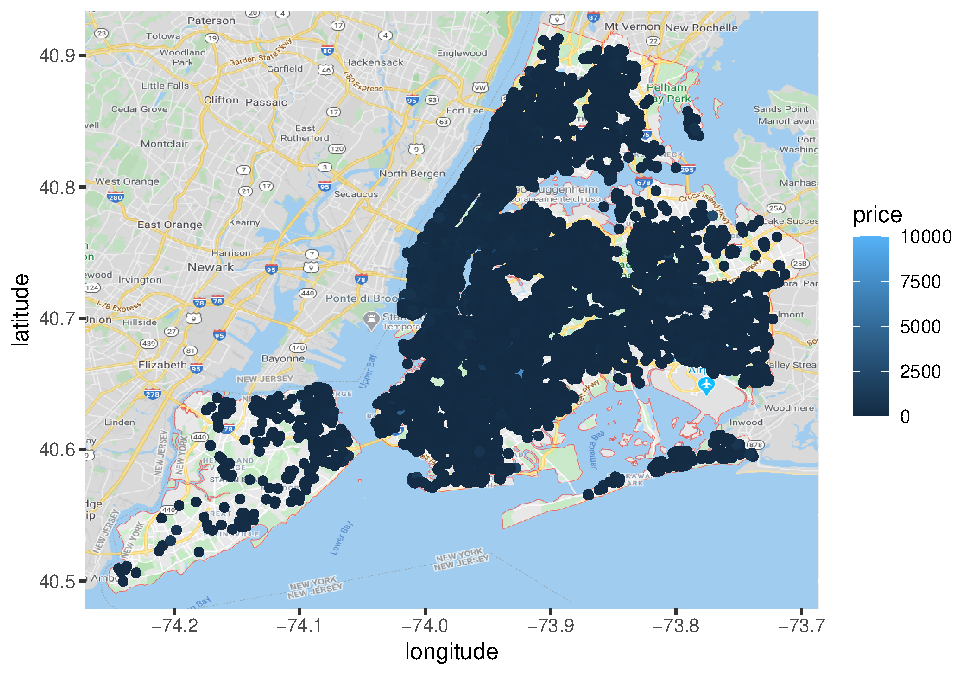
\includegraphics{project_files/figure-latex/unnamed-chunk-3-1.pdf}

\hypertarget{data-cleaning}{%
\section{Data cleaning}\label{data-cleaning}}

\hypertarget{check-for-na-and-null-values}{%
\subsection{Check for NA and NULL
values}\label{check-for-na-and-null-values}}

\begin{Shaded}
\begin{Highlighting}[]
\CommentTok{#Check for NA}
\KeywordTok{apply}\NormalTok{(ds,}\DecValTok{2}\NormalTok{,}\ControlFlowTok{function}\NormalTok{(x) }\KeywordTok{sum}\NormalTok{(}\KeywordTok{is.na}\NormalTok{(x)))}
\end{Highlighting}
\end{Shaded}

\begin{verbatim}
##                             id                           name 
##                              0                              0 
##                        host_id                      host_name 
##                              0                              0 
##            neighbourhood_group                  neighbourhood 
##                              0                              0 
##                       latitude                      longitude 
##                              0                              0 
##                      room_type                          price 
##                              0                              0 
##                 minimum_nights              number_of_reviews 
##                              0                              0 
##                    last_review              reviews_per_month 
##                              0                          10052 
## calculated_host_listings_count               availability_365 
##                              0                              0
\end{verbatim}

\hypertarget{normalisation-and-selection-of-the-variables}{%
\subsection{Normalisation and selection of the
variables}\label{normalisation-and-selection-of-the-variables}}

\begin{Shaded}
\begin{Highlighting}[]
\KeywordTok{library}\NormalTok{(dplyr)}
\KeywordTok{library}\NormalTok{(tidyverse)}
\end{Highlighting}
\end{Shaded}

\begin{verbatim}
## -- Attaching packages ------------------------------------------------------------------------- tidyverse 1.3.0 --
\end{verbatim}

\begin{verbatim}
## v tibble  3.0.1     v stringr 1.4.0
## v readr   1.3.1     v forcats 0.5.0
## v purrr   0.3.4
\end{verbatim}

\begin{verbatim}
## -- Conflicts ---------------------------------------------------------------------------- tidyverse_conflicts() --
## x dplyr::filter() masks stats::filter()
## x dplyr::lag()    masks stats::lag()
\end{verbatim}

\begin{Shaded}
\begin{Highlighting}[]
\NormalTok{normalize <-}\StringTok{ }\ControlFlowTok{function}\NormalTok{(x) \{}
  \KeywordTok{return}\NormalTok{ ((x }\OperatorTok{-}\StringTok{ }\KeywordTok{min}\NormalTok{(x)) }\OperatorTok{/}\StringTok{ }\NormalTok{(}\KeywordTok{max}\NormalTok{(x) }\OperatorTok{-}\StringTok{ }\KeywordTok{min}\NormalTok{(x)))}
\NormalTok{\}}


\NormalTok{clean_data =}\StringTok{ }\ControlFlowTok{function}\NormalTok{(ds, }\DataTypeTok{pr=}\OtherTok{NULL}\NormalTok{, }\DataTypeTok{region=} \OtherTok{NULL}\NormalTok{, }\DataTypeTok{room =} \OtherTok{NULL}\NormalTok{)}
\NormalTok{\{}
\NormalTok{  ds =ds[}\KeywordTok{c}\NormalTok{(}\DecValTok{5}\NormalTok{,}\DecValTok{7}\OperatorTok{:}\DecValTok{10}\NormalTok{)]}
\NormalTok{  ds=}\StringTok{   }\NormalTok{ds}\OperatorTok\KeywordTok{filter}\NormalTok{( price }\OperatorTok{>=}\StringTok{ }\DecValTok{15}\NormalTok{ )}

  \ControlFlowTok{if}\NormalTok{(}\KeywordTok{is.null}\NormalTok{(room))}
\NormalTok{  \{}
\NormalTok{      ds}\OperatorTok{$}\NormalTok{room_type =}\StringTok{ }\KeywordTok{factor}\NormalTok{(ds}\OperatorTok{$}\NormalTok{room_type, }
                        \DataTypeTok{level=} \KeywordTok{c}\NormalTok{(}\StringTok{"Private room"}\NormalTok{,}\StringTok{"Entire home/apt"}\NormalTok{,}\StringTok{"Shared room"}\NormalTok{), }
                        \DataTypeTok{labels=}\KeywordTok{c}\NormalTok{(}\DecValTok{1}\NormalTok{,}\DecValTok{2}\NormalTok{,}\DecValTok{3}\NormalTok{))}
\NormalTok{  \}}
  \ControlFlowTok{else}
\NormalTok{  \{}
\NormalTok{     ds=}\StringTok{   }\NormalTok{ds}\OperatorTok\KeywordTok{filter}\NormalTok{( room_type}\OperatorTok{==}\NormalTok{room)}
\NormalTok{     ds[}\StringTok{"room_type"}\NormalTok{] =}\StringTok{ }\OtherTok{NULL}
\NormalTok{  \}}
   \ControlFlowTok{if}\NormalTok{(}\KeywordTok{is.null}\NormalTok{(region))}
\NormalTok{  \{}

\NormalTok{    ds}\OperatorTok{$}\NormalTok{neighbourhood_group =}\StringTok{ }\KeywordTok{factor}\NormalTok{(ds}\OperatorTok{$}\NormalTok{neighbourhood_group, }
                                  \DataTypeTok{level=} \KeywordTok{c}\NormalTok{(}\StringTok{"Brooklyn"}\NormalTok{,}\StringTok{"Manhattan"}\NormalTok{,}
                                           \StringTok{"Queens"}\NormalTok{,}\StringTok{"Staten Island"}\NormalTok{, }\StringTok{"Bronx"}\NormalTok{),}
                                  \DataTypeTok{labels=}\KeywordTok{c}\NormalTok{(}\DecValTok{1}\NormalTok{,}\DecValTok{2}\NormalTok{,}\DecValTok{3}\NormalTok{,}\DecValTok{4}\NormalTok{,}\DecValTok{5}\NormalTok{))}
\NormalTok{   \}}
  \ControlFlowTok{else}
\NormalTok{  \{}
\NormalTok{      ds=}\StringTok{   }\NormalTok{ds}\OperatorTok\KeywordTok{filter}\NormalTok{( price }\OperatorTok{<}\StringTok{ }\NormalTok{pr }\OperatorTok{&}\StringTok{ }\NormalTok{neighbourhood_group }\OperatorTok{==}\StringTok{ }\NormalTok{region)}
\NormalTok{      ds}\OperatorTok{$}\NormalTok{neighbourhood_group =}\StringTok{ }\OtherTok{NULL}

\NormalTok{  \}}
  \ControlFlowTok{if}\NormalTok{(}\OperatorTok{!}\KeywordTok{is.null}\NormalTok{(pr))}
\NormalTok{  \{}
\NormalTok{    ds=}\StringTok{   }\NormalTok{ds}\OperatorTok\KeywordTok{filter}\NormalTok{( price }\OperatorTok{<}\StringTok{ }\NormalTok{pr )}

\NormalTok{  \}}
\NormalTok{  numerical =}\StringTok{ }\KeywordTok{c}\NormalTok{(}\StringTok{"price"}\NormalTok{)}
\NormalTok{  ds[numerical] =}\StringTok{ }\KeywordTok{as.numeric}\NormalTok{(}\KeywordTok{scale}\NormalTok{(ds[numerical]))}

 
  \KeywordTok{return}\NormalTok{(ds)}
\NormalTok{\}}
\CommentTok{#ggdraw() +}
\CommentTok{#  draw_image("New_York_City_.png") +}
\CommentTok{#  draw_plot(myplot)}

\NormalTok{dataset =}\StringTok{ }\KeywordTok{clean_data}\NormalTok{(ds,}\DecValTok{500}\NormalTok{,}\OtherTok{NULL}\NormalTok{,}\OtherTok{NULL}\NormalTok{)}

\KeywordTok{head}\NormalTok{(dataset)}
\end{Highlighting}
\end{Shaded}

\begin{verbatim}
##   neighbourhood_group latitude longitude room_type      price
## 1                   1 40.64749 -73.97237         1  0.2216662
## 2                   2 40.75362 -73.98377         2  1.1152290
## 3                   2 40.80902 -73.94190         1  0.2334236
## 4                   1 40.68514 -73.95976         2 -0.4837781
## 5                   2 40.79851 -73.94399         2 -0.5895947
## 6                   2 40.74767 -73.97500         2  0.8212939
\end{verbatim}

\begin{Shaded}
\begin{Highlighting}[]
\KeywordTok{summary}\NormalTok{(dataset)}
\end{Highlighting}
\end{Shaded}

\begin{verbatim}
##  neighbourhood_group    latitude       longitude      room_type
##  1:19808             Min.   :40.50   Min.   :-74.24   1:22136  
##  2:20745             1st Qu.:40.69   1st Qu.:-73.98   2:24346  
##  3: 5625             Median :40.72   Median :-73.96   3: 1142  
##  4:  366             Mean   :40.73   Mean   :-73.95            
##  5: 1080             3rd Qu.:40.76   3rd Qu.:-73.94            
##                      Max.   :40.91   Max.   :-73.71            
##      price        
##  Min.   :-1.3538  
##  1st Qu.:-0.7307  
##  Median :-0.3544  
##  Mean   : 0.0000  
##  3rd Qu.: 0.4686  
##  Max.   : 4.3368
\end{verbatim}

\begin{Shaded}
\begin{Highlighting}[]
\NormalTok{mappa =}\StringTok{ }\KeywordTok{ggplot}\NormalTok{()}\OperatorTok{+}\StringTok{ }\KeywordTok{geom_point}\NormalTok{(}\DataTypeTok{data =}\NormalTok{ dataset,  }\KeywordTok{aes}\NormalTok{(}\DataTypeTok{y=}\NormalTok{latitude,}\DataTypeTok{x =}\NormalTok{ longitude, }\DataTypeTok{color =}\NormalTok{ price)) }

 
\NormalTok{mappa}
\end{Highlighting}
\end{Shaded}

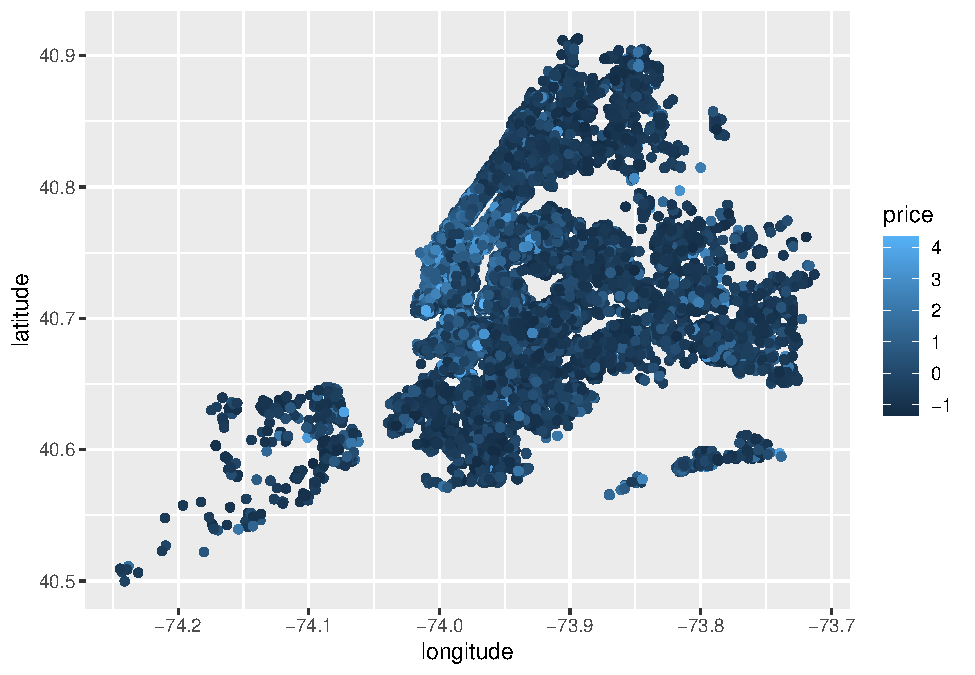
\includegraphics{project_files/figure-latex/unnamed-chunk-6-1.pdf}

\hypertarget{split-data-into-train-and-test-sets}{%
\section{Split data into train and test
sets}\label{split-data-into-train-and-test-sets}}

\begin{Shaded}
\begin{Highlighting}[]
\KeywordTok{library}\NormalTok{(caTools)}
\KeywordTok{library}\NormalTok{(caret)}
\end{Highlighting}
\end{Shaded}

\begin{verbatim}
## Loading required package: lattice
\end{verbatim}

\begin{verbatim}
## 
## Attaching package: 'caret'
\end{verbatim}

\begin{verbatim}
## The following object is masked from 'package:purrr':
## 
##     lift
\end{verbatim}

\begin{Shaded}
\begin{Highlighting}[]
\NormalTok{data_clean =}\StringTok{ }\NormalTok{dataset}
\NormalTok{sample =}\StringTok{ }\KeywordTok{sample.split}\NormalTok{(data_clean, }\DataTypeTok{SplitRatio =} \FloatTok{.75}\NormalTok{)}
\NormalTok{train =}\StringTok{ }\KeywordTok{subset}\NormalTok{(data_clean, sample }\OperatorTok{==}\StringTok{ }\OtherTok{TRUE}\NormalTok{)}
\NormalTok{test  =}\StringTok{ }\KeywordTok{subset}\NormalTok{(data_clean, sample }\OperatorTok{==}\StringTok{ }\OtherTok{FALSE}\NormalTok{)}

\KeywordTok{print}\NormalTok{(}\StringTok{"Initial data shape"}\NormalTok{)}
\end{Highlighting}
\end{Shaded}

\begin{verbatim}
## [1] "Initial data shape"
\end{verbatim}

\begin{Shaded}
\begin{Highlighting}[]
\KeywordTok{print}\NormalTok{(}\KeywordTok{dim}\NormalTok{(data_clean))}
\end{Highlighting}
\end{Shaded}

\begin{verbatim}
## [1] 47624     5
\end{verbatim}

\begin{Shaded}
\begin{Highlighting}[]
\KeywordTok{print}\NormalTok{(}\StringTok{"Train shape"}\NormalTok{)}
\end{Highlighting}
\end{Shaded}

\begin{verbatim}
## [1] "Train shape"
\end{verbatim}

\begin{Shaded}
\begin{Highlighting}[]
\KeywordTok{print}\NormalTok{(}\KeywordTok{dim}\NormalTok{(train))}
\end{Highlighting}
\end{Shaded}

\begin{verbatim}
## [1] 28574     5
\end{verbatim}

\begin{Shaded}
\begin{Highlighting}[]
\KeywordTok{head}\NormalTok{(train)}
\end{Highlighting}
\end{Shaded}

\begin{verbatim}
##    neighbourhood_group latitude longitude room_type      price
## 1                    1 40.64749 -73.97237         1  0.2216662
## 4                    1 40.68514 -73.95976         2 -0.4837781
## 5                    2 40.79851 -73.94399         2 -0.5895947
## 6                    2 40.74767 -73.97500         2  0.8212939
## 9                    2 40.80178 -73.96723         1 -0.6013521
## 10                   2 40.71344 -73.99037         2  0.2334236
\end{verbatim}

\begin{Shaded}
\begin{Highlighting}[]
\KeywordTok{print}\NormalTok{(}\StringTok{"Test shape"}\NormalTok{)}
\end{Highlighting}
\end{Shaded}

\begin{verbatim}
## [1] "Test shape"
\end{verbatim}

\begin{Shaded}
\begin{Highlighting}[]
\KeywordTok{print}\NormalTok{(}\KeywordTok{dim}\NormalTok{(test))}
\end{Highlighting}
\end{Shaded}

\begin{verbatim}
## [1] 19050     5
\end{verbatim}

\begin{Shaded}
\begin{Highlighting}[]
\KeywordTok{head}\NormalTok{(test)}
\end{Highlighting}
\end{Shaded}

\begin{verbatim}
##    neighbourhood_group latitude longitude room_type      price
## 2                    2 40.75362 -73.98377         2  1.1152290
## 3                    2 40.80902 -73.94190         1  0.2334236
## 7                    1 40.68688 -73.95596         1 -0.8247428
## 8                    2 40.76489 -73.98493         1 -0.6013521
## 12                   2 40.76076 -73.98867         1 -0.5308077
## 13                   1 40.66829 -73.98779         1 -0.4837781
\end{verbatim}

\begin{Shaded}
\begin{Highlighting}[]
\KeywordTok{library}\NormalTok{(dplyr)}
\NormalTok{ds_neig =}\StringTok{  }\NormalTok{dataset }\OperatorTok\StringTok{ }\KeywordTok{filter}\NormalTok{(neighbourhood_group }\OperatorTok{==}\StringTok{ }\DecValTok{2}\NormalTok{)}
\NormalTok{ds_neig =}\StringTok{ }\NormalTok{ds_neig[}\OperatorTok{-}\DecValTok{1}\NormalTok{]}


\NormalTok{sample_neig =}\StringTok{ }\KeywordTok{sample.split}\NormalTok{(ds_neig, }\DataTypeTok{SplitRatio =} \FloatTok{.75}\NormalTok{)}
\NormalTok{train_neig =}\StringTok{ }\KeywordTok{subset}\NormalTok{(ds_neig, sample }\OperatorTok{==}\StringTok{ }\OtherTok{TRUE}\NormalTok{)}
\NormalTok{test_neig  =}\StringTok{ }\KeywordTok{subset}\NormalTok{(ds_neig, sample }\OperatorTok{==}\StringTok{ }\OtherTok{FALSE}\NormalTok{)}


\NormalTok{ds_neig_room =}\StringTok{ }\NormalTok{dataset }\OperatorTok\StringTok{ }\KeywordTok{filter}\NormalTok{(neighbourhood_group }\OperatorTok{==}\StringTok{ }\DecValTok{2} \OperatorTok{&}\StringTok{ }\NormalTok{room_type }\OperatorTok{==}\StringTok{ }\DecValTok{1}\NormalTok{)}
\NormalTok{ds_neig_room =}\StringTok{ }\NormalTok{ds_neig_room[}\OperatorTok{-}\DecValTok{1}\NormalTok{][}\OperatorTok{-}\DecValTok{3}\NormalTok{]}

\NormalTok{sample_neig =}\StringTok{ }\KeywordTok{sample.split}\NormalTok{(ds_neig, }\DataTypeTok{SplitRatio =} \FloatTok{.75}\NormalTok{)}
\NormalTok{train_neig_room =}\StringTok{ }\KeywordTok{subset}\NormalTok{(ds_neig_room, sample }\OperatorTok{==}\StringTok{ }\OtherTok{TRUE}\NormalTok{)}
\NormalTok{test_neig_room  =}\StringTok{ }\KeywordTok{subset}\NormalTok{(ds_neig_room, sample }\OperatorTok{==}\StringTok{ }\OtherTok{FALSE}\NormalTok{)}



\KeywordTok{head}\NormalTok{(train_neig)}
\end{Highlighting}
\end{Shaded}

\begin{verbatim}
##    latitude longitude room_type      price
## 1  40.75362 -73.98377         2  1.1152290
## 4  40.74767 -73.97500         2  0.8212939
## 5  40.76489 -73.98493         1 -0.6013521
## 6  40.80178 -73.96723         1 -0.6013521
## 9  40.76076 -73.98867         1 -0.5308077
## 10 40.79826 -73.96113         1 -0.5308077
\end{verbatim}

\begin{Shaded}
\begin{Highlighting}[]
\KeywordTok{head}\NormalTok{(train_neig_room)}
\end{Highlighting}
\end{Shaded}

\begin{verbatim}
##    latitude longitude      price
## 1  40.80902 -73.94190  0.2334236
## 4  40.76076 -73.98867 -0.5308077
## 5  40.79826 -73.96113 -0.5308077
## 6  40.74192 -73.99501  0.1158496
## 9  40.82245 -73.95104 -0.9423169
## 10 40.81305 -73.95466 -0.9188021
\end{verbatim}

\hypertarget{linear-regression}{%
\section{LINEAR REGRESSION}\label{linear-regression}}

\url{https://datascienceplus.com/fitting-neural-network-in-r/}

\begin{Shaded}
\begin{Highlighting}[]
\KeywordTok{cat}\NormalTok{(}\StringTok{"=== Linear Regression without filters ===}\CharTok{\textbackslash{}n}\StringTok{"}\NormalTok{)}
\end{Highlighting}
\end{Shaded}

\begin{verbatim}
## === Linear Regression without filters ===
\end{verbatim}

\begin{Shaded}
\begin{Highlighting}[]
\NormalTok{lm.fit <-}\StringTok{ }\KeywordTok{lm}\NormalTok{(price}\OperatorTok{~}\NormalTok{., }\DataTypeTok{data=}\NormalTok{train)}
\KeywordTok{summary}\NormalTok{(lm.fit)}
\end{Highlighting}
\end{Shaded}

\begin{verbatim}
## 
## Call:
## lm(formula = price ~ ., data = train)
## 
## Residuals:
##     Min      1Q  Median      3Q     Max 
## -2.2793 -0.4490 -0.1397  0.2352  4.8311 
## 
## Coefficients:
##                        Estimate Std. Error t value Pr(>|t|)    
## (Intercept)          -1.949e+02  1.411e+01 -13.807  < 2e-16 ***
## neighbourhood_group2  5.075e-01  1.610e-02  31.528  < 2e-16 ***
## neighbourhood_group3  2.282e-01  1.959e-02  11.646  < 2e-16 ***
## neighbourhood_group4 -9.253e-01  5.836e-02 -15.854  < 2e-16 ***
## neighbourhood_group5  2.685e-01  3.858e-02   6.959 3.49e-12 ***
## latitude             -1.650e+00  1.376e-01 -11.990  < 2e-16 ***
## longitude            -3.533e+00  1.584e-01 -22.304  < 2e-16 ***
## room_type2            1.006e+00  9.549e-03 105.356  < 2e-16 ***
## room_type3           -2.639e-01  3.018e-02  -8.746  < 2e-16 ***
## ---
## Signif. codes:  0 '***' 0.001 '**' 0.01 '*' 0.05 '.' 0.1 ' ' 1
## 
## Residual standard error: 0.7752 on 28565 degrees of freedom
## Multiple R-squared:  0.4014, Adjusted R-squared:  0.4012 
## F-statistic:  2394 on 8 and 28565 DF,  p-value: < 2.2e-16
\end{verbatim}

\begin{Shaded}
\begin{Highlighting}[]
\NormalTok{pr.lm <-}\StringTok{ }\KeywordTok{predict}\NormalTok{(lm.fit,test)}
\NormalTok{MSE.lm <-}\StringTok{ }\KeywordTok{sum}\NormalTok{((pr.lm }\OperatorTok{-}\StringTok{ }\NormalTok{test}\OperatorTok{$}\NormalTok{price)}\OperatorTok{^}\DecValTok{2}\NormalTok{)}\OperatorTok{/}\KeywordTok{nrow}\NormalTok{(test)}
\KeywordTok{cat}\NormalTok{(}\StringTok{"MSE: "}\NormalTok{,MSE.lm)}
\end{Highlighting}
\end{Shaded}

\begin{verbatim}
## MSE:  0.5882613
\end{verbatim}

\begin{Shaded}
\begin{Highlighting}[]
\KeywordTok{plot}\NormalTok{(lm.fit)}
\end{Highlighting}
\end{Shaded}

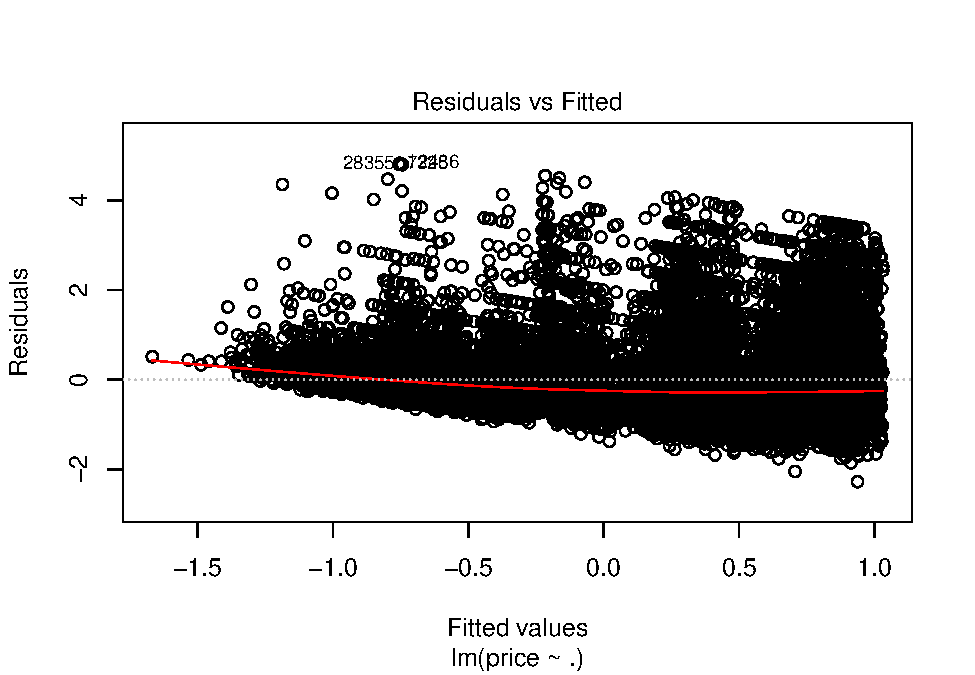
\includegraphics{project_files/figure-latex/unnamed-chunk-9-1.pdf}
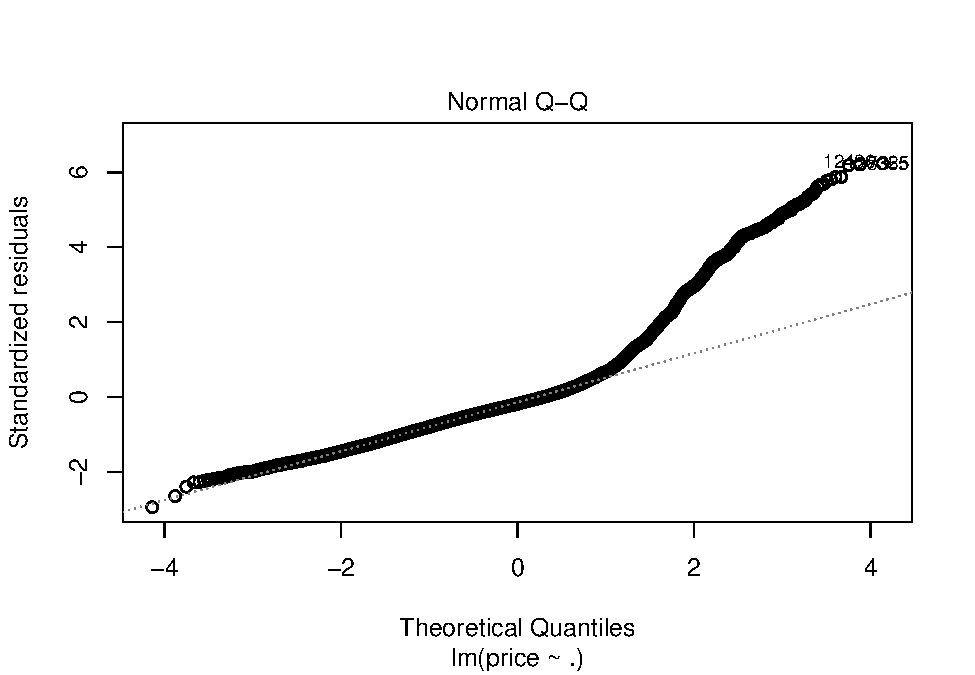
\includegraphics{project_files/figure-latex/unnamed-chunk-9-2.pdf}
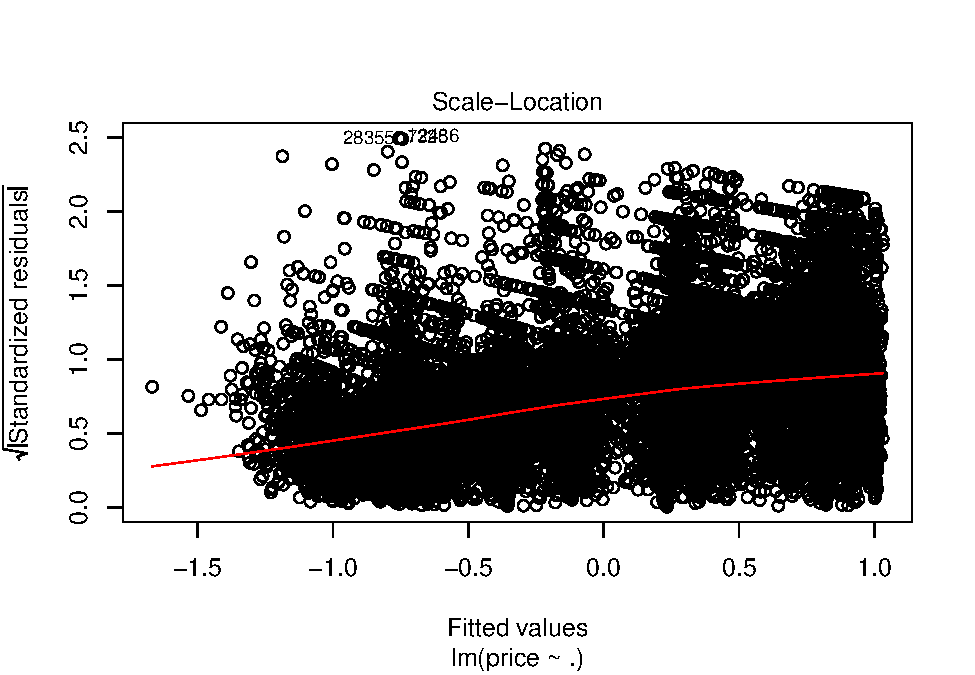
\includegraphics{project_files/figure-latex/unnamed-chunk-9-3.pdf}
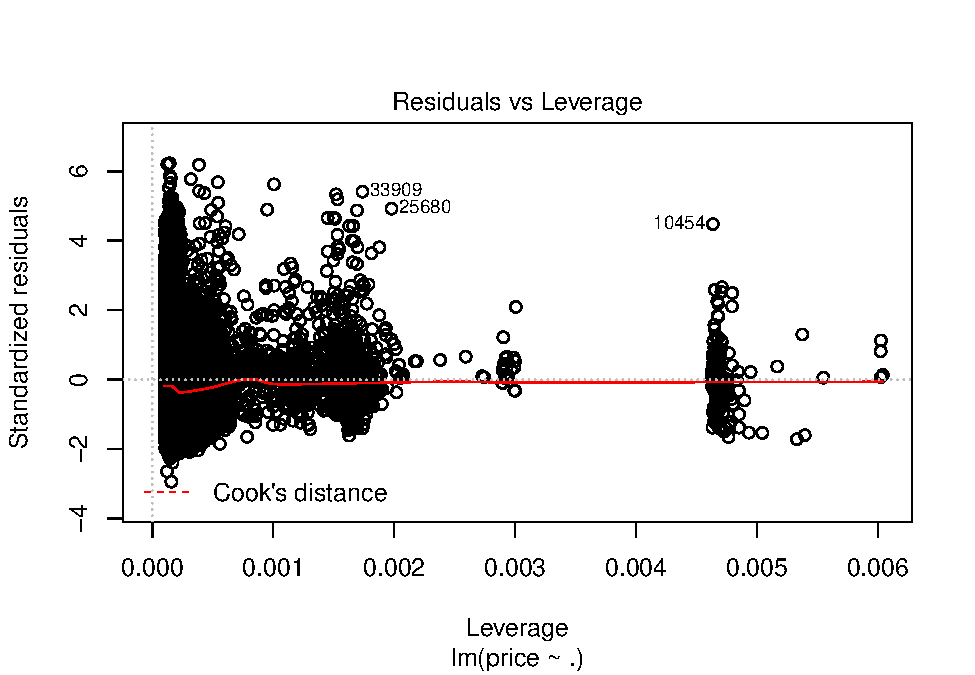
\includegraphics{project_files/figure-latex/unnamed-chunk-9-4.pdf}

\begin{Shaded}
\begin{Highlighting}[]
\KeywordTok{library}\NormalTok{(dplyr)}

\KeywordTok{cat}\NormalTok{(}\StringTok{" === Linear Regression selecting the Neighboorhood group === }\CharTok{\textbackslash{}n}\StringTok{"}\NormalTok{)}
\end{Highlighting}
\end{Shaded}

\begin{verbatim}
##  === Linear Regression selecting the Neighboorhood group ===
\end{verbatim}

\begin{Shaded}
\begin{Highlighting}[]
\KeywordTok{cat}\NormalTok{(}\StringTok{"Neighboorhood group = Manhattan}\CharTok{\textbackslash{}n}\StringTok{ "}\NormalTok{)}
\end{Highlighting}
\end{Shaded}

\begin{verbatim}
## Neighboorhood group = Manhattan
## 
\end{verbatim}

\begin{Shaded}
\begin{Highlighting}[]
\NormalTok{lm2.fit <-}\StringTok{ }\KeywordTok{lm}\NormalTok{(price}\OperatorTok{~}\NormalTok{., }\DataTypeTok{data=}\NormalTok{train_neig)}
\KeywordTok{summary}\NormalTok{(lm2.fit)}
\end{Highlighting}
\end{Shaded}

\begin{verbatim}
## 
## Call:
## lm(formula = price ~ ., data = train_neig)
## 
## Residuals:
##     Min      1Q  Median      3Q     Max 
## -2.4448 -0.5335 -0.1821  0.2943  4.6021 
## 
## Coefficients:
##               Estimate Std. Error t value Pr(>|t|)    
## (Intercept) -818.70943   65.28262 -12.541  < 2e-16 ***
## latitude      -0.59342    0.39541  -1.501    0.133    
## longitude    -11.39120    0.68958 -16.519  < 2e-16 ***
## room_type2     1.03307    0.01667  61.966  < 2e-16 ***
## room_type3    -0.25086    0.05346  -4.692 2.73e-06 ***
## ---
## Signif. codes:  0 '***' 0.001 '**' 0.01 '*' 0.05 '.' 0.1 ' ' 1
## 
## Residual standard error: 0.8717 on 12442 degrees of freedom
## Multiple R-squared:  0.3434, Adjusted R-squared:  0.3432 
## F-statistic:  1627 on 4 and 12442 DF,  p-value: < 2.2e-16
\end{verbatim}

\begin{Shaded}
\begin{Highlighting}[]
\NormalTok{pr2.lm <-}\StringTok{ }\KeywordTok{predict}\NormalTok{(lm2.fit,test_neig)}
\NormalTok{MSE2.lm <-}\StringTok{ }\KeywordTok{sum}\NormalTok{((pr2.lm }\OperatorTok{-}\StringTok{ }\NormalTok{test_neig}\OperatorTok{$}\NormalTok{price)}\OperatorTok{^}\DecValTok{2}\NormalTok{)}\OperatorTok{/}\KeywordTok{nrow}\NormalTok{(test_neig)}

\KeywordTok{cat}\NormalTok{(}\StringTok{"MSE: "}\NormalTok{,MSE2.lm)}
\end{Highlighting}
\end{Shaded}

\begin{verbatim}
## MSE:  0.7394892
\end{verbatim}

\begin{Shaded}
\begin{Highlighting}[]
\KeywordTok{plot}\NormalTok{(lm2.fit)}
\end{Highlighting}
\end{Shaded}

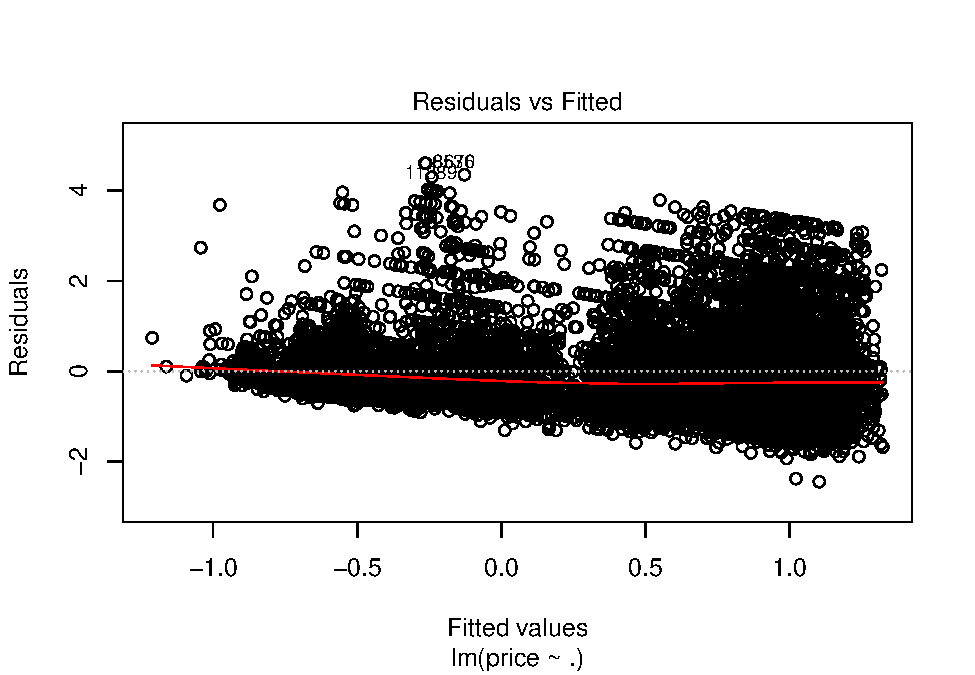
\includegraphics{project_files/figure-latex/unnamed-chunk-10-1.pdf}
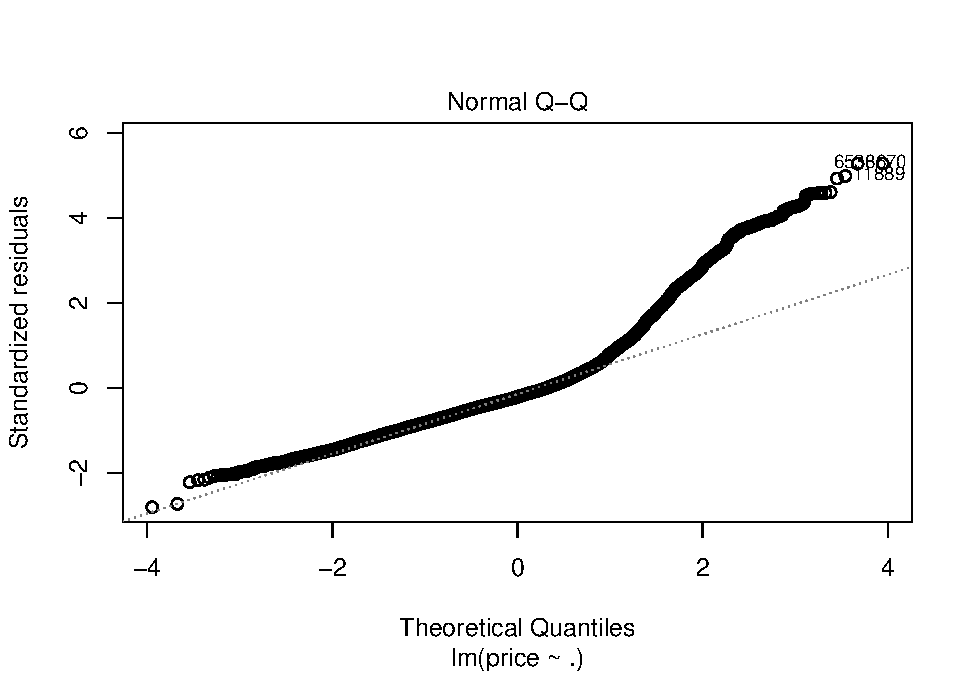
\includegraphics{project_files/figure-latex/unnamed-chunk-10-2.pdf}
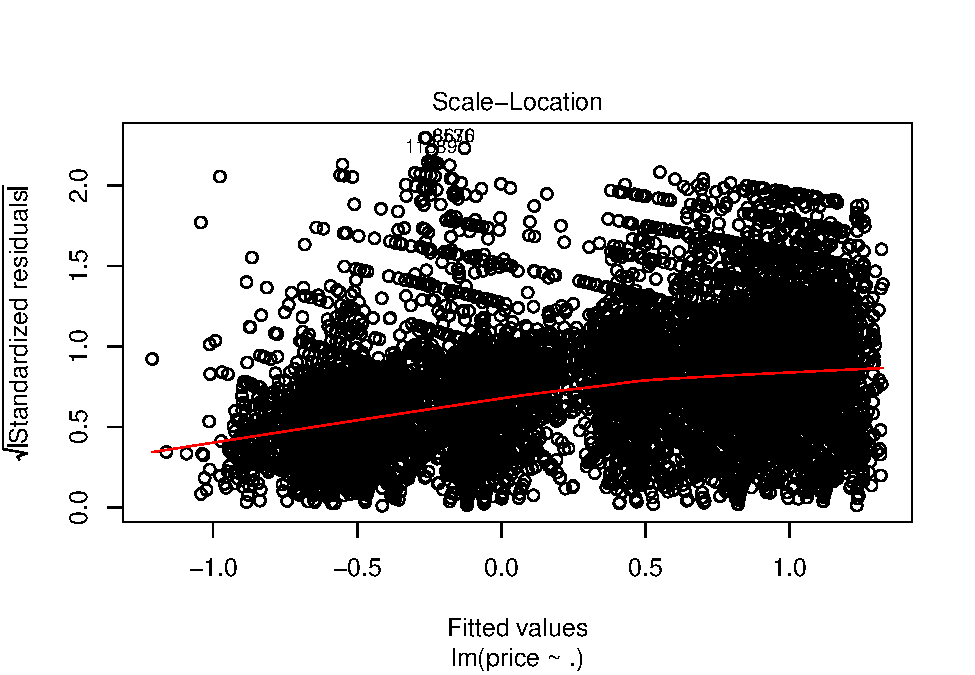
\includegraphics{project_files/figure-latex/unnamed-chunk-10-3.pdf}
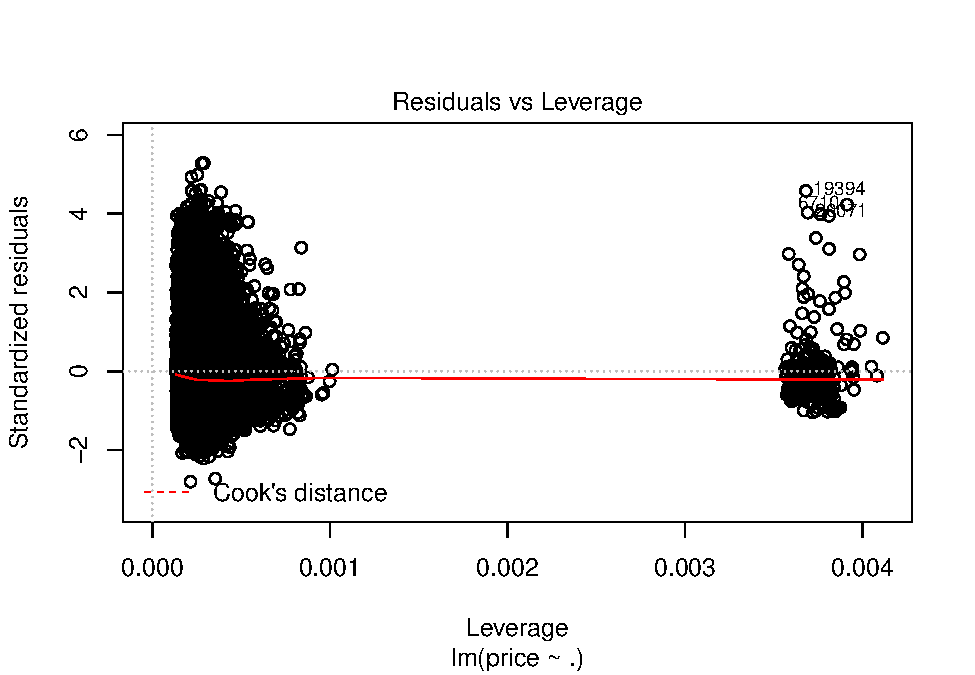
\includegraphics{project_files/figure-latex/unnamed-chunk-10-4.pdf}

\begin{Shaded}
\begin{Highlighting}[]
\KeywordTok{library}\NormalTok{(dplyr)}

\KeywordTok{cat}\NormalTok{(}\StringTok{"=== Linear Regression selecting the Neighboorhood group and room_type ===}\CharTok{\textbackslash{}n}\StringTok{"}\NormalTok{)}
\end{Highlighting}
\end{Shaded}

\begin{verbatim}
## === Linear Regression selecting the Neighboorhood group and room_type ===
\end{verbatim}

\begin{Shaded}
\begin{Highlighting}[]
\KeywordTok{cat}\NormalTok{(}\StringTok{"Neighboorhood group = Manhattan and room_type = Entire home/apt}\CharTok{\textbackslash{}n}\StringTok{ "}\NormalTok{)}
\end{Highlighting}
\end{Shaded}

\begin{verbatim}
## Neighboorhood group = Manhattan and room_type = Entire home/apt
## 
\end{verbatim}

\begin{Shaded}
\begin{Highlighting}[]
\NormalTok{lm3.fit <-}\StringTok{ }\KeywordTok{lm}\NormalTok{(price}\OperatorTok{~}\NormalTok{., }\DataTypeTok{data=}\NormalTok{train_neig_room)}
\KeywordTok{summary}\NormalTok{(lm3.fit)}
\end{Highlighting}
\end{Shaded}

\begin{verbatim}
## 
## Call:
## lm(formula = price ~ ., data = train_neig_room)
## 
## Residuals:
##     Min      1Q  Median      3Q     Max 
## -1.2556 -0.3793 -0.1637  0.1439  4.6078 
## 
## Coefficients:
##              Estimate Std. Error t value Pr(>|t|)    
## (Intercept) -649.0529    83.2867  -7.793    8e-15 ***
## latitude      -0.7457     0.4795  -1.555     0.12    
## longitude     -9.1815     0.8867 -10.354   <2e-16 ***
## ---
## Signif. codes:  0 '***' 0.001 '**' 0.01 '*' 0.05 '.' 0.1 ' ' 1
## 
## Residual standard error: 0.666 on 4714 degrees of freedom
## Multiple R-squared:  0.1134, Adjusted R-squared:  0.113 
## F-statistic: 301.4 on 2 and 4714 DF,  p-value: < 2.2e-16
\end{verbatim}

\begin{Shaded}
\begin{Highlighting}[]
\NormalTok{pr3.lm <-}\StringTok{ }\KeywordTok{predict}\NormalTok{(lm3.fit,test_neig_room)}
\NormalTok{MSE3.lm <-}\StringTok{ }\KeywordTok{sum}\NormalTok{((pr3.lm }\OperatorTok{-}\StringTok{ }\NormalTok{test_neig_room}\OperatorTok{$}\NormalTok{price)}\OperatorTok{^}\DecValTok{2}\NormalTok{)}\OperatorTok{/}\KeywordTok{nrow}\NormalTok{(test_neig_room)}

\KeywordTok{cat}\NormalTok{(}\StringTok{"MSE: "}\NormalTok{,MSE3.lm)}
\end{Highlighting}
\end{Shaded}

\begin{verbatim}
## MSE:  0.4265148
\end{verbatim}

\begin{Shaded}
\begin{Highlighting}[]
\KeywordTok{plot}\NormalTok{(lm3.fit)}
\end{Highlighting}
\end{Shaded}

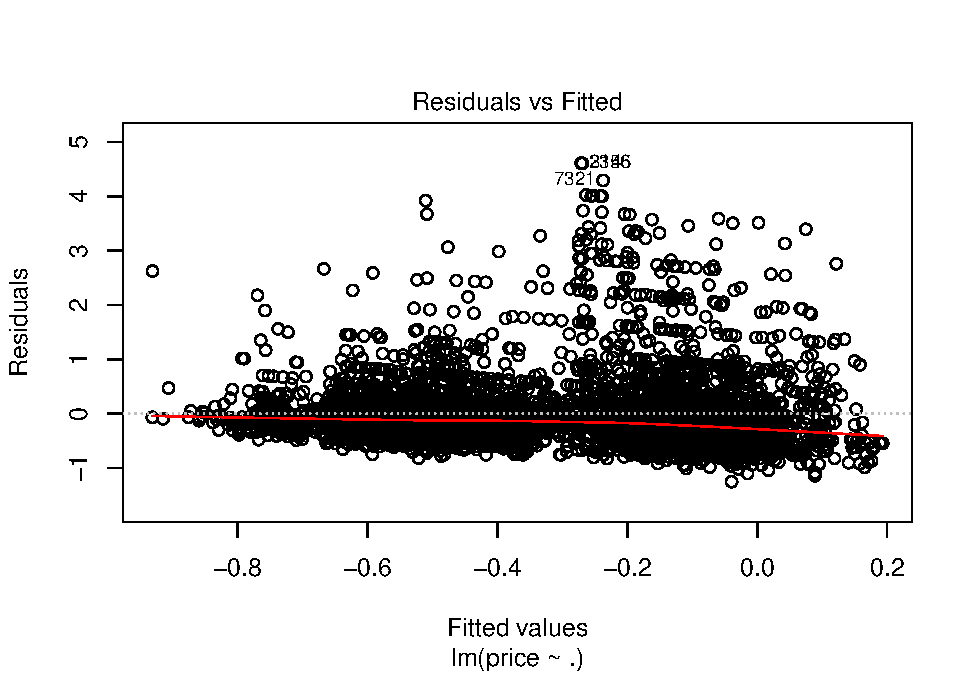
\includegraphics{project_files/figure-latex/unnamed-chunk-11-1.pdf}
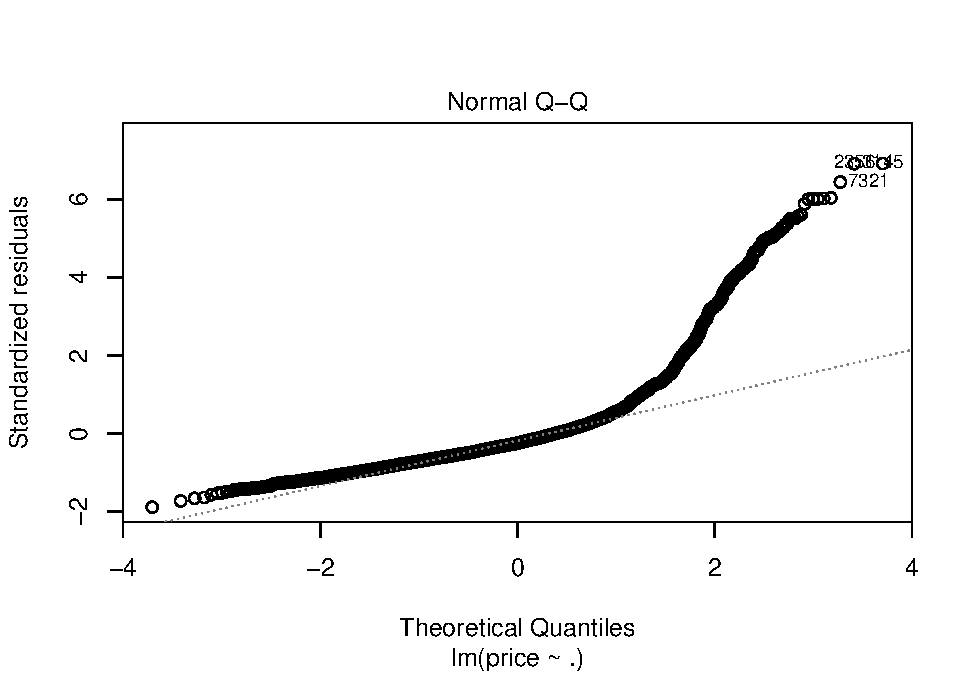
\includegraphics{project_files/figure-latex/unnamed-chunk-11-2.pdf}
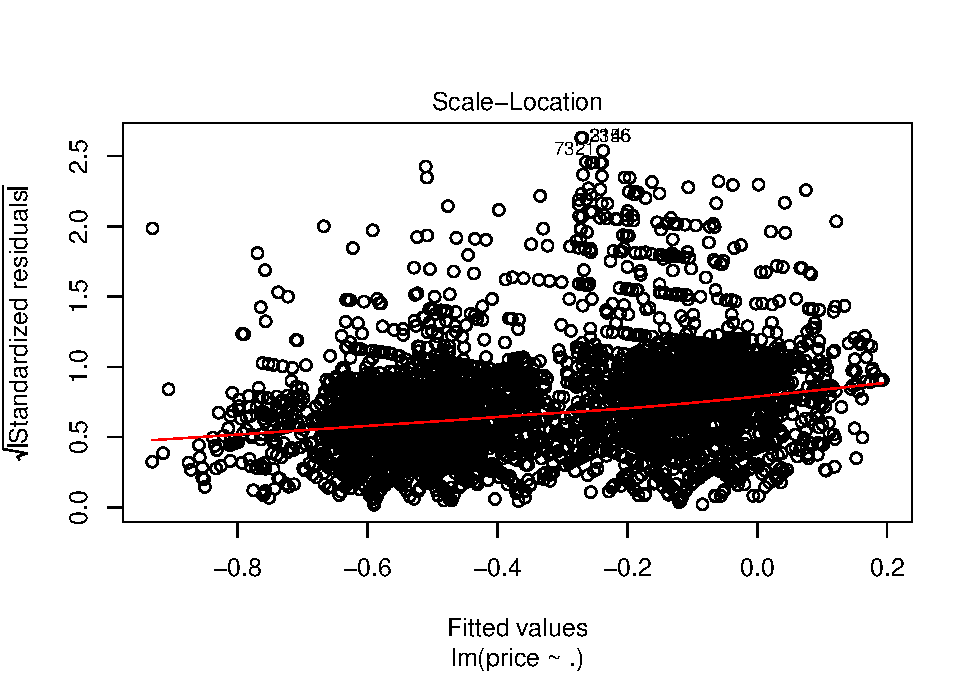
\includegraphics{project_files/figure-latex/unnamed-chunk-11-3.pdf}
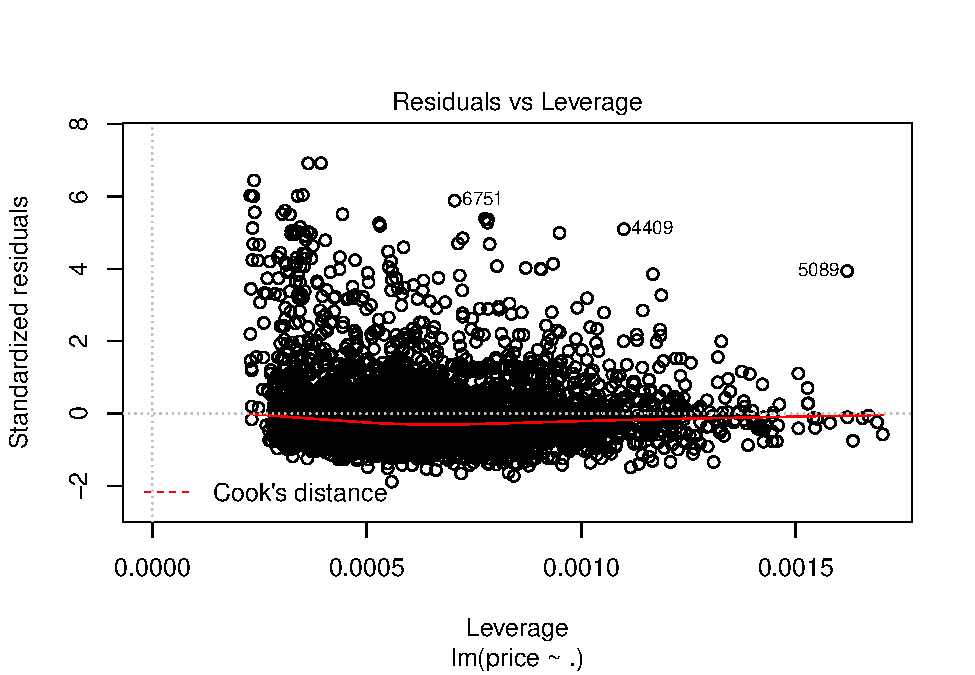
\includegraphics{project_files/figure-latex/unnamed-chunk-11-4.pdf}

\begin{Shaded}
\begin{Highlighting}[]
\KeywordTok{par}\NormalTok{(}\DataTypeTok{mfrow=}\KeywordTok{c}\NormalTok{(}\DecValTok{1}\NormalTok{,}\DecValTok{2}\NormalTok{))}
\CommentTok{#plot(test$price,nn_pred$net.result,col='red',main='Real vs predicted NN',pch=18,cex=0.7)}
\CommentTok{#abline(0,1,lwd=2)}
\CommentTok{#legend('bottomright',legend='NN',pch=18,col='red', bty='n')}
\KeywordTok{plot}\NormalTok{(test}\OperatorTok{$}\NormalTok{price,pr.lm,}\DataTypeTok{col=}\StringTok{'red'}\NormalTok{,}\DataTypeTok{main=}\StringTok{'Real vs predicted LN'}\NormalTok{,}\DataTypeTok{pch=}\DecValTok{18}\NormalTok{, }\DataTypeTok{cex=}\FloatTok{0.7}\NormalTok{)}
\KeywordTok{abline}\NormalTok{(}\DecValTok{0}\NormalTok{,}\DecValTok{1}\NormalTok{,}\DataTypeTok{lwd=}\DecValTok{2}\NormalTok{)}
\KeywordTok{legend}\NormalTok{(}\StringTok{'bottomright'}\NormalTok{,}\DataTypeTok{legend=}\StringTok{'LM'}\NormalTok{,}\DataTypeTok{pch=}\DecValTok{18}\NormalTok{,}\DataTypeTok{col=}\StringTok{'red'}\NormalTok{, }\DataTypeTok{bty=}\StringTok{'n'}\NormalTok{, }\DataTypeTok{cex=}\NormalTok{.}\DecValTok{95}\NormalTok{)}
\end{Highlighting}
\end{Shaded}

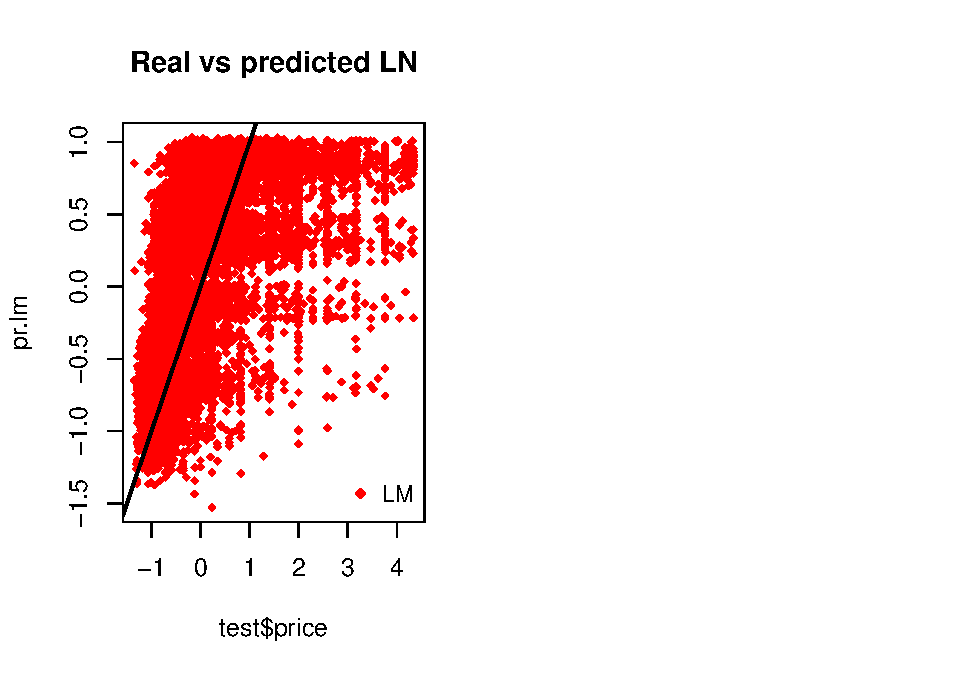
\includegraphics{project_files/figure-latex/unnamed-chunk-12-1.pdf}

\hypertarget{decision-tree}{%
\section{DECISION TREE}\label{decision-tree}}

library(rpart) library(caret) library(e1071)

dt = train( price\textasciitilde{} ., data = train,method = ``rpart'')
pred2 = predict(dt, data = test\(price) table(pred2, test\)price)

\begin{Shaded}
\begin{Highlighting}[]
\KeywordTok{library}\NormalTok{(tree)}
\end{Highlighting}
\end{Shaded}

\begin{verbatim}
## Registered S3 method overwritten by 'tree':
##   method     from
##   print.tree cli
\end{verbatim}

\begin{Shaded}
\begin{Highlighting}[]
\KeywordTok{library}\NormalTok{(MASS)}
\end{Highlighting}
\end{Shaded}

\begin{verbatim}
## 
## Attaching package: 'MASS'
\end{verbatim}

\begin{verbatim}
## The following object is masked from 'package:dplyr':
## 
##     select
\end{verbatim}

\begin{Shaded}
\begin{Highlighting}[]
\NormalTok{tree_reg =}\KeywordTok{tree}\NormalTok{(price}\OperatorTok{~}\NormalTok{., }\DataTypeTok{data =}\NormalTok{ train)}
\KeywordTok{cat}\NormalTok{(}\StringTok{" === Decision Tree without filters === }\CharTok{\textbackslash{}n}\StringTok{"}\NormalTok{)}
\end{Highlighting}
\end{Shaded}

\begin{verbatim}
##  === Decision Tree without filters ===
\end{verbatim}

\begin{Shaded}
\begin{Highlighting}[]
\KeywordTok{summary}\NormalTok{(tree_reg)}
\end{Highlighting}
\end{Shaded}

\begin{verbatim}
## 
## Regression tree:
## tree(formula = price ~ ., data = train)
## Variables actually used in tree construction:
## [1] "room_type" "longitude" "latitude" 
## Number of terminal nodes:  5 
## Residual mean deviance:  0.597 = 17050 / 28570 
## Distribution of residuals:
##    Min. 1st Qu.  Median    Mean 3rd Qu.    Max. 
## -2.3320 -0.4249 -0.1427  0.0000  0.2266  4.7770
\end{verbatim}

\begin{Shaded}
\begin{Highlighting}[]
\NormalTok{yhat=}\KeywordTok{predict}\NormalTok{(tree_reg,test)}
\NormalTok{tree_reg_mse =}\StringTok{ }\KeywordTok{mean}\NormalTok{((yhat}\OperatorTok{-}\NormalTok{test}\OperatorTok{$}\NormalTok{price)}\OperatorTok{^}\DecValTok{2}\NormalTok{)}
\NormalTok{tree_reg_mse}
\end{Highlighting}
\end{Shaded}

\begin{verbatim}
## [1] 0.5825501
\end{verbatim}

\begin{Shaded}
\begin{Highlighting}[]
\KeywordTok{plot}\NormalTok{(tree_reg)}
\KeywordTok{text}\NormalTok{(tree_reg,}\DataTypeTok{pretty=}\DecValTok{0}\NormalTok{)}
\end{Highlighting}
\end{Shaded}

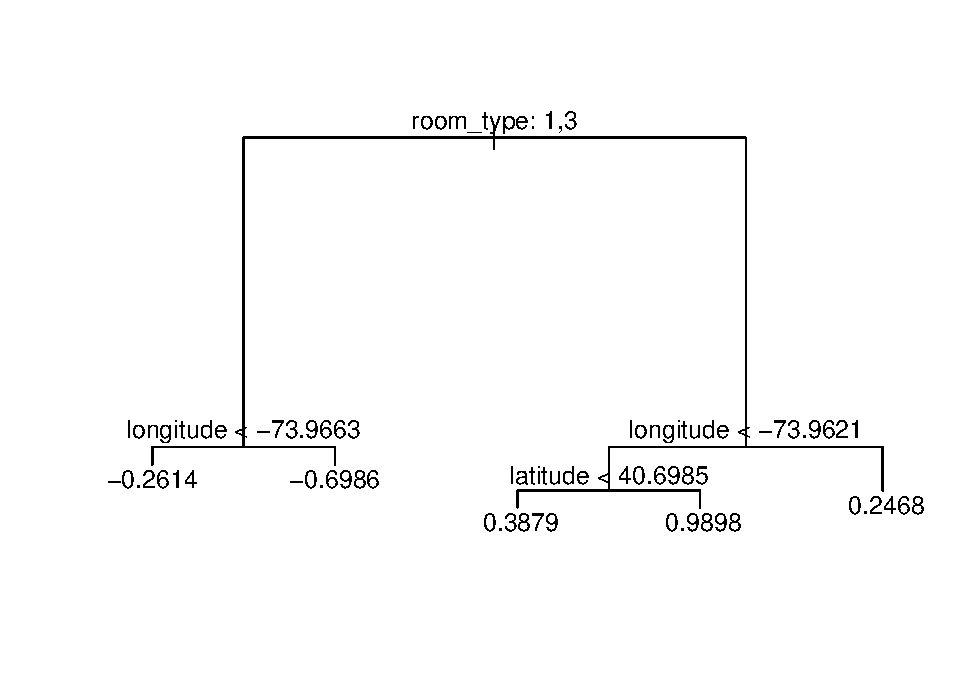
\includegraphics{project_files/figure-latex/unnamed-chunk-13-1.pdf}

\begin{Shaded}
\begin{Highlighting}[]
\KeywordTok{cat}\NormalTok{(}\StringTok{" === Decision Tree selecting the Neighboorhood group === }\CharTok{\textbackslash{}n}\StringTok{"}\NormalTok{)}
\end{Highlighting}
\end{Shaded}

\begin{verbatim}
##  === Decision Tree selecting the Neighboorhood group ===
\end{verbatim}

\begin{Shaded}
\begin{Highlighting}[]
\KeywordTok{cat}\NormalTok{(}\StringTok{"Neighboorhood group = Manhattan}\CharTok{\textbackslash{}n}\StringTok{ "}\NormalTok{)}
\end{Highlighting}
\end{Shaded}

\begin{verbatim}
## Neighboorhood group = Manhattan
## 
\end{verbatim}

\begin{Shaded}
\begin{Highlighting}[]
\NormalTok{tree_reg =}\KeywordTok{tree}\NormalTok{(price}\OperatorTok{~}\NormalTok{., }\DataTypeTok{data =}\NormalTok{ train_neig)}
\KeywordTok{summary}\NormalTok{(tree_reg)}
\end{Highlighting}
\end{Shaded}

\begin{verbatim}
## 
## Regression tree:
## tree(formula = price ~ ., data = train_neig)
## Number of terminal nodes:  4 
## Residual mean deviance:  0.765 = 9519 / 12440 
## Distribution of residuals:
##    Min. 1st Qu.  Median    Mean 3rd Qu.    Max. 
## -2.3370 -0.5146 -0.1737  0.0000  0.3245  4.4420
\end{verbatim}

\begin{Shaded}
\begin{Highlighting}[]
\NormalTok{tree_reg_mse =}\StringTok{ }\KeywordTok{mean}\NormalTok{((}\KeywordTok{predict}\NormalTok{(tree_reg,test_neig)}\OperatorTok{-}\NormalTok{test_neig}\OperatorTok{$}\NormalTok{price)}\OperatorTok{^}\DecValTok{2}\NormalTok{)}
\NormalTok{tree_reg_mse}
\end{Highlighting}
\end{Shaded}

\begin{verbatim}
## [1] 0.7466177
\end{verbatim}

\begin{Shaded}
\begin{Highlighting}[]
\KeywordTok{plot}\NormalTok{(tree_reg)}
\KeywordTok{text}\NormalTok{(tree_reg,}\DataTypeTok{pretty=}\DecValTok{1}\NormalTok{)}
\end{Highlighting}
\end{Shaded}

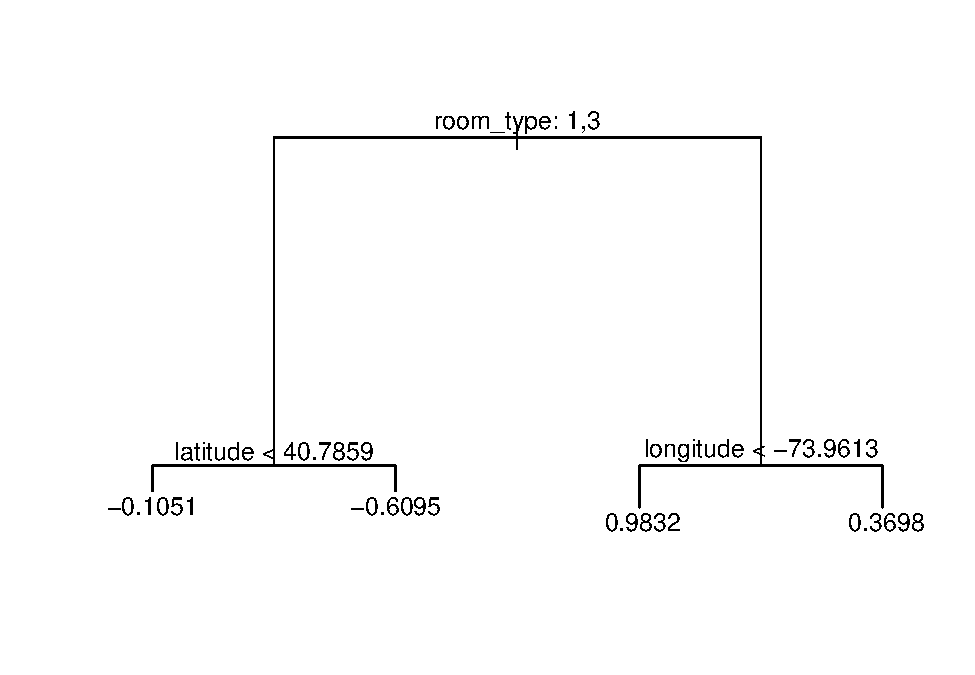
\includegraphics{project_files/figure-latex/unnamed-chunk-14-1.pdf}

\begin{Shaded}
\begin{Highlighting}[]
\KeywordTok{cat}\NormalTok{(}\StringTok{"=== Decision Tree selecting the Neighboorhood group and room_type ===}\CharTok{\textbackslash{}n}\StringTok{"}\NormalTok{)}
\end{Highlighting}
\end{Shaded}

\begin{verbatim}
## === Decision Tree selecting the Neighboorhood group and room_type ===
\end{verbatim}

\begin{Shaded}
\begin{Highlighting}[]
\KeywordTok{cat}\NormalTok{(}\StringTok{"Neighboorhood group = Manhattan and room_type = Entire home/apt}\CharTok{\textbackslash{}n}\StringTok{ "}\NormalTok{)}
\end{Highlighting}
\end{Shaded}

\begin{verbatim}
## Neighboorhood group = Manhattan and room_type = Entire home/apt
## 
\end{verbatim}

\begin{Shaded}
\begin{Highlighting}[]
\NormalTok{tree_reg =}\KeywordTok{tree}\NormalTok{(price}\OperatorTok{~}\NormalTok{., }\DataTypeTok{data =}\NormalTok{ train_neig_room)}
\KeywordTok{summary}\NormalTok{(tree_reg)}
\end{Highlighting}
\end{Shaded}

\begin{verbatim}
## 
## Regression tree:
## tree(formula = price ~ ., data = train_neig_room)
## Number of terminal nodes:  6 
## Residual mean deviance:  0.394 = 1856 / 4711 
## Distribution of residuals:
##    Min. 1st Qu.  Median    Mean 3rd Qu.    Max. 
## -2.3290 -0.3540 -0.1358  0.0000  0.1327  3.9750
\end{verbatim}

\begin{Shaded}
\begin{Highlighting}[]
\NormalTok{tree_reg_mse =}\StringTok{ }\KeywordTok{mean}\NormalTok{((}\KeywordTok{predict}\NormalTok{(tree_reg,test_neig_room)}\OperatorTok{-}\NormalTok{test_neig_room}\OperatorTok{$}\NormalTok{price)}\OperatorTok{^}\DecValTok{2}\NormalTok{)}
\NormalTok{tree_reg_mse}
\end{Highlighting}
\end{Shaded}

\begin{verbatim}
## [1] 0.4019698
\end{verbatim}

\begin{Shaded}
\begin{Highlighting}[]
\KeywordTok{plot}\NormalTok{(tree_reg)}
\KeywordTok{text}\NormalTok{(tree_reg,}\DataTypeTok{pretty=}\DecValTok{0}\NormalTok{)}
\end{Highlighting}
\end{Shaded}

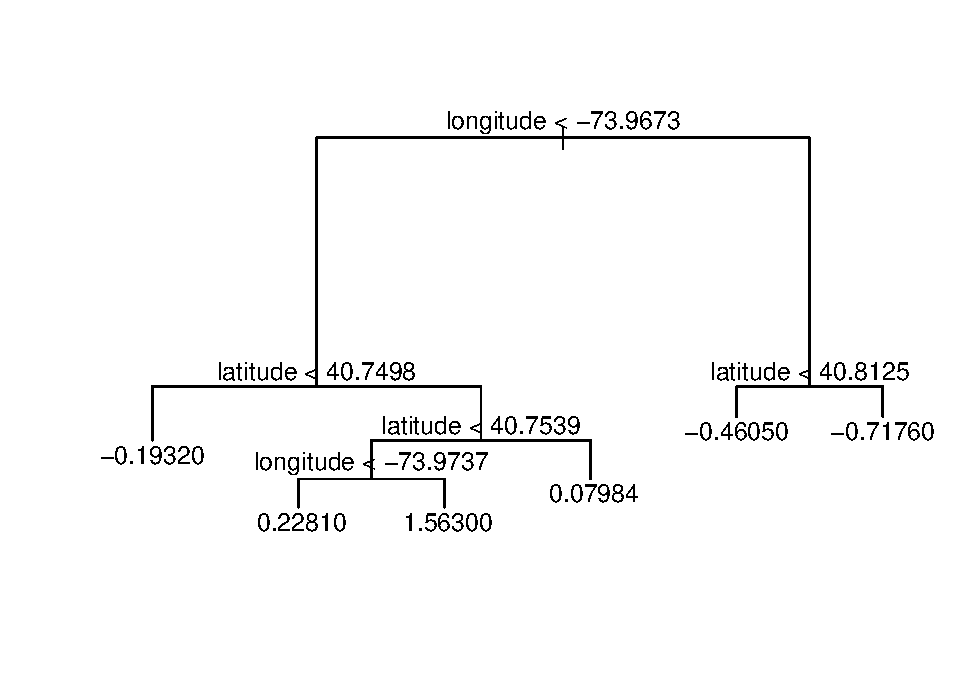
\includegraphics{project_files/figure-latex/unnamed-chunk-15-1.pdf}

\begin{Shaded}
\begin{Highlighting}[]
\NormalTok{test}\OperatorTok{$}\NormalTok{price =}\StringTok{ }\KeywordTok{as.numeric}\NormalTok{(test}\OperatorTok{$}\NormalTok{price)}
\NormalTok{tree_reg.pred=}\KeywordTok{predict}\NormalTok{(tree_reg, test)}
\CommentTok{#table(tree_reg.pred,test$price)}

\KeywordTok{par}\NormalTok{(}\DataTypeTok{mfrow=}\KeywordTok{c}\NormalTok{(}\DecValTok{1}\NormalTok{,}\DecValTok{2}\NormalTok{))}
\KeywordTok{plot}\NormalTok{(}\KeywordTok{as.numeric}\NormalTok{(test}\OperatorTok{$}\NormalTok{price),tree_reg.pred,}\DataTypeTok{col=}\StringTok{'red'}\NormalTok{,}\DataTypeTok{main=}\StringTok{'Real vs predicted Tree Regressor'}\NormalTok{,}\DataTypeTok{pch=}\DecValTok{18}\NormalTok{,}\DataTypeTok{cex=}\FloatTok{0.7}\NormalTok{)}
\KeywordTok{legend}\NormalTok{(}\StringTok{'bottomright'}\NormalTok{,}\DataTypeTok{legend=}\StringTok{'TR'}\NormalTok{,}\DataTypeTok{pch=}\DecValTok{18}\NormalTok{,}\DataTypeTok{col=}\StringTok{'red'}\NormalTok{, }\DataTypeTok{bty=}\StringTok{'n'}\NormalTok{)}
\end{Highlighting}
\end{Shaded}

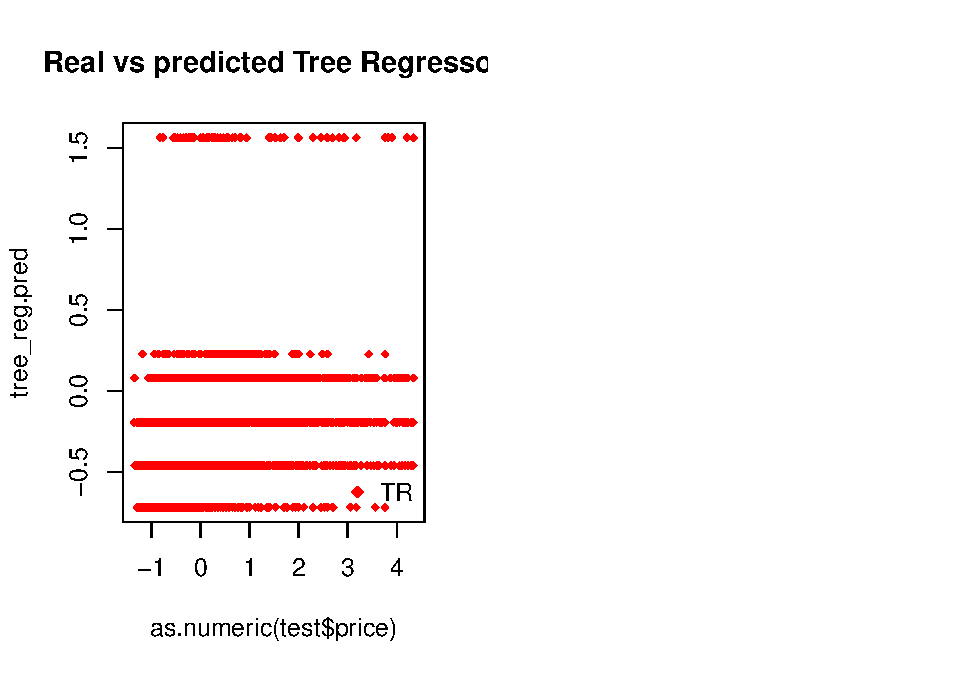
\includegraphics{project_files/figure-latex/unnamed-chunk-16-1.pdf}

\begin{Shaded}
\begin{Highlighting}[]
\NormalTok{yhat=}\KeywordTok{predict}\NormalTok{(tree_reg,test)}
\KeywordTok{plot}\NormalTok{(yhat,test}\OperatorTok{$}\NormalTok{price)}
\KeywordTok{abline}\NormalTok{(}\DecValTok{0}\NormalTok{,}\DecValTok{1}\NormalTok{)}
\end{Highlighting}
\end{Shaded}

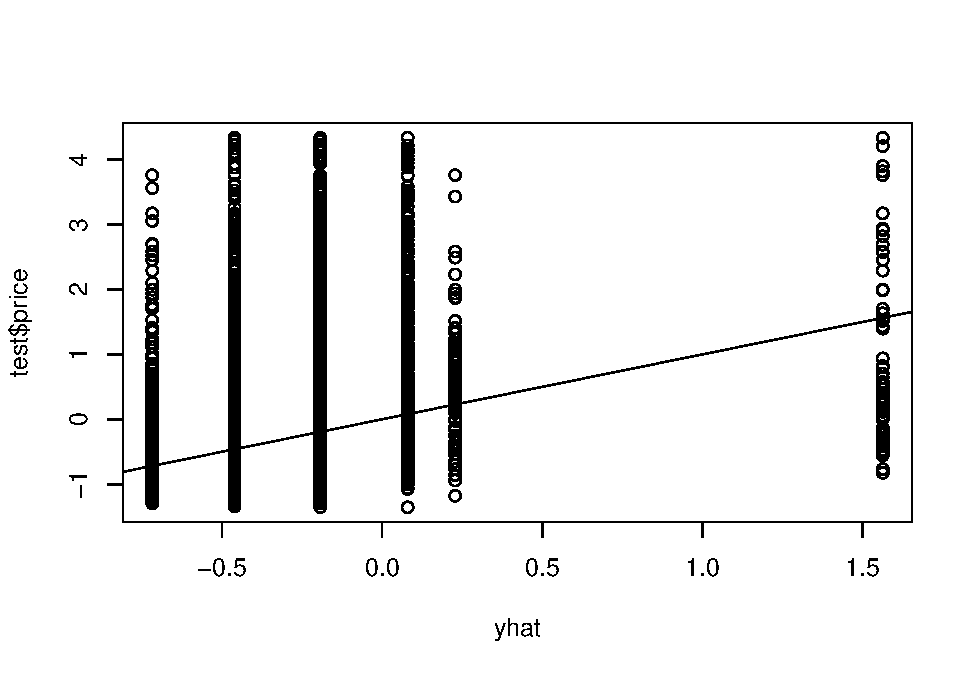
\includegraphics{project_files/figure-latex/unnamed-chunk-17-1.pdf}

\begin{Shaded}
\begin{Highlighting}[]
\NormalTok{tree_reg_mse =}\StringTok{ }\KeywordTok{mean}\NormalTok{((yhat}\OperatorTok{-}\NormalTok{test}\OperatorTok{$}\NormalTok{price)}\OperatorTok{^}\DecValTok{2}\NormalTok{)}
\NormalTok{tree_reg_mse}
\end{Highlighting}
\end{Shaded}

\begin{verbatim}
## [1] 1.010335
\end{verbatim}

\hypertarget{random-forest}{%
\section{RANDOM FOREST}\label{random-forest}}

\url{https://www.guru99.com/r-random-forest-tutorial.html}

GOOD VIDEO FOR PARAMETER OPTIMISATION
\url{https://www.youtube.com/watch?v=6EXPYzbfLCE}

TUNING \url{https://uc-r.github.io/random_forests}

\begin{Shaded}
\begin{Highlighting}[]
\KeywordTok{library}\NormalTok{(randomForest)}
\end{Highlighting}
\end{Shaded}

\begin{verbatim}
## randomForest 4.6-14
\end{verbatim}

\begin{verbatim}
## Type rfNews() to see new features/changes/bug fixes.
\end{verbatim}

\begin{verbatim}
## 
## Attaching package: 'randomForest'
\end{verbatim}

\begin{verbatim}
## The following object is masked from 'package:dplyr':
## 
##     combine
\end{verbatim}

\begin{verbatim}
## The following object is masked from 'package:ggplot2':
## 
##     margin
\end{verbatim}

\begin{Shaded}
\begin{Highlighting}[]
\KeywordTok{cat}\NormalTok{(}\StringTok{" === Random Forest without filters === }\CharTok{\textbackslash{}n}\StringTok{"}\NormalTok{)}
\end{Highlighting}
\end{Shaded}

\begin{verbatim}
##  === Random Forest without filters ===
\end{verbatim}

\begin{Shaded}
\begin{Highlighting}[]
\NormalTok{rf <-}\StringTok{ }\KeywordTok{randomForest}\NormalTok{(}
\NormalTok{  price }\OperatorTok{~}\StringTok{ }\NormalTok{. ,}
  \DataTypeTok{data=}\NormalTok{train,}
\NormalTok{)}
\NormalTok{rf}
\end{Highlighting}
\end{Shaded}

\begin{verbatim}
## 
## Call:
##  randomForest(formula = price ~ ., data = train, ) 
##                Type of random forest: regression
##                      Number of trees: 500
## No. of variables tried at each split: 1
## 
##           Mean of squared residuals: 0.5666782
##                     % Var explained: 43.54
\end{verbatim}

\begin{Shaded}
\begin{Highlighting}[]
\KeywordTok{varImpPlot}\NormalTok{(rf)}
\end{Highlighting}
\end{Shaded}

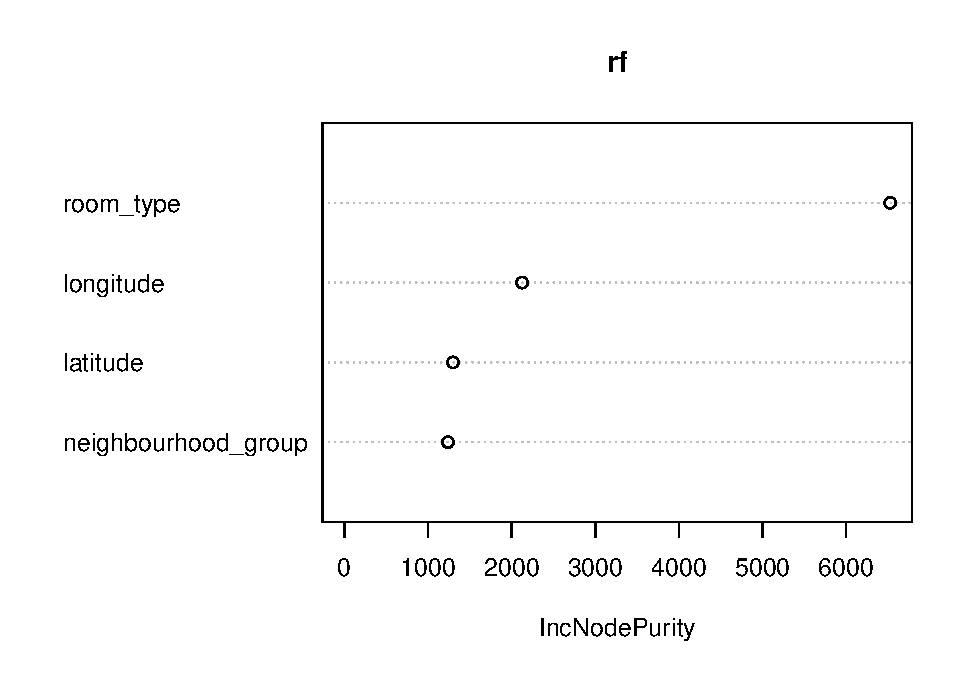
\includegraphics{project_files/figure-latex/unnamed-chunk-18-1.pdf}

\begin{Shaded}
\begin{Highlighting}[]
\KeywordTok{plot}\NormalTok{(rf)}
\end{Highlighting}
\end{Shaded}

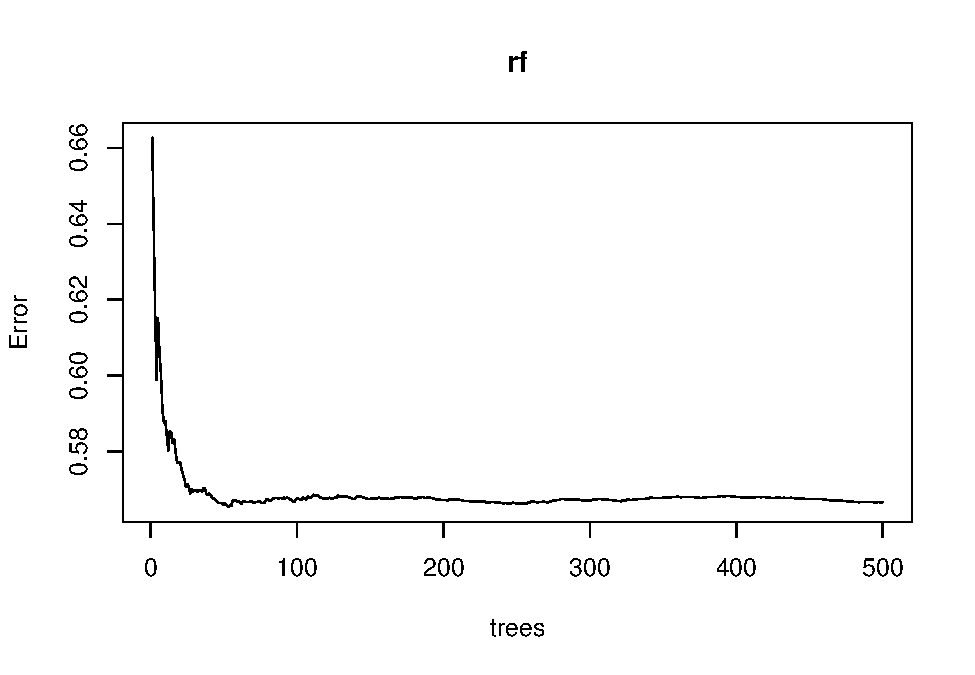
\includegraphics{project_files/figure-latex/unnamed-chunk-18-2.pdf}

\begin{Shaded}
\begin{Highlighting}[]
\KeywordTok{cat}\NormalTok{(}\StringTok{"=== Random Forest selecting the Neighboorhood group and room_type ===}\CharTok{\textbackslash{}n}\StringTok{"}\NormalTok{)}
\end{Highlighting}
\end{Shaded}

\begin{verbatim}
## === Random Forest selecting the Neighboorhood group and room_type ===
\end{verbatim}

\begin{Shaded}
\begin{Highlighting}[]
\KeywordTok{cat}\NormalTok{(}\StringTok{"Neighboorhood group = Manhattan and room_type = Entire home/apt}\CharTok{\textbackslash{}n}\StringTok{ "}\NormalTok{)}
\end{Highlighting}
\end{Shaded}

\begin{verbatim}
## Neighboorhood group = Manhattan and room_type = Entire home/apt
## 
\end{verbatim}

\begin{Shaded}
\begin{Highlighting}[]
\NormalTok{rf2 <-}\StringTok{ }\KeywordTok{randomForest}\NormalTok{(}
\NormalTok{  price }\OperatorTok{~}\StringTok{ }\NormalTok{.,}
  \DataTypeTok{data=}\NormalTok{train_neig,}
  \CommentTok{# importance = TRUE}
\NormalTok{)}
\NormalTok{rf2}
\end{Highlighting}
\end{Shaded}

\begin{verbatim}
## 
## Call:
##  randomForest(formula = price ~ ., data = train_neig, ) 
##                Type of random forest: regression
##                      Number of trees: 500
## No. of variables tried at each split: 1
## 
##           Mean of squared residuals: 0.7191673
##                     % Var explained: 37.83
\end{verbatim}

\begin{Shaded}
\begin{Highlighting}[]
\KeywordTok{varImpPlot}\NormalTok{(rf2)}
\end{Highlighting}
\end{Shaded}

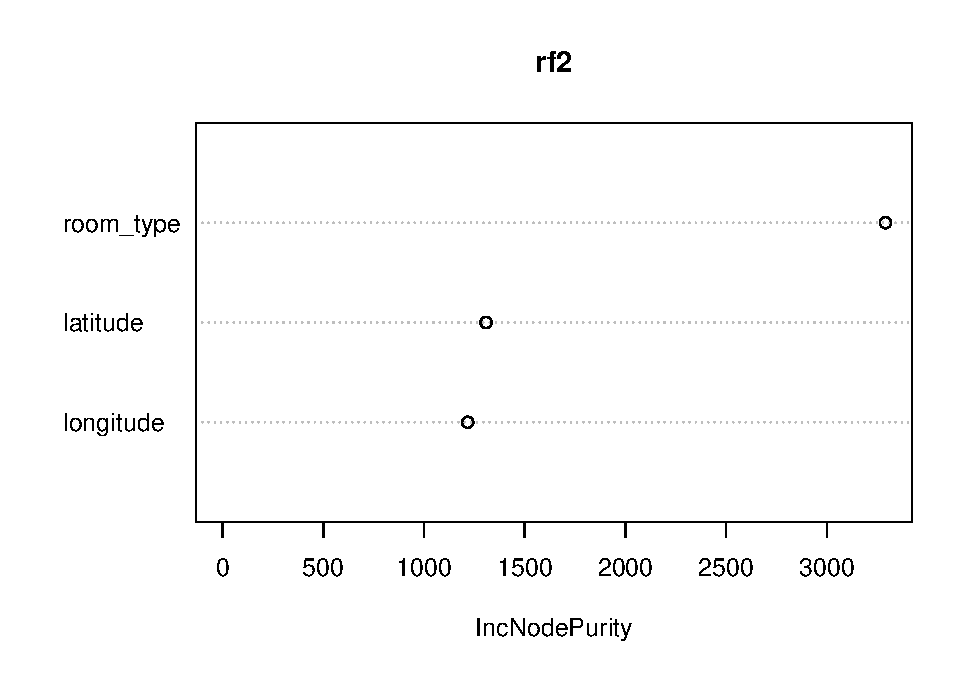
\includegraphics{project_files/figure-latex/unnamed-chunk-19-1.pdf}

\begin{Shaded}
\begin{Highlighting}[]
\KeywordTok{plot}\NormalTok{(rf2)}
\end{Highlighting}
\end{Shaded}

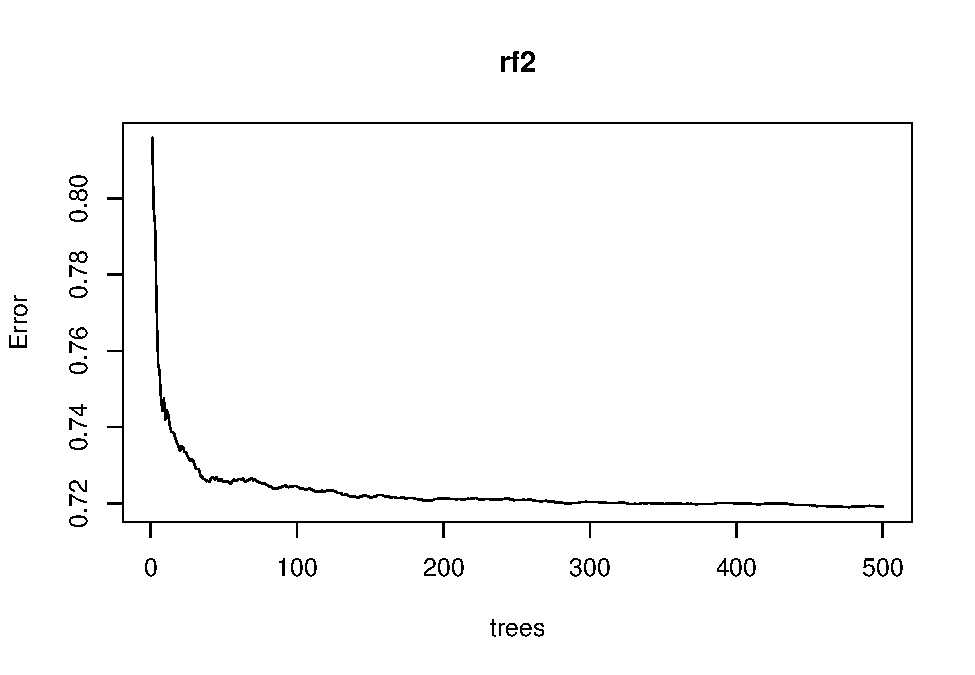
\includegraphics{project_files/figure-latex/unnamed-chunk-19-2.pdf}

\begin{Shaded}
\begin{Highlighting}[]
\KeywordTok{cat}\NormalTok{(}\StringTok{" === Random Forest selecting the Neighboorhood group === }\CharTok{\textbackslash{}n}\StringTok{"}\NormalTok{)}
\end{Highlighting}
\end{Shaded}

\begin{verbatim}
##  === Random Forest selecting the Neighboorhood group ===
\end{verbatim}

\begin{Shaded}
\begin{Highlighting}[]
\KeywordTok{cat}\NormalTok{(}\StringTok{"Neighboorhood group = Manhattan}\CharTok{\textbackslash{}n}\StringTok{ "}\NormalTok{)}
\end{Highlighting}
\end{Shaded}

\begin{verbatim}
## Neighboorhood group = Manhattan
## 
\end{verbatim}

\begin{Shaded}
\begin{Highlighting}[]
\NormalTok{rf3 <-}\StringTok{ }\KeywordTok{randomForest}\NormalTok{(}
\NormalTok{  price }\OperatorTok{~}\StringTok{ }\NormalTok{.,}
  \DataTypeTok{data=}\NormalTok{train_neig_room,}
  \CommentTok{# importance = TRUE}
\NormalTok{)}
\NormalTok{rf3}
\end{Highlighting}
\end{Shaded}

\begin{verbatim}
## 
## Call:
##  randomForest(formula = price ~ ., data = train_neig_room, ) 
##                Type of random forest: regression
##                      Number of trees: 500
## No. of variables tried at each split: 1
## 
##           Mean of squared residuals: 0.3687785
##                     % Var explained: 26.23
\end{verbatim}

\begin{Shaded}
\begin{Highlighting}[]
\KeywordTok{varImpPlot}\NormalTok{(rf3)}
\end{Highlighting}
\end{Shaded}

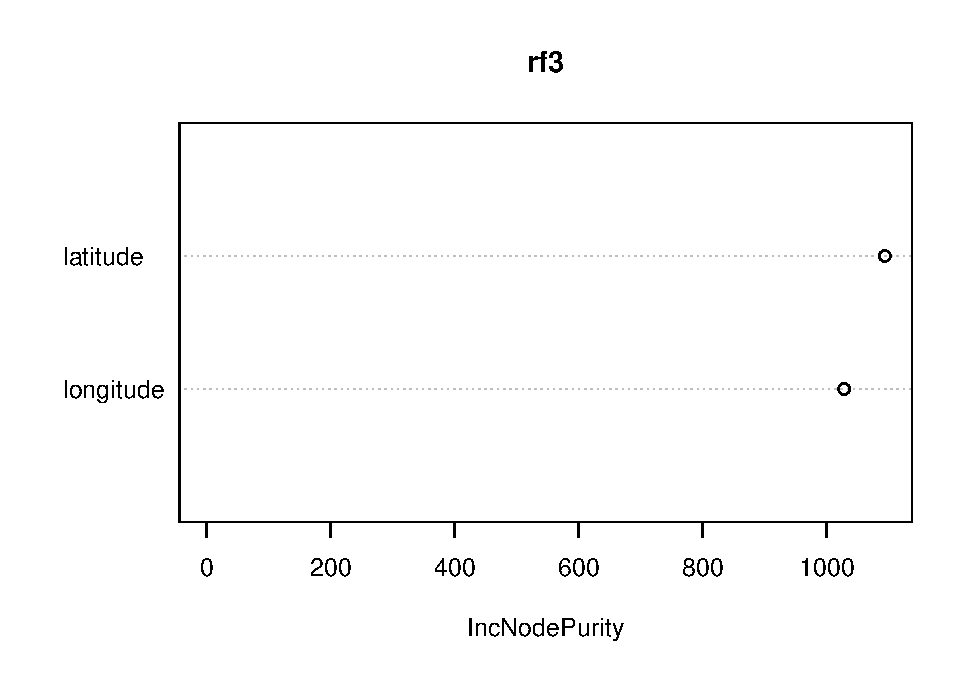
\includegraphics{project_files/figure-latex/unnamed-chunk-20-1.pdf}

\begin{Shaded}
\begin{Highlighting}[]
\KeywordTok{plot}\NormalTok{(rf3)}
\end{Highlighting}
\end{Shaded}

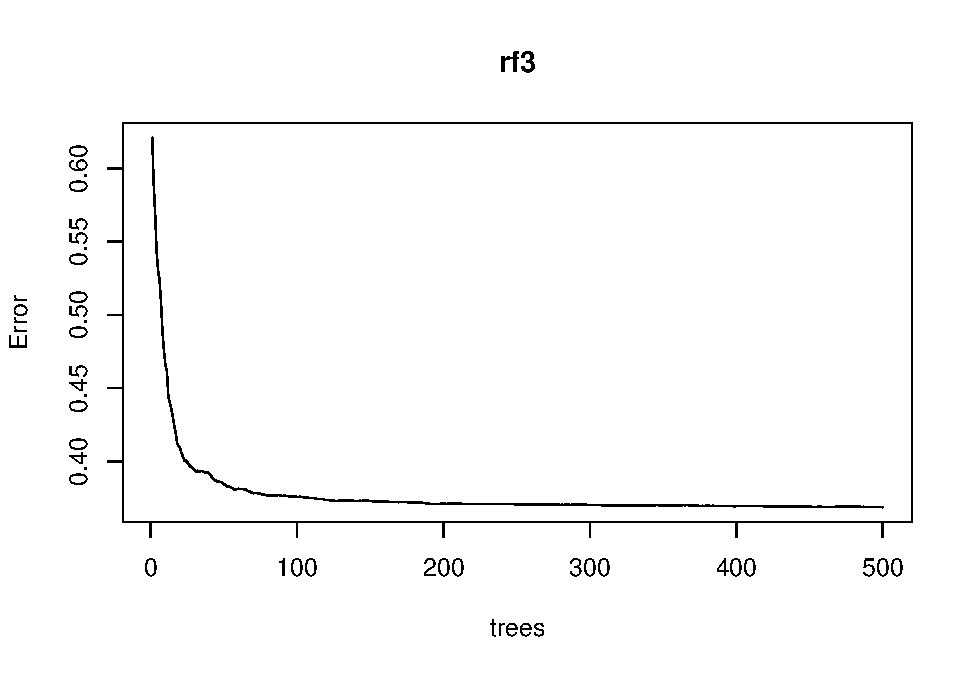
\includegraphics{project_files/figure-latex/unnamed-chunk-20-2.pdf}

\begin{Shaded}
\begin{Highlighting}[]
\KeywordTok{par}\NormalTok{(}\DataTypeTok{mfrow=}\KeywordTok{c}\NormalTok{(}\DecValTok{1}\NormalTok{,}\DecValTok{2}\NormalTok{))}
\KeywordTok{plot}\NormalTok{(test}\OperatorTok{$}\NormalTok{price,}\KeywordTok{predict}\NormalTok{(rf,test),}\DataTypeTok{col=}\StringTok{'red'}\NormalTok{,}\DataTypeTok{main=}\StringTok{'Real vs predicted RF'}\NormalTok{,}\DataTypeTok{pch=}\DecValTok{18}\NormalTok{,}\DataTypeTok{cex=}\FloatTok{0.7}\NormalTok{)}
\KeywordTok{abline}\NormalTok{(}\DecValTok{0}\NormalTok{,}\DecValTok{1}\NormalTok{,}\DataTypeTok{lwd=}\DecValTok{2}\NormalTok{)}
\KeywordTok{legend}\NormalTok{(}\StringTok{'bottomright'}\NormalTok{,}\DataTypeTok{legend=}\StringTok{'NN'}\NormalTok{,}\DataTypeTok{pch=}\DecValTok{18}\NormalTok{,}\DataTypeTok{col=}\StringTok{'red'}\NormalTok{, }\DataTypeTok{bty=}\StringTok{'n'}\NormalTok{)}


\KeywordTok{par}\NormalTok{(}\DataTypeTok{mfrow=}\KeywordTok{c}\NormalTok{(}\DecValTok{1}\NormalTok{,}\DecValTok{2}\NormalTok{))}
\end{Highlighting}
\end{Shaded}

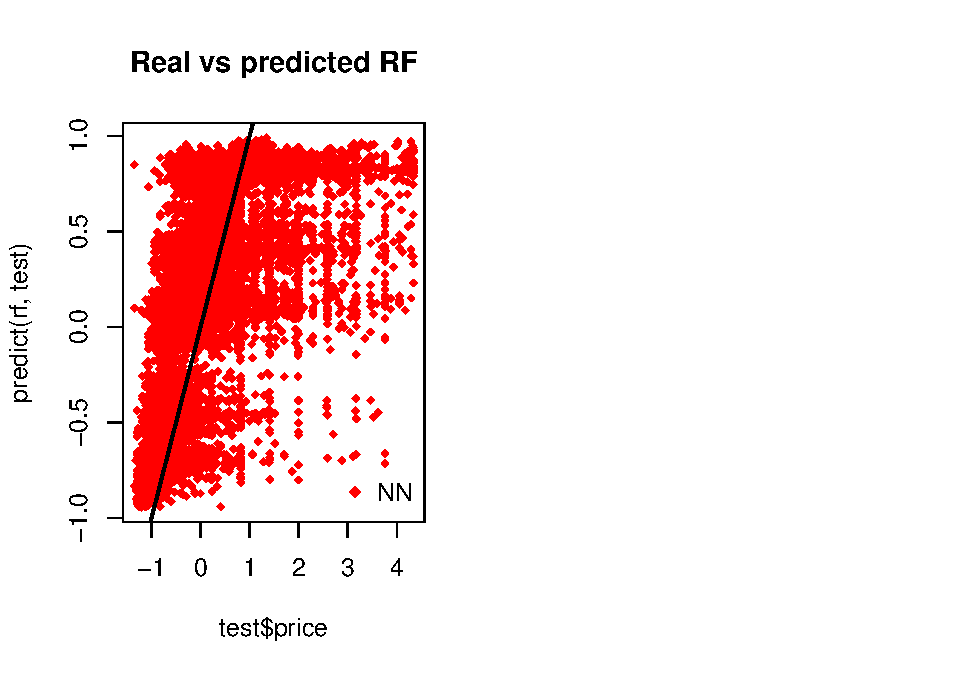
\includegraphics{project_files/figure-latex/unnamed-chunk-21-1.pdf}

\begin{Shaded}
\begin{Highlighting}[]
\KeywordTok{plot}\NormalTok{(train}\OperatorTok{$}\NormalTok{price,}\KeywordTok{predict}\NormalTok{(rf),}\DataTypeTok{col=}\StringTok{'red'}\NormalTok{,}\DataTypeTok{main=}\StringTok{'OOB error'}\NormalTok{,}\DataTypeTok{pch=}\DecValTok{18}\NormalTok{,}\DataTypeTok{cex=}\FloatTok{0.7}\NormalTok{)}
\KeywordTok{abline}\NormalTok{(}\DecValTok{0}\NormalTok{,}\DecValTok{1}\NormalTok{,}\DataTypeTok{lwd=}\DecValTok{2}\NormalTok{)}
\KeywordTok{legend}\NormalTok{(}\StringTok{'bottomright'}\NormalTok{,}\DataTypeTok{legend=}\StringTok{'NN'}\NormalTok{,}\DataTypeTok{pch=}\DecValTok{18}\NormalTok{,}\DataTypeTok{col=}\StringTok{'red'}\NormalTok{, }\DataTypeTok{bty=}\StringTok{'n'}\NormalTok{)}
\end{Highlighting}
\end{Shaded}

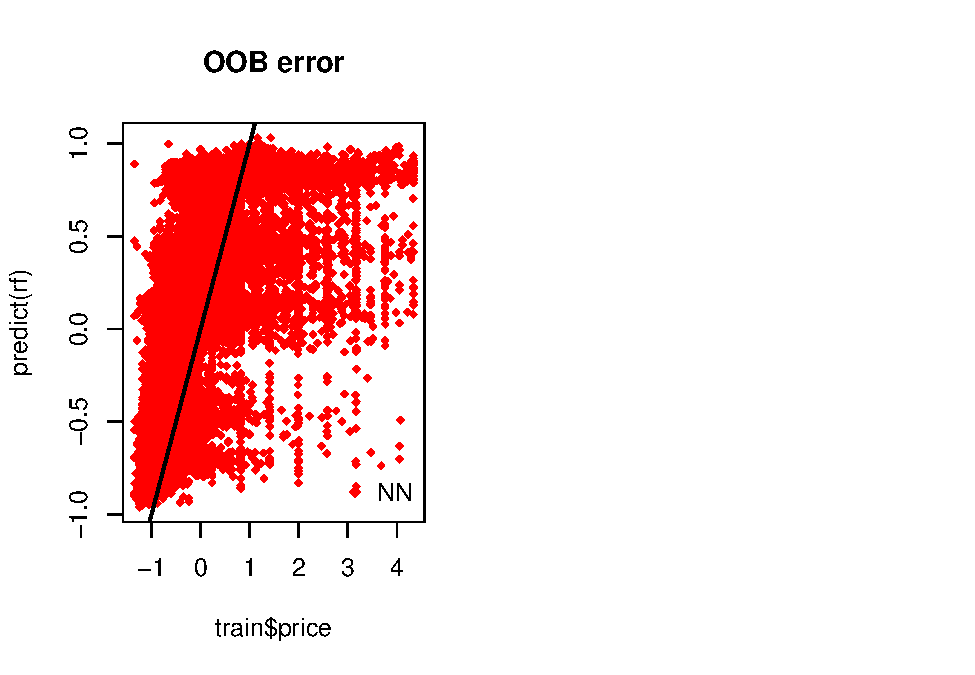
\includegraphics{project_files/figure-latex/unnamed-chunk-21-2.pdf}

\begin{Shaded}
\begin{Highlighting}[]
\NormalTok{pred <-}\KeywordTok{predict}\NormalTok{(rf,test)}
\NormalTok{actuals_preds <-}\StringTok{ }\KeywordTok{data.frame}\NormalTok{(}\KeywordTok{cbind}\NormalTok{(}\DataTypeTok{actuals=}\NormalTok{test}\OperatorTok{$}\NormalTok{price, }\DataTypeTok{predicteds=}\NormalTok{pred))  }\CommentTok{# make actuals_predicteds dataframe.}

\NormalTok{correlation_accuracy <-}\StringTok{ }\KeywordTok{cor}\NormalTok{(actuals_preds)  }\CommentTok{# 0.6043436}
\KeywordTok{print}\NormalTok{(correlation_accuracy)}
\end{Highlighting}
\end{Shaded}

\begin{verbatim}
##              actuals predicteds
## actuals    1.0000000  0.6734816
## predicteds 0.6734816  1.0000000
\end{verbatim}

\begin{Shaded}
\begin{Highlighting}[]
\KeywordTok{head}\NormalTok{(actuals_preds)}
\end{Highlighting}
\end{Shaded}

\begin{verbatim}
##       actuals  predicteds
## 2   1.1152290  0.82245026
## 3   0.2334236 -0.41994376
## 7  -0.8247428 -0.66524979
## 8  -0.6013521  0.07262528
## 12 -0.5308077  0.07695198
## 13 -0.4837781 -0.46915181
\end{verbatim}

\begin{Shaded}
\begin{Highlighting}[]
\NormalTok{min_max_accuracy <-}\StringTok{ }\KeywordTok{mean}\NormalTok{(}\KeywordTok{apply}\NormalTok{(actuals_preds, }\DecValTok{1}\NormalTok{, min) }\OperatorTok{/}\StringTok{ }\KeywordTok{apply}\NormalTok{(actuals_preds, }\DecValTok{1}\NormalTok{, max))  }
\NormalTok{min_max_accuracy}
\end{Highlighting}
\end{Shaded}

\begin{verbatim}
## [1] 0.8444368
\end{verbatim}

\begin{Shaded}
\begin{Highlighting}[]
\NormalTok{mape <-}\StringTok{ }\KeywordTok{mean}\NormalTok{(}\KeywordTok{abs}\NormalTok{((actuals_preds}\OperatorTok{$}\NormalTok{predicteds }\OperatorTok{-}\StringTok{ }\NormalTok{actuals_preds}\OperatorTok{$}\NormalTok{actuals))}\OperatorTok{/}\NormalTok{actuals_preds}\OperatorTok{$}\NormalTok{actuals)}
\NormalTok{mape}
\end{Highlighting}
\end{Shaded}

\begin{verbatim}
## [1] -3.37508
\end{verbatim}

\begin{Shaded}
\begin{Highlighting}[]
\KeywordTok{library}\NormalTok{(randomForest)}
\KeywordTok{library}\NormalTok{(e1071)}
\KeywordTok{library}\NormalTok{(caret)}
\NormalTok{trControl <-}\StringTok{ }\KeywordTok{trainControl}\NormalTok{(}\DataTypeTok{method =} \StringTok{"cv"}\NormalTok{,}
                          \DataTypeTok{number =} \DecValTok{10}\NormalTok{,}
                          \DataTypeTok{search =} \StringTok{"grid"}\NormalTok{,}
                          \DataTypeTok{allowParallel =} \OtherTok{TRUE}
\NormalTok{                        )}
\NormalTok{trControl}\OperatorTok{$}\NormalTok{method}
\end{Highlighting}
\end{Shaded}

\begin{verbatim}
## [1] "cv"
\end{verbatim}

\begin{Shaded}
\begin{Highlighting}[]
\NormalTok{trControl}\OperatorTok{$}\NormalTok{number}
\end{Highlighting}
\end{Shaded}

\begin{verbatim}
## [1] 10
\end{verbatim}

\begin{Shaded}
\begin{Highlighting}[]
\KeywordTok{library}\NormalTok{(doParallel)}
\end{Highlighting}
\end{Shaded}

\begin{verbatim}
## Loading required package: foreach
\end{verbatim}

\begin{verbatim}
## 
## Attaching package: 'foreach'
\end{verbatim}

\begin{verbatim}
## The following objects are masked from 'package:purrr':
## 
##     accumulate, when
\end{verbatim}

\begin{verbatim}
## Loading required package: iterators
\end{verbatim}

\begin{verbatim}
## Loading required package: parallel
\end{verbatim}

\begin{Shaded}
\begin{Highlighting}[]
\KeywordTok{library}\NormalTok{(doFuture)}
\end{Highlighting}
\end{Shaded}

\begin{verbatim}
## Loading required package: globals
\end{verbatim}

\begin{verbatim}
## Loading required package: future
\end{verbatim}

\begin{verbatim}
## 
## Attaching package: 'future'
\end{verbatim}

\begin{verbatim}
## The following object is masked from 'package:caret':
## 
##     cluster
\end{verbatim}

\begin{Shaded}
\begin{Highlighting}[]
\NormalTok{start.time <-}\StringTok{ }\KeywordTok{Sys.time}\NormalTok{()}


\NormalTok{rf_default <-}\StringTok{ }\NormalTok{caret}\OperatorTok{::}\KeywordTok{train}\NormalTok{(}
\NormalTok{  price }\OperatorTok{~}\StringTok{ }\NormalTok{. ,}
  \DataTypeTok{data=}\NormalTok{train_neig_room,}
  \DataTypeTok{method =} \StringTok{"rf"}\NormalTok{,}
  \DataTypeTok{trControl =}\NormalTok{ trControl,}
  \DataTypeTok{num.threads =} \KeywordTok{availableCores}\NormalTok{() }\CommentTok{# <- This one}
  
\NormalTok{)}
\end{Highlighting}
\end{Shaded}

\begin{verbatim}
## note: only 1 unique complexity parameters in default grid. Truncating the grid to 1 .
\end{verbatim}

\begin{Shaded}
\begin{Highlighting}[]
\NormalTok{end.time <-}\StringTok{ }\KeywordTok{Sys.time}\NormalTok{()}
\NormalTok{time.taken <-}\StringTok{ }\NormalTok{end.time }\OperatorTok{-}\StringTok{ }\NormalTok{start.time}

\KeywordTok{print}\NormalTok{(}\StringTok{"-- Time: -- "}\NormalTok{)}
\end{Highlighting}
\end{Shaded}

\begin{verbatim}
## [1] "-- Time: -- "
\end{verbatim}

\begin{Shaded}
\begin{Highlighting}[]
\NormalTok{time.taken}
\end{Highlighting}
\end{Shaded}

\begin{verbatim}
## Time difference of 2.257471 mins
\end{verbatim}

\begin{Shaded}
\begin{Highlighting}[]
\KeywordTok{print}\NormalTok{(}\StringTok{""}\NormalTok{)}
\end{Highlighting}
\end{Shaded}

\begin{verbatim}
## [1] ""
\end{verbatim}

\begin{Shaded}
\begin{Highlighting}[]
\KeywordTok{print}\NormalTok{(}\StringTok{"-- RANDOM FOREST -- "}\NormalTok{)}
\end{Highlighting}
\end{Shaded}

\begin{verbatim}
## [1] "-- RANDOM FOREST -- "
\end{verbatim}

\begin{Shaded}
\begin{Highlighting}[]
\KeywordTok{print}\NormalTok{(rf_default)}
\end{Highlighting}
\end{Shaded}

\begin{verbatim}
## Random Forest 
## 
## 4717 samples
##    2 predictor
## 
## No pre-processing
## Resampling: Cross-Validated (10 fold) 
## Summary of sample sizes: 4246, 4244, 4246, 4246, 4247, 4246, ... 
## Resampling results:
## 
##   RMSE      Rsquared   MAE     
##   0.620016  0.2570873  0.417381
## 
## Tuning parameter 'mtry' was held constant at a value of 2
\end{verbatim}

\begin{Shaded}
\begin{Highlighting}[]
\NormalTok{start.time <-}\StringTok{ }\KeywordTok{Sys.time}\NormalTok{()}

\KeywordTok{set.seed}\NormalTok{(}\DecValTok{1234}\NormalTok{)}
\NormalTok{tuneGrid <-}\StringTok{ }\KeywordTok{expand.grid}\NormalTok{(}\DataTypeTok{.mtry =} \KeywordTok{c}\NormalTok{(}\DecValTok{1}\OperatorTok{:}\StringTok{ }\DecValTok{10}\NormalTok{))}
\NormalTok{rf_mtry <-}\StringTok{ }\NormalTok{caret}\OperatorTok{::}\KeywordTok{train}\NormalTok{(}
\NormalTok{  price}\OperatorTok{~}\NormalTok{.,}
  \DataTypeTok{data =}\NormalTok{ train_neig_room,}
  \DataTypeTok{method =} \StringTok{"rf"}\NormalTok{,}
  \CommentTok{#metric = "Accuracy",}
  \DataTypeTok{tuneGrid =}\NormalTok{ tuneGrid,}
  \DataTypeTok{trControl =}\NormalTok{ trControl,}
  \DataTypeTok{importance =} \OtherTok{TRUE}\NormalTok{,}
  \DataTypeTok{nodesize =} \DecValTok{14}\NormalTok{,}
  \DataTypeTok{ntree =} \DecValTok{300}\NormalTok{,}
  \DataTypeTok{num.threads =} \KeywordTok{availableCores}\NormalTok{()}
\NormalTok{)}
\end{Highlighting}
\end{Shaded}

\begin{verbatim}
## Warning in randomForest.default(x, y, mtry = param$mtry, ...): invalid mtry:
## reset to within valid range

## Warning in randomForest.default(x, y, mtry = param$mtry, ...): invalid mtry:
## reset to within valid range

## Warning in randomForest.default(x, y, mtry = param$mtry, ...): invalid mtry:
## reset to within valid range

## Warning in randomForest.default(x, y, mtry = param$mtry, ...): invalid mtry:
## reset to within valid range

## Warning in randomForest.default(x, y, mtry = param$mtry, ...): invalid mtry:
## reset to within valid range

## Warning in randomForest.default(x, y, mtry = param$mtry, ...): invalid mtry:
## reset to within valid range

## Warning in randomForest.default(x, y, mtry = param$mtry, ...): invalid mtry:
## reset to within valid range

## Warning in randomForest.default(x, y, mtry = param$mtry, ...): invalid mtry:
## reset to within valid range

## Warning in randomForest.default(x, y, mtry = param$mtry, ...): invalid mtry:
## reset to within valid range

## Warning in randomForest.default(x, y, mtry = param$mtry, ...): invalid mtry:
## reset to within valid range

## Warning in randomForest.default(x, y, mtry = param$mtry, ...): invalid mtry:
## reset to within valid range

## Warning in randomForest.default(x, y, mtry = param$mtry, ...): invalid mtry:
## reset to within valid range

## Warning in randomForest.default(x, y, mtry = param$mtry, ...): invalid mtry:
## reset to within valid range

## Warning in randomForest.default(x, y, mtry = param$mtry, ...): invalid mtry:
## reset to within valid range

## Warning in randomForest.default(x, y, mtry = param$mtry, ...): invalid mtry:
## reset to within valid range

## Warning in randomForest.default(x, y, mtry = param$mtry, ...): invalid mtry:
## reset to within valid range

## Warning in randomForest.default(x, y, mtry = param$mtry, ...): invalid mtry:
## reset to within valid range

## Warning in randomForest.default(x, y, mtry = param$mtry, ...): invalid mtry:
## reset to within valid range

## Warning in randomForest.default(x, y, mtry = param$mtry, ...): invalid mtry:
## reset to within valid range

## Warning in randomForest.default(x, y, mtry = param$mtry, ...): invalid mtry:
## reset to within valid range

## Warning in randomForest.default(x, y, mtry = param$mtry, ...): invalid mtry:
## reset to within valid range

## Warning in randomForest.default(x, y, mtry = param$mtry, ...): invalid mtry:
## reset to within valid range

## Warning in randomForest.default(x, y, mtry = param$mtry, ...): invalid mtry:
## reset to within valid range

## Warning in randomForest.default(x, y, mtry = param$mtry, ...): invalid mtry:
## reset to within valid range

## Warning in randomForest.default(x, y, mtry = param$mtry, ...): invalid mtry:
## reset to within valid range

## Warning in randomForest.default(x, y, mtry = param$mtry, ...): invalid mtry:
## reset to within valid range

## Warning in randomForest.default(x, y, mtry = param$mtry, ...): invalid mtry:
## reset to within valid range

## Warning in randomForest.default(x, y, mtry = param$mtry, ...): invalid mtry:
## reset to within valid range

## Warning in randomForest.default(x, y, mtry = param$mtry, ...): invalid mtry:
## reset to within valid range

## Warning in randomForest.default(x, y, mtry = param$mtry, ...): invalid mtry:
## reset to within valid range

## Warning in randomForest.default(x, y, mtry = param$mtry, ...): invalid mtry:
## reset to within valid range

## Warning in randomForest.default(x, y, mtry = param$mtry, ...): invalid mtry:
## reset to within valid range

## Warning in randomForest.default(x, y, mtry = param$mtry, ...): invalid mtry:
## reset to within valid range

## Warning in randomForest.default(x, y, mtry = param$mtry, ...): invalid mtry:
## reset to within valid range

## Warning in randomForest.default(x, y, mtry = param$mtry, ...): invalid mtry:
## reset to within valid range

## Warning in randomForest.default(x, y, mtry = param$mtry, ...): invalid mtry:
## reset to within valid range

## Warning in randomForest.default(x, y, mtry = param$mtry, ...): invalid mtry:
## reset to within valid range

## Warning in randomForest.default(x, y, mtry = param$mtry, ...): invalid mtry:
## reset to within valid range

## Warning in randomForest.default(x, y, mtry = param$mtry, ...): invalid mtry:
## reset to within valid range

## Warning in randomForest.default(x, y, mtry = param$mtry, ...): invalid mtry:
## reset to within valid range

## Warning in randomForest.default(x, y, mtry = param$mtry, ...): invalid mtry:
## reset to within valid range

## Warning in randomForest.default(x, y, mtry = param$mtry, ...): invalid mtry:
## reset to within valid range

## Warning in randomForest.default(x, y, mtry = param$mtry, ...): invalid mtry:
## reset to within valid range

## Warning in randomForest.default(x, y, mtry = param$mtry, ...): invalid mtry:
## reset to within valid range

## Warning in randomForest.default(x, y, mtry = param$mtry, ...): invalid mtry:
## reset to within valid range

## Warning in randomForest.default(x, y, mtry = param$mtry, ...): invalid mtry:
## reset to within valid range

## Warning in randomForest.default(x, y, mtry = param$mtry, ...): invalid mtry:
## reset to within valid range

## Warning in randomForest.default(x, y, mtry = param$mtry, ...): invalid mtry:
## reset to within valid range

## Warning in randomForest.default(x, y, mtry = param$mtry, ...): invalid mtry:
## reset to within valid range

## Warning in randomForest.default(x, y, mtry = param$mtry, ...): invalid mtry:
## reset to within valid range

## Warning in randomForest.default(x, y, mtry = param$mtry, ...): invalid mtry:
## reset to within valid range

## Warning in randomForest.default(x, y, mtry = param$mtry, ...): invalid mtry:
## reset to within valid range

## Warning in randomForest.default(x, y, mtry = param$mtry, ...): invalid mtry:
## reset to within valid range

## Warning in randomForest.default(x, y, mtry = param$mtry, ...): invalid mtry:
## reset to within valid range

## Warning in randomForest.default(x, y, mtry = param$mtry, ...): invalid mtry:
## reset to within valid range

## Warning in randomForest.default(x, y, mtry = param$mtry, ...): invalid mtry:
## reset to within valid range

## Warning in randomForest.default(x, y, mtry = param$mtry, ...): invalid mtry:
## reset to within valid range

## Warning in randomForest.default(x, y, mtry = param$mtry, ...): invalid mtry:
## reset to within valid range

## Warning in randomForest.default(x, y, mtry = param$mtry, ...): invalid mtry:
## reset to within valid range

## Warning in randomForest.default(x, y, mtry = param$mtry, ...): invalid mtry:
## reset to within valid range

## Warning in randomForest.default(x, y, mtry = param$mtry, ...): invalid mtry:
## reset to within valid range

## Warning in randomForest.default(x, y, mtry = param$mtry, ...): invalid mtry:
## reset to within valid range

## Warning in randomForest.default(x, y, mtry = param$mtry, ...): invalid mtry:
## reset to within valid range

## Warning in randomForest.default(x, y, mtry = param$mtry, ...): invalid mtry:
## reset to within valid range

## Warning in randomForest.default(x, y, mtry = param$mtry, ...): invalid mtry:
## reset to within valid range

## Warning in randomForest.default(x, y, mtry = param$mtry, ...): invalid mtry:
## reset to within valid range

## Warning in randomForest.default(x, y, mtry = param$mtry, ...): invalid mtry:
## reset to within valid range

## Warning in randomForest.default(x, y, mtry = param$mtry, ...): invalid mtry:
## reset to within valid range

## Warning in randomForest.default(x, y, mtry = param$mtry, ...): invalid mtry:
## reset to within valid range

## Warning in randomForest.default(x, y, mtry = param$mtry, ...): invalid mtry:
## reset to within valid range

## Warning in randomForest.default(x, y, mtry = param$mtry, ...): invalid mtry:
## reset to within valid range

## Warning in randomForest.default(x, y, mtry = param$mtry, ...): invalid mtry:
## reset to within valid range

## Warning in randomForest.default(x, y, mtry = param$mtry, ...): invalid mtry:
## reset to within valid range

## Warning in randomForest.default(x, y, mtry = param$mtry, ...): invalid mtry:
## reset to within valid range

## Warning in randomForest.default(x, y, mtry = param$mtry, ...): invalid mtry:
## reset to within valid range

## Warning in randomForest.default(x, y, mtry = param$mtry, ...): invalid mtry:
## reset to within valid range

## Warning in randomForest.default(x, y, mtry = param$mtry, ...): invalid mtry:
## reset to within valid range

## Warning in randomForest.default(x, y, mtry = param$mtry, ...): invalid mtry:
## reset to within valid range

## Warning in randomForest.default(x, y, mtry = param$mtry, ...): invalid mtry:
## reset to within valid range

## Warning in randomForest.default(x, y, mtry = param$mtry, ...): invalid mtry:
## reset to within valid range
\end{verbatim}

\begin{Shaded}
\begin{Highlighting}[]
\NormalTok{end.time <-}\StringTok{ }\KeywordTok{Sys.time}\NormalTok{()}
\NormalTok{time.taken <-}\StringTok{ }\NormalTok{end.time }\OperatorTok{-}\StringTok{ }\NormalTok{start.time}

\KeywordTok{print}\NormalTok{(}\StringTok{"-- Time: -- "}\NormalTok{)}
\end{Highlighting}
\end{Shaded}

\begin{verbatim}
## [1] "-- Time: -- "
\end{verbatim}

\begin{Shaded}
\begin{Highlighting}[]
\NormalTok{time.taken}
\end{Highlighting}
\end{Shaded}

\begin{verbatim}
## Time difference of 7.874638 mins
\end{verbatim}

\begin{Shaded}
\begin{Highlighting}[]
\KeywordTok{print}\NormalTok{(}\StringTok{""}\NormalTok{)}
\end{Highlighting}
\end{Shaded}

\begin{verbatim}
## [1] ""
\end{verbatim}

\begin{Shaded}
\begin{Highlighting}[]
\KeywordTok{print}\NormalTok{(rf_mtry)}
\end{Highlighting}
\end{Shaded}

\begin{verbatim}
## Random Forest 
## 
## 4717 samples
##    2 predictor
## 
## No pre-processing
## Resampling: Cross-Validated (10 fold) 
## Summary of sample sizes: 4247, 4246, 4243, 4247, 4244, 4245, ... 
## Resampling results across tuning parameters:
## 
##   mtry  RMSE       Rsquared   MAE      
##    1    0.5990288  0.2840629  0.4040160
##    2    0.6032310  0.2798206  0.4075759
##    3    0.6029938  0.2805047  0.4073863
##    4    0.6031070  0.2802278  0.4078976
##    5    0.6020111  0.2822330  0.4076411
##    6    0.6029198  0.2802763  0.4078772
##    7    0.6036097  0.2793002  0.4080061
##    8    0.6015838  0.2831863  0.4073911
##    9    0.6025460  0.2811281  0.4075416
##   10    0.6028483  0.2807578  0.4077423
## 
## RMSE was used to select the optimal model using the smallest value.
## The final value used for the model was mtry = 1.
\end{verbatim}

\begin{Shaded}
\begin{Highlighting}[]
\NormalTok{best_mtry <-}\StringTok{ }\NormalTok{rf_mtry}\OperatorTok{$}\NormalTok{bestTune}\OperatorTok{$}\NormalTok{mtry }
\KeywordTok{cat}\NormalTok{(}\StringTok{"Best mtry value:"}\NormalTok{,best_mtry)}
\end{Highlighting}
\end{Shaded}

\begin{verbatim}
## Best mtry value: 1
\end{verbatim}

\begin{Shaded}
\begin{Highlighting}[]
\KeywordTok{cat}\NormalTok{(}\StringTok{"}\CharTok{\textbackslash{}n}\StringTok{Max accuracy mtry:"}\NormalTok{, }\KeywordTok{max}\NormalTok{(rf_mtry}\OperatorTok{$}\NormalTok{results}\OperatorTok{$}\NormalTok{Accuracy))}
\end{Highlighting}
\end{Shaded}

\begin{verbatim}
## Warning in max(rf_mtry$results$Accuracy): no non-missing arguments to max;
## returning -Inf
\end{verbatim}

\begin{verbatim}
## 
## Max accuracy mtry: -Inf
\end{verbatim}

\begin{Shaded}
\begin{Highlighting}[]
\NormalTok{start.time <-}\StringTok{ }\KeywordTok{Sys.time}\NormalTok{()}

\NormalTok{store_maxnode <-}\StringTok{ }\KeywordTok{list}\NormalTok{()}
\NormalTok{tuneGrid <-}\StringTok{ }\KeywordTok{expand.grid}\NormalTok{(}\DataTypeTok{.mtry =}\NormalTok{ best_mtry)}
\ControlFlowTok{for}\NormalTok{ (maxnodes }\ControlFlowTok{in} \KeywordTok{c}\NormalTok{(}\DecValTok{5}\OperatorTok{:}\StringTok{ }\DecValTok{15}\NormalTok{)) \{}
  \KeywordTok{set.seed}\NormalTok{(}\DecValTok{1234}\NormalTok{)}
\NormalTok{  rf_maxnode <-}\StringTok{ }\NormalTok{caret}\OperatorTok{::}\KeywordTok{train}\NormalTok{(price}\OperatorTok{~}\NormalTok{.,}
                      \DataTypeTok{data =}\NormalTok{ train_neig_room,}
                      \DataTypeTok{method =} \StringTok{"rf"}\NormalTok{,}
                      \CommentTok{#metric = "Accuracy",}
                      \DataTypeTok{tuneGrid =}\NormalTok{ tuneGrid,}
                      \DataTypeTok{trControl =}\NormalTok{ trControl,}
                      \DataTypeTok{importance =} \OtherTok{TRUE}\NormalTok{,}
                      \DataTypeTok{nodesize =} \DecValTok{14}\NormalTok{,}
                      \DataTypeTok{maxnodes =}\NormalTok{ maxnodes,}
                      \DataTypeTok{ntree =} \DecValTok{300}\NormalTok{,}
\NormalTok{  )}
\NormalTok{  current_iteration <-}\StringTok{ }\KeywordTok{toString}\NormalTok{(maxnodes)}
\NormalTok{  store_maxnode[[current_iteration]] <-}\StringTok{ }\NormalTok{rf_maxnode}
\NormalTok{\}}

\NormalTok{end.time <-}\StringTok{ }\KeywordTok{Sys.time}\NormalTok{()}
\NormalTok{time.taken <-}\StringTok{ }\NormalTok{end.time }\OperatorTok{-}\StringTok{ }\NormalTok{start.time}

\KeywordTok{print}\NormalTok{(}\StringTok{"-- Time: -- "}\NormalTok{)}
\end{Highlighting}
\end{Shaded}

\begin{verbatim}
## [1] "-- Time: -- "
\end{verbatim}

\begin{Shaded}
\begin{Highlighting}[]
\NormalTok{time.taken}
\end{Highlighting}
\end{Shaded}

\begin{verbatim}
## Time difference of 1.247651 mins
\end{verbatim}

\begin{Shaded}
\begin{Highlighting}[]
\KeywordTok{print}\NormalTok{(}\StringTok{""}\NormalTok{)}
\end{Highlighting}
\end{Shaded}

\begin{verbatim}
## [1] ""
\end{verbatim}

\begin{Shaded}
\begin{Highlighting}[]
\NormalTok{results_mtry <-}\StringTok{ }\KeywordTok{resamples}\NormalTok{(store_maxnode)}
\KeywordTok{summary}\NormalTok{(results_mtry)}
\end{Highlighting}
\end{Shaded}

\begin{verbatim}
## 
## Call:
## summary.resamples(object = results_mtry)
## 
## Models: 5, 6, 7, 8, 9, 10, 11, 12, 13, 14, 15 
## Number of resamples: 10 
## 
## MAE 
##         Min.   1st Qu.    Median      Mean   3rd Qu.      Max. NA's
## 5  0.3684582 0.4062136 0.4129675 0.4160256 0.4293124 0.4616794    0
## 6  0.3670461 0.4047761 0.4109991 0.4141051 0.4273659 0.4583586    0
## 7  0.3688109 0.4039806 0.4108196 0.4141797 0.4269574 0.4596341    0
## 8  0.3673954 0.4021941 0.4114436 0.4133648 0.4267071 0.4586242    0
## 9  0.3665610 0.4013312 0.4115176 0.4129789 0.4263355 0.4587397    0
## 10 0.3660150 0.3986749 0.4101067 0.4110842 0.4245095 0.4566621    0
## 11 0.3651931 0.3953669 0.4085316 0.4096210 0.4239356 0.4555920    0
## 12 0.3670413 0.3951996 0.4083730 0.4093175 0.4234488 0.4548174    0
## 13 0.3663165 0.3957381 0.4088116 0.4094939 0.4229725 0.4542741    0
## 14 0.3666462 0.3945890 0.4087715 0.4093705 0.4223508 0.4554178    0
## 15 0.3664606 0.3939492 0.4081074 0.4086645 0.4221002 0.4548197    0
## 
## RMSE 
##         Min.   1st Qu.    Median      Mean   3rd Qu.      Max. NA's
## 5  0.5098404 0.6199714 0.6262818 0.6334632 0.6737586 0.7066414    0
## 6  0.5096703 0.6158769 0.6208161 0.6291541 0.6702445 0.7031436    0
## 7  0.5115140 0.6157049 0.6205495 0.6290705 0.6694010 0.7029296    0
## 8  0.5110954 0.6144522 0.6217804 0.6287734 0.6699057 0.7028503    0
## 9  0.5105308 0.6140686 0.6224264 0.6282713 0.6686847 0.7016021    0
## 10 0.5095604 0.6110689 0.6196216 0.6250384 0.6661296 0.6979183    0
## 11 0.5110861 0.6087131 0.6150524 0.6215976 0.6635825 0.6963890    0
## 12 0.5124407 0.6046791 0.6148156 0.6199597 0.6626292 0.6942299    0
## 13 0.5111125 0.6049455 0.6155114 0.6205018 0.6629056 0.6943627    0
## 14 0.5127013 0.6053026 0.6149113 0.6206596 0.6619567 0.6960489    0
## 15 0.5122565 0.6039939 0.6141815 0.6197369 0.6616598 0.6947566    0
## 
## Rsquared 
##         Min.   1st Qu.    Median      Mean   3rd Qu.      Max. NA's
## 5  0.1420339 0.1855682 0.1992231 0.1985338 0.2062099 0.2555966    0
## 6  0.1509850 0.1912405 0.2118829 0.2094725 0.2195240 0.2699392    0
## 7  0.1511365 0.1879217 0.2124891 0.2089156 0.2170975 0.2709747    0
## 8  0.1513087 0.1876798 0.2152061 0.2094414 0.2192887 0.2701228    0
## 9  0.1541920 0.1877424 0.2142451 0.2103562 0.2197024 0.2773768    0
## 10 0.1634291 0.1924502 0.2220950 0.2188358 0.2324464 0.2890141    0
## 11 0.1672171 0.1942003 0.2321220 0.2280938 0.2454324 0.3127833    0
## 12 0.1725098 0.1948307 0.2358154 0.2320944 0.2517099 0.3169619    0
## 13 0.1723009 0.1940385 0.2331714 0.2304442 0.2500001 0.3133850    0
## 14 0.1678145 0.1971979 0.2313610 0.2299299 0.2494775 0.3117681    0
## 15 0.1712585 0.1964233 0.2344155 0.2322262 0.2525277 0.3179781    0
\end{verbatim}

\begin{Shaded}
\begin{Highlighting}[]
\NormalTok{start.time <-}\StringTok{ }\KeywordTok{Sys.time}\NormalTok{()}

\ControlFlowTok{for}\NormalTok{ (maxnodes }\ControlFlowTok{in} \KeywordTok{c}\NormalTok{(}\DecValTok{15} \OperatorTok{:}\StringTok{ }\DecValTok{30}\NormalTok{)) \{}
  \KeywordTok{set.seed}\NormalTok{(}\DecValTok{1234}\NormalTok{)}
\NormalTok{  rf_maxnode <-}\StringTok{ }\NormalTok{caret}\OperatorTok{::}\KeywordTok{train}\NormalTok{(price}\OperatorTok{~}\NormalTok{.,}
                      \DataTypeTok{data =}\NormalTok{ train_neig_room,}
                      \DataTypeTok{method =} \StringTok{"rf"}\NormalTok{,}
                     \CommentTok{# metric = "Accuracy",}
                      \DataTypeTok{tuneGrid =}\NormalTok{ tuneGrid,}
                      \DataTypeTok{trControl =}\NormalTok{ trControl,}
                      \DataTypeTok{importance =} \OtherTok{TRUE}\NormalTok{,}
                      \DataTypeTok{nodesize =} \DecValTok{14}\NormalTok{,}
                      \DataTypeTok{maxnodes =}\NormalTok{ maxnodes,}
                      \DataTypeTok{ntree =} \DecValTok{300}\NormalTok{)}
\NormalTok{  current_iteration <-}\StringTok{ }\KeywordTok{toString}\NormalTok{(maxnodes)}
\NormalTok{  store_maxnode[[current_iteration]] <-}\StringTok{ }\NormalTok{rf_maxnode}
\NormalTok{\}}

\NormalTok{end.time <-}\StringTok{ }\KeywordTok{Sys.time}\NormalTok{()}
\NormalTok{time.taken <-}\StringTok{ }\NormalTok{end.time }\OperatorTok{-}\StringTok{ }\NormalTok{start.time}

\KeywordTok{print}\NormalTok{(}\StringTok{"-- Time: -- "}\NormalTok{)}
\end{Highlighting}
\end{Shaded}

\begin{verbatim}
## [1] "-- Time: -- "
\end{verbatim}

\begin{Shaded}
\begin{Highlighting}[]
\NormalTok{time.taken}
\end{Highlighting}
\end{Shaded}

\begin{verbatim}
## Time difference of 2.311585 mins
\end{verbatim}

\begin{Shaded}
\begin{Highlighting}[]
\KeywordTok{print}\NormalTok{(}\StringTok{""}\NormalTok{)}
\end{Highlighting}
\end{Shaded}

\begin{verbatim}
## [1] ""
\end{verbatim}

\begin{Shaded}
\begin{Highlighting}[]
\NormalTok{results_mtry <-}\StringTok{ }\KeywordTok{resamples}\NormalTok{(store_maxnode)}
\KeywordTok{summary}\NormalTok{(results_mtry)}
\end{Highlighting}
\end{Shaded}

\begin{verbatim}
## 
## Call:
## summary.resamples(object = results_mtry)
## 
## Models: 5, 6, 7, 8, 9, 10, 11, 12, 13, 14, 15, 16, 17, 18, 19, 20, 21, 22, 23, 24, 25, 26, 27, 28, 29, 30 
## Number of resamples: 10 
## 
## MAE 
##         Min.   1st Qu.    Median      Mean   3rd Qu.      Max. NA's
## 5  0.3684582 0.4062136 0.4129675 0.4160256 0.4293124 0.4616794    0
## 6  0.3670461 0.4047761 0.4109991 0.4141051 0.4273659 0.4583586    0
## 7  0.3688109 0.4039806 0.4108196 0.4141797 0.4269574 0.4596341    0
## 8  0.3673954 0.4021941 0.4114436 0.4133648 0.4267071 0.4586242    0
## 9  0.3665610 0.4013312 0.4115176 0.4129789 0.4263355 0.4587397    0
## 10 0.3660150 0.3986749 0.4101067 0.4110842 0.4245095 0.4566621    0
## 11 0.3651931 0.3953669 0.4085316 0.4096210 0.4239356 0.4555920    0
## 12 0.3670413 0.3951996 0.4083730 0.4093175 0.4234488 0.4548174    0
## 13 0.3663165 0.3957381 0.4088116 0.4094939 0.4229725 0.4542741    0
## 14 0.3666462 0.3945890 0.4087715 0.4093705 0.4223508 0.4554178    0
## 15 0.3664606 0.3939492 0.4081074 0.4086645 0.4221002 0.4548197    0
## 16 0.3656206 0.3927326 0.4090010 0.4083212 0.4222523 0.4545334    0
## 17 0.3662240 0.3922701 0.4085057 0.4079028 0.4219301 0.4533215    0
## 18 0.3650755 0.3912411 0.4080871 0.4072464 0.4218023 0.4530474    0
## 19 0.3651572 0.3896895 0.4081639 0.4065044 0.4206572 0.4521838    0
## 20 0.3647242 0.3878471 0.4066818 0.4055169 0.4200477 0.4510017    0
## 21 0.3643820 0.3880231 0.4060352 0.4049845 0.4199640 0.4503625    0
## 22 0.3635408 0.3872859 0.4051918 0.4043354 0.4185687 0.4495566    0
## 23 0.3648898 0.3871370 0.4053874 0.4042163 0.4176592 0.4491849    0
## 24 0.3642830 0.3871919 0.4053597 0.4041074 0.4176431 0.4489561    0
## 25 0.3649796 0.3869348 0.4057699 0.4039726 0.4168233 0.4495211    0
## 26 0.3638270 0.3872346 0.4050680 0.4041746 0.4170917 0.4504911    0
## 27 0.3637427 0.3865728 0.4046237 0.4035576 0.4179639 0.4486568    0
## 28 0.3636577 0.3871555 0.4047590 0.4034968 0.4174664 0.4490561    0
## 29 0.3640187 0.3870199 0.4041461 0.4034398 0.4168680 0.4498850    0
## 30 0.3643711 0.3866133 0.4045679 0.4029356 0.4158001 0.4479393    0
## 
## RMSE 
##         Min.   1st Qu.    Median      Mean   3rd Qu.      Max. NA's
## 5  0.5098404 0.6199714 0.6262818 0.6334632 0.6737586 0.7066414    0
## 6  0.5096703 0.6158769 0.6208161 0.6291541 0.6702445 0.7031436    0
## 7  0.5115140 0.6157049 0.6205495 0.6290705 0.6694010 0.7029296    0
## 8  0.5110954 0.6144522 0.6217804 0.6287734 0.6699057 0.7028503    0
## 9  0.5105308 0.6140686 0.6224264 0.6282713 0.6686847 0.7016021    0
## 10 0.5095604 0.6110689 0.6196216 0.6250384 0.6661296 0.6979183    0
## 11 0.5110861 0.6087131 0.6150524 0.6215976 0.6635825 0.6963890    0
## 12 0.5124407 0.6046791 0.6148156 0.6199597 0.6626292 0.6942299    0
## 13 0.5111125 0.6049455 0.6155114 0.6205018 0.6629056 0.6943627    0
## 14 0.5127013 0.6053026 0.6149113 0.6206596 0.6619567 0.6960489    0
## 15 0.5122565 0.6039939 0.6141815 0.6197369 0.6616598 0.6947566    0
## 16 0.5109460 0.6032588 0.6158998 0.6189571 0.6607049 0.6947540    0
## 17 0.5118059 0.6017436 0.6149095 0.6183251 0.6608665 0.6921189    0
## 18 0.5112948 0.6016034 0.6144766 0.6173818 0.6599857 0.6917146    0
## 19 0.5118979 0.6002211 0.6133001 0.6159165 0.6580310 0.6903052    0
## 20 0.5116859 0.5966664 0.6112621 0.6137674 0.6570637 0.6886186    0
## 21 0.5119875 0.5946562 0.6084213 0.6121384 0.6558471 0.6870811    0
## 22 0.5117709 0.5928282 0.6067931 0.6108487 0.6545050 0.6865687    0
## 23 0.5120098 0.5937716 0.6060428 0.6104936 0.6536428 0.6855278    0
## 24 0.5120531 0.5930181 0.6042348 0.6102612 0.6545604 0.6860934    0
## 25 0.5123668 0.5916521 0.6052994 0.6099067 0.6528756 0.6863239    0
## 26 0.5120134 0.5932595 0.6057455 0.6101882 0.6527935 0.6867802    0
## 27 0.5114353 0.5924201 0.6048072 0.6095799 0.6537654 0.6852555    0
## 28 0.5119658 0.5910359 0.6036366 0.6095507 0.6537189 0.6866094    0
## 29 0.5125402 0.5908643 0.6037807 0.6095276 0.6534058 0.6860857    0
## 30 0.5119823 0.5903578 0.6025329 0.6085577 0.6528059 0.6847231    0
## 
## Rsquared 
##         Min.   1st Qu.    Median      Mean   3rd Qu.      Max. NA's
## 5  0.1420339 0.1855682 0.1992231 0.1985338 0.2062099 0.2555966    0
## 6  0.1509850 0.1912405 0.2118829 0.2094725 0.2195240 0.2699392    0
## 7  0.1511365 0.1879217 0.2124891 0.2089156 0.2170975 0.2709747    0
## 8  0.1513087 0.1876798 0.2152061 0.2094414 0.2192887 0.2701228    0
## 9  0.1541920 0.1877424 0.2142451 0.2103562 0.2197024 0.2773768    0
## 10 0.1634291 0.1924502 0.2220950 0.2188358 0.2324464 0.2890141    0
## 11 0.1672171 0.1942003 0.2321220 0.2280938 0.2454324 0.3127833    0
## 12 0.1725098 0.1948307 0.2358154 0.2320944 0.2517099 0.3169619    0
## 13 0.1723009 0.1940385 0.2331714 0.2304442 0.2500001 0.3133850    0
## 14 0.1678145 0.1971979 0.2313610 0.2299299 0.2494775 0.3117681    0
## 15 0.1712585 0.1964233 0.2344155 0.2322262 0.2525277 0.3179781    0
## 16 0.1709162 0.1943547 0.2359221 0.2342261 0.2553969 0.3293401    0
## 17 0.1775499 0.1975954 0.2381160 0.2356636 0.2602962 0.3193528    0
## 18 0.1785839 0.1973250 0.2381266 0.2380267 0.2614589 0.3309694    0
## 19 0.1817568 0.2009271 0.2451704 0.2417820 0.2664981 0.3371487    0
## 20 0.1860431 0.2024807 0.2482733 0.2473047 0.2759033 0.3464677    0
## 21 0.1852355 0.2037093 0.2566254 0.2512804 0.2789398 0.3581412    0
## 22 0.1861423 0.2069613 0.2543492 0.2544516 0.2849340 0.3672185    0
## 23 0.1847899 0.2090570 0.2585692 0.2552824 0.2846170 0.3674314    0
## 24 0.1860419 0.2065384 0.2613711 0.2558012 0.2853251 0.3703108    0
## 25 0.1852360 0.2108741 0.2601882 0.2566263 0.2877932 0.3709559    0
## 26 0.1853245 0.2113271 0.2590212 0.2557498 0.2873045 0.3667349    0
## 27 0.1881028 0.2089011 0.2614841 0.2574326 0.2877881 0.3715194    0
## 28 0.1860840 0.2088407 0.2645325 0.2574824 0.2870826 0.3732101    0
## 29 0.1850631 0.2097374 0.2609407 0.2573416 0.2890308 0.3722731    0
## 30 0.1867006 0.2110420 0.2658184 0.2597242 0.2904218 0.3767907    0
\end{verbatim}

Result: 30

\hypertarget{step-4-search-the-best-ntrees}{%
\subsection{Step 4) Search the best
ntrees}\label{step-4-search-the-best-ntrees}}

Now that you have the best value of mtry and maxnode, you can tune the
number of trees. The method is exactly the same as maxnode.

\begin{Shaded}
\begin{Highlighting}[]
\NormalTok{start.time <-}\StringTok{ }\KeywordTok{Sys.time}\NormalTok{()}

\NormalTok{store_maxtrees <-}\StringTok{ }\KeywordTok{list}\NormalTok{()}
\ControlFlowTok{for}\NormalTok{ (ntree }\ControlFlowTok{in} \KeywordTok{c}\NormalTok{(}\DecValTok{250}\NormalTok{, }\DecValTok{300}\NormalTok{, }\DecValTok{350}\NormalTok{, }\DecValTok{400}\NormalTok{, }\DecValTok{450}\NormalTok{, }\DecValTok{500}\NormalTok{, }\DecValTok{550}\NormalTok{, }\DecValTok{600}\NormalTok{, }\DecValTok{800}\NormalTok{, }\DecValTok{1000}\NormalTok{, }\DecValTok{2000}\NormalTok{)) \{}
  \KeywordTok{set.seed}\NormalTok{(}\DecValTok{5678}\NormalTok{)}
\NormalTok{  rf_maxtrees <-}\StringTok{ }\NormalTok{caret}\OperatorTok{::}\KeywordTok{train}\NormalTok{(price}\OperatorTok{~}\NormalTok{.,}
                       \DataTypeTok{data =}\NormalTok{ train_neig_room,}
                       \DataTypeTok{method =} \StringTok{"rf"}\NormalTok{,}
                       \DataTypeTok{tuneGrid =}\NormalTok{ tuneGrid,}
                       \DataTypeTok{trControl =}\NormalTok{ trControl,}
                      \CommentTok{# importance = TRUE,}
                       \DataTypeTok{nodesize =} \DecValTok{14}\NormalTok{,}
                       \DataTypeTok{maxnodes =} \DecValTok{23}\NormalTok{,}
                       \DataTypeTok{ntree =}\NormalTok{ ntree)}
\NormalTok{  key <-}\StringTok{ }\KeywordTok{toString}\NormalTok{(ntree)}
\NormalTok{  store_maxtrees[[key]] <-}\StringTok{ }\NormalTok{rf_maxtrees}
\NormalTok{\}}

\NormalTok{end.time <-}\StringTok{ }\KeywordTok{Sys.time}\NormalTok{()}
\NormalTok{time.taken <-}\StringTok{ }\NormalTok{end.time }\OperatorTok{-}\StringTok{ }\NormalTok{start.time}

\KeywordTok{print}\NormalTok{(}\StringTok{"-- Time: -- "}\NormalTok{)}
\end{Highlighting}
\end{Shaded}

\begin{verbatim}
## [1] "-- Time: -- "
\end{verbatim}

\begin{Shaded}
\begin{Highlighting}[]
\NormalTok{time.taken}
\end{Highlighting}
\end{Shaded}

\begin{verbatim}
## Time difference of 2.832029 mins
\end{verbatim}

\begin{Shaded}
\begin{Highlighting}[]
\KeywordTok{print}\NormalTok{(}\StringTok{""}\NormalTok{)                                                          }
\end{Highlighting}
\end{Shaded}

\begin{verbatim}
## [1] ""
\end{verbatim}

\begin{Shaded}
\begin{Highlighting}[]
\NormalTok{results_tree <-}\StringTok{ }\KeywordTok{resamples}\NormalTok{(store_maxtrees)}
\KeywordTok{summary}\NormalTok{(results_tree)}
\end{Highlighting}
\end{Shaded}

\begin{verbatim}
## 
## Call:
## summary.resamples(object = results_tree)
## 
## Models: 250, 300, 350, 400, 450, 500, 550, 600, 800, 1000, 2000 
## Number of resamples: 10 
## 
## MAE 
##           Min.   1st Qu.    Median      Mean   3rd Qu.      Max. NA's
## 250  0.3839302 0.3943710 0.3982668 0.4040096 0.4159051 0.4345377    0
## 300  0.3841171 0.3942265 0.3985523 0.4041700 0.4163617 0.4348485    0
## 350  0.3838682 0.3942326 0.3986756 0.4040933 0.4163590 0.4346922    0
## 400  0.3834900 0.3940142 0.3986417 0.4040720 0.4164204 0.4349652    0
## 450  0.3829263 0.3940305 0.3986902 0.4040529 0.4164447 0.4350674    0
## 500  0.3827450 0.3942020 0.3985878 0.4040377 0.4166542 0.4349240    0
## 550  0.3825898 0.3940684 0.3986553 0.4040313 0.4166541 0.4351006    0
## 600  0.3826346 0.3942156 0.3986659 0.4040869 0.4167735 0.4352565    0
## 800  0.3829250 0.3939886 0.3986161 0.4041579 0.4170329 0.4352856    0
## 1000 0.3831445 0.3940886 0.3986175 0.4041620 0.4168747 0.4353121    0
## 2000 0.3828952 0.3941557 0.3987563 0.4041005 0.4167838 0.4351601    0
## 
## RMSE 
##           Min.   1st Qu.    Median      Mean   3rd Qu.      Max. NA's
## 250  0.5723113 0.5865639 0.6043270 0.6107769 0.6210309 0.6808563    0
## 300  0.5720814 0.5870377 0.6042067 0.6107632 0.6213357 0.6800908    0
## 350  0.5715817 0.5871119 0.6040143 0.6107339 0.6213950 0.6803562    0
## 400  0.5714090 0.5869830 0.6040970 0.6108395 0.6216883 0.6805037    0
## 450  0.5716223 0.5865622 0.6040568 0.6109324 0.6218955 0.6807658    0
## 500  0.5718762 0.5865531 0.6037120 0.6109453 0.6222140 0.6807850    0
## 550  0.5721066 0.5862940 0.6039903 0.6109097 0.6221728 0.6802991    0
## 600  0.5723658 0.5860831 0.6038776 0.6108934 0.6222473 0.6802212    0
## 800  0.5722525 0.5861362 0.6044152 0.6110117 0.6223798 0.6801186    0
## 1000 0.5726447 0.5864690 0.6041077 0.6109629 0.6221110 0.6796843    0
## 2000 0.5725416 0.5860251 0.6043767 0.6108836 0.6222544 0.6794965    0
## 
## Rsquared 
##           Min.   1st Qu.    Median      Mean   3rd Qu.      Max. NA's
## 250  0.2051287 0.2477634 0.2594809 0.2562054 0.2711365 0.2878988    0
## 300  0.2032874 0.2489250 0.2593904 0.2562376 0.2709700 0.2899193    0
## 350  0.2032829 0.2486678 0.2601478 0.2563095 0.2699130 0.2900045    0
## 400  0.2033188 0.2481980 0.2599977 0.2560399 0.2687609 0.2900729    0
## 450  0.2045819 0.2476997 0.2594449 0.2557732 0.2678789 0.2902071    0
## 500  0.2047892 0.2477169 0.2595908 0.2557343 0.2669693 0.2916280    0
## 550  0.2051890 0.2484833 0.2589492 0.2558441 0.2676283 0.2907230    0
## 600  0.2058598 0.2486235 0.2584672 0.2558588 0.2675668 0.2913663    0
## 800  0.2054422 0.2485549 0.2583829 0.2555392 0.2677765 0.2897826    0
## 1000 0.2043333 0.2494455 0.2575600 0.2556517 0.2677996 0.2908095    0
## 2000 0.2054952 0.2499866 0.2583351 0.2558752 0.2678644 0.2889388    0
\end{verbatim}

\hypertarget{step-5-evaluate-the-model}{%
\subsection{Step 5) Evaluate the
model}\label{step-5-evaluate-the-model}}

\begin{Shaded}
\begin{Highlighting}[]
\NormalTok{fit_rf <-}\StringTok{ }\NormalTok{caret}\OperatorTok{::}\KeywordTok{train}\NormalTok{(price}\OperatorTok{~}\NormalTok{.,}
\NormalTok{                train_neig_room,}
                \DataTypeTok{method =} \StringTok{"rf"}\NormalTok{,}
                \DataTypeTok{tuneGrid =}\NormalTok{ tuneGrid,}
                \DataTypeTok{trControl =}\NormalTok{ trControl,}
                \DataTypeTok{importance =} \OtherTok{TRUE}\NormalTok{,}
                \DataTypeTok{nodesize =} \DecValTok{14}\NormalTok{,}
                \DataTypeTok{ntree =} \DecValTok{800}\NormalTok{,}
                \DataTypeTok{maxnodes =} \DecValTok{30}\NormalTok{)}



\NormalTok{prediction <-}\KeywordTok{predict}\NormalTok{(fit_rf, test)}

\CommentTok{#prediction_default <-caret::predict(rf, test)}

\KeywordTok{plot}\NormalTok{(test}\OperatorTok{$}\NormalTok{price,prediction)}
\end{Highlighting}
\end{Shaded}

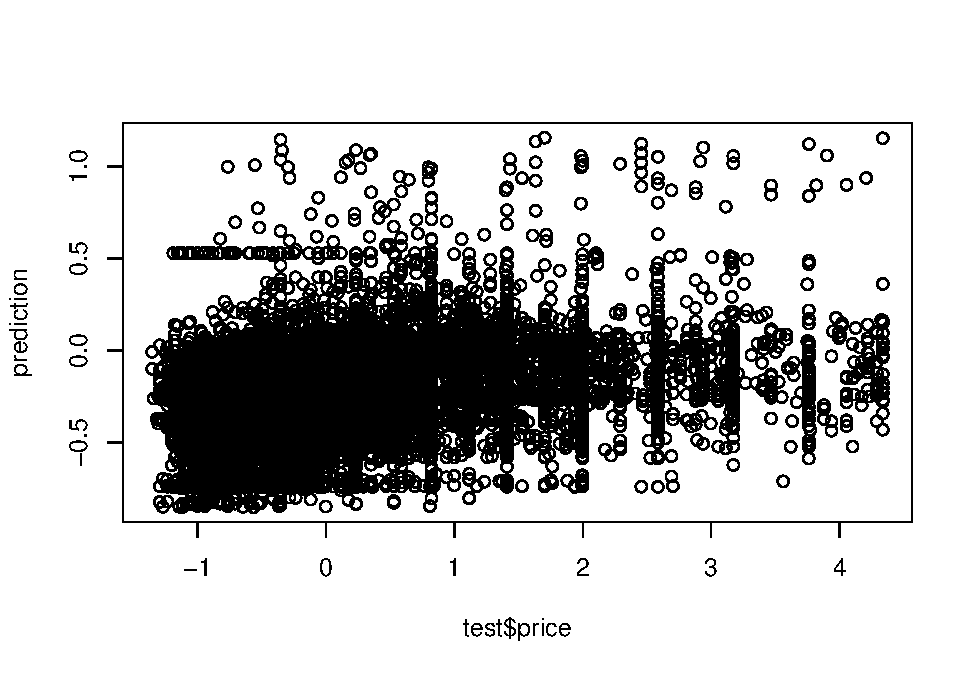
\includegraphics{project_files/figure-latex/unnamed-chunk-31-1.pdf}

\begin{Shaded}
\begin{Highlighting}[]
\KeywordTok{print}\NormalTok{(fit_rf)}
\end{Highlighting}
\end{Shaded}

\begin{verbatim}
## Random Forest 
## 
## 4717 samples
##    2 predictor
## 
## No pre-processing
## Resampling: Cross-Validated (10 fold) 
## Summary of sample sizes: 4245, 4247, 4245, 4246, 4245, 4246, ... 
## Resampling results:
## 
##   RMSE       Rsquared   MAE      
##   0.6081948  0.2609948  0.4023938
## 
## Tuning parameter 'mtry' was held constant at a value of 1
\end{verbatim}

\begin{Shaded}
\begin{Highlighting}[]
\CommentTok{#varImpPlot(fit_rf)}
\CommentTok{#plot(prediction_default, test$price)}
\end{Highlighting}
\end{Shaded}

\begin{Shaded}
\begin{Highlighting}[]
\CommentTok{## Step 6) Visualize Result}
\NormalTok{ele =}\StringTok{ }\NormalTok{randomForest}\OperatorTok{::}\KeywordTok{randomForest}\NormalTok{(}
  \DataTypeTok{x =}\NormalTok{  train_neig_room[}\OperatorTok{-}\DecValTok{3}\NormalTok{],}
  \DataTypeTok{y =}\NormalTok{ train_neig_room}\OperatorTok{$}\NormalTok{price,}
  \DataTypeTok{xtest =}\NormalTok{ test_neig_room[}\OperatorTok{-}\DecValTok{3}\NormalTok{],}
  \DataTypeTok{ytest =}\NormalTok{ test_neig_room}\OperatorTok{$}\NormalTok{price,}
  \DataTypeTok{mtry =} \DecValTok{5}\NormalTok{,}
  \DataTypeTok{maxnodes=}\DecValTok{30}\NormalTok{,}
  \DataTypeTok{ntree =} \DecValTok{800}
\NormalTok{)}
\end{Highlighting}
\end{Shaded}

\begin{verbatim}
## Warning in randomForest.default(x = train_neig_room[-3], y =
## train_neig_room$price, : invalid mtry: reset to within valid range
\end{verbatim}

\begin{Shaded}
\begin{Highlighting}[]
\KeywordTok{print}\NormalTok{(ele)}
\end{Highlighting}
\end{Shaded}

\begin{verbatim}
## 
## Call:
##  randomForest(x = train_neig_room[-3], y = train_neig_room$price,      xtest = test_neig_room[-3], ytest = test_neig_room$price,      ntree = 800, mtry = 5, maxnodes = 30) 
##                Type of random forest: regression
##                      Number of trees: 800
## No. of variables tried at each split: 2
## 
##           Mean of squared residuals: 0.3649994
##                     % Var explained: 26.99
##                        Test set MSE: 0.35
##                     % Var explained: 26.2
\end{verbatim}

\begin{Shaded}
\begin{Highlighting}[]
\KeywordTok{varImpPlot}\NormalTok{(ele)}
\end{Highlighting}
\end{Shaded}

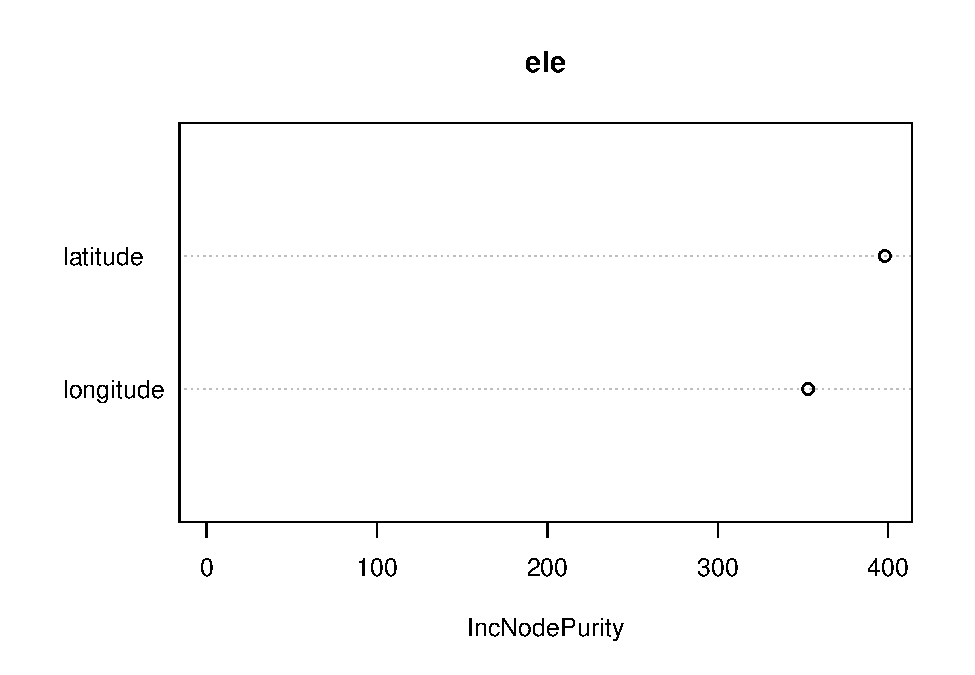
\includegraphics{project_files/figure-latex/unnamed-chunk-32-1.pdf}

\begin{Shaded}
\begin{Highlighting}[]
\KeywordTok{plot}\NormalTok{(ele)}
\end{Highlighting}
\end{Shaded}

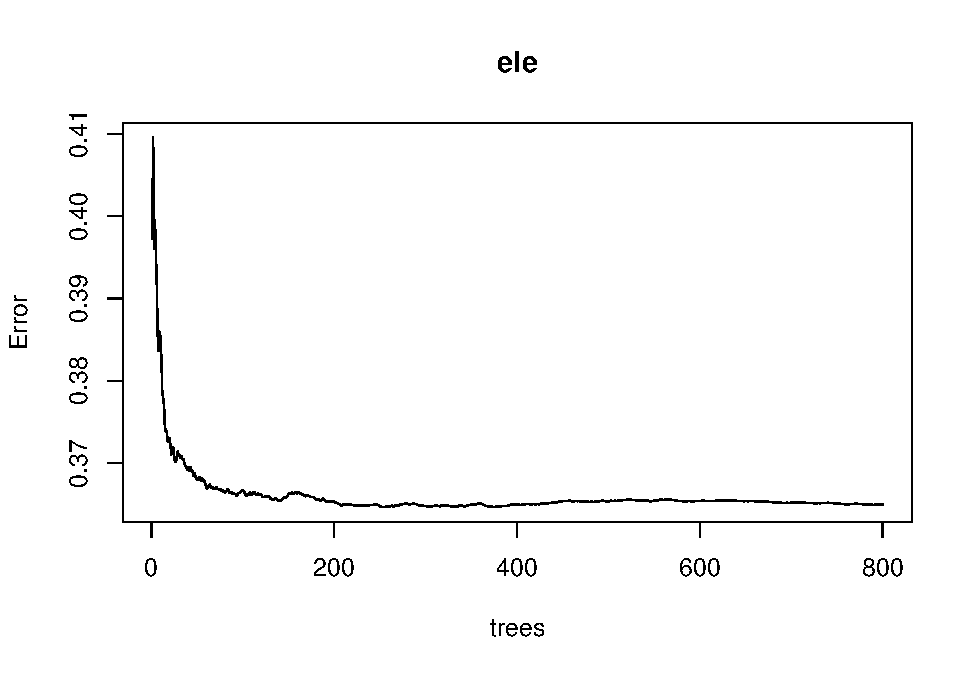
\includegraphics{project_files/figure-latex/unnamed-chunk-32-2.pdf}

\hypertarget{ranger-random-forest}{%
\section{RANGER RANDOM FOREST}\label{ranger-random-forest}}

\begin{Shaded}
\begin{Highlighting}[]
\KeywordTok{library}\NormalTok{(ranger)}
\end{Highlighting}
\end{Shaded}

\begin{verbatim}
## 
## Attaching package: 'ranger'
\end{verbatim}

\begin{verbatim}
## The following object is masked from 'package:randomForest':
## 
##     importance
\end{verbatim}

\begin{Shaded}
\begin{Highlighting}[]
\KeywordTok{library}\NormalTok{(tuneRanger)}
\end{Highlighting}
\end{Shaded}

\begin{verbatim}
## Loading required package: mlrMBO
\end{verbatim}

\begin{verbatim}
## Loading required package: mlr
\end{verbatim}

\begin{verbatim}
## Loading required package: ParamHelpers
\end{verbatim}

\begin{verbatim}
## 'mlr' is in maintenance mode since July 2019. Future development
## efforts will go into its successor 'mlr3' (<https://mlr3.mlr-org.com>).
\end{verbatim}

\begin{verbatim}
## 
## Attaching package: 'mlr'
\end{verbatim}

\begin{verbatim}
## The following object is masked _by_ '.GlobalEnv':
## 
##     mape
\end{verbatim}

\begin{verbatim}
## The following object is masked from 'package:e1071':
## 
##     impute
\end{verbatim}

\begin{verbatim}
## The following object is masked from 'package:caret':
## 
##     train
\end{verbatim}

\begin{verbatim}
## Loading required package: smoof
\end{verbatim}

\begin{verbatim}
## Loading required package: checkmate
\end{verbatim}

\begin{verbatim}
## Loading required package: lubridate
\end{verbatim}

\begin{verbatim}
## 
## Attaching package: 'lubridate'
\end{verbatim}

\begin{verbatim}
## The following objects are masked from 'package:base':
## 
##     date, intersect, setdiff, union
\end{verbatim}

\begin{verbatim}
## Loading required package: lhs
\end{verbatim}

\begin{Shaded}
\begin{Highlighting}[]
\NormalTok{rangerReg <-}\StringTok{ }\KeywordTok{ranger}\NormalTok{( price}\OperatorTok{~}\StringTok{ }\NormalTok{., }\DataTypeTok{data =}\NormalTok{ train, }\DataTypeTok{write.forest =} \OtherTok{TRUE}\NormalTok{, }\DataTypeTok{classification =}\NormalTok{ F)}
\NormalTok{rangerReg}
\end{Highlighting}
\end{Shaded}

\begin{verbatim}
## Ranger result
## 
## Call:
##  ranger(price ~ ., data = train, write.forest = TRUE, classification = F) 
## 
## Type:                             Regression 
## Number of trees:                  500 
## Sample size:                      28574 
## Number of independent variables:  4 
## Mtry:                             2 
## Target node size:                 5 
## Variable importance mode:         none 
## Splitrule:                        variance 
## OOB prediction error (MSE):       0.5391425 
## R squared (OOB):                  0.4628551
\end{verbatim}

\begin{Shaded}
\begin{Highlighting}[]
\NormalTok{rangerReg_pred =}\StringTok{ }\KeywordTok{predict}\NormalTok{(rangerReg, }\DataTypeTok{data =}\NormalTok{ test)}
\NormalTok{rangerReg_pred}
\end{Highlighting}
\end{Shaded}

\begin{verbatim}
## Ranger prediction
## 
## Type:                             Regression 
## Sample size:                      19050 
## Number of independent variables:  4
\end{verbatim}

\begin{Shaded}
\begin{Highlighting}[]
\KeywordTok{library}\NormalTok{(plotly)}
\end{Highlighting}
\end{Shaded}

\begin{verbatim}
## 
## Attaching package: 'plotly'
\end{verbatim}

\begin{verbatim}
## The following object is masked from 'package:MASS':
## 
##     select
\end{verbatim}

\begin{verbatim}
## The following object is masked from 'package:ggplot2':
## 
##     last_plot
\end{verbatim}

\begin{verbatim}
## The following object is masked from 'package:stats':
## 
##     filter
\end{verbatim}

\begin{verbatim}
## The following object is masked from 'package:graphics':
## 
##     layout
\end{verbatim}

\begin{Shaded}
\begin{Highlighting}[]
\KeywordTok{plot_ly}\NormalTok{(}\DataTypeTok{x =}\NormalTok{ test}\OperatorTok{$}\NormalTok{price, }\DataTypeTok{y =} \KeywordTok{predictions}\NormalTok{(rangerReg_pred))}
\end{Highlighting}
\end{Shaded}

\begin{verbatim}
## No trace type specified:
##   Based on info supplied, a 'scatter' trace seems appropriate.
##   Read more about this trace type -> https://plot.ly/r/reference/#scatter
\end{verbatim}

\begin{verbatim}
## No scatter mode specifed:
##   Setting the mode to markers
##   Read more about this attribute -> https://plot.ly/r/reference/#scatter-mode
\end{verbatim}

\begin{verbatim}
## Warning: `arrange_()` is deprecated as of dplyr 0.7.0.
## Please use `arrange()` instead.
## See vignette('programming') for more help
## This warning is displayed once every 8 hours.
## Call `lifecycle::last_warnings()` to see where this warning was generated.
\end{verbatim}

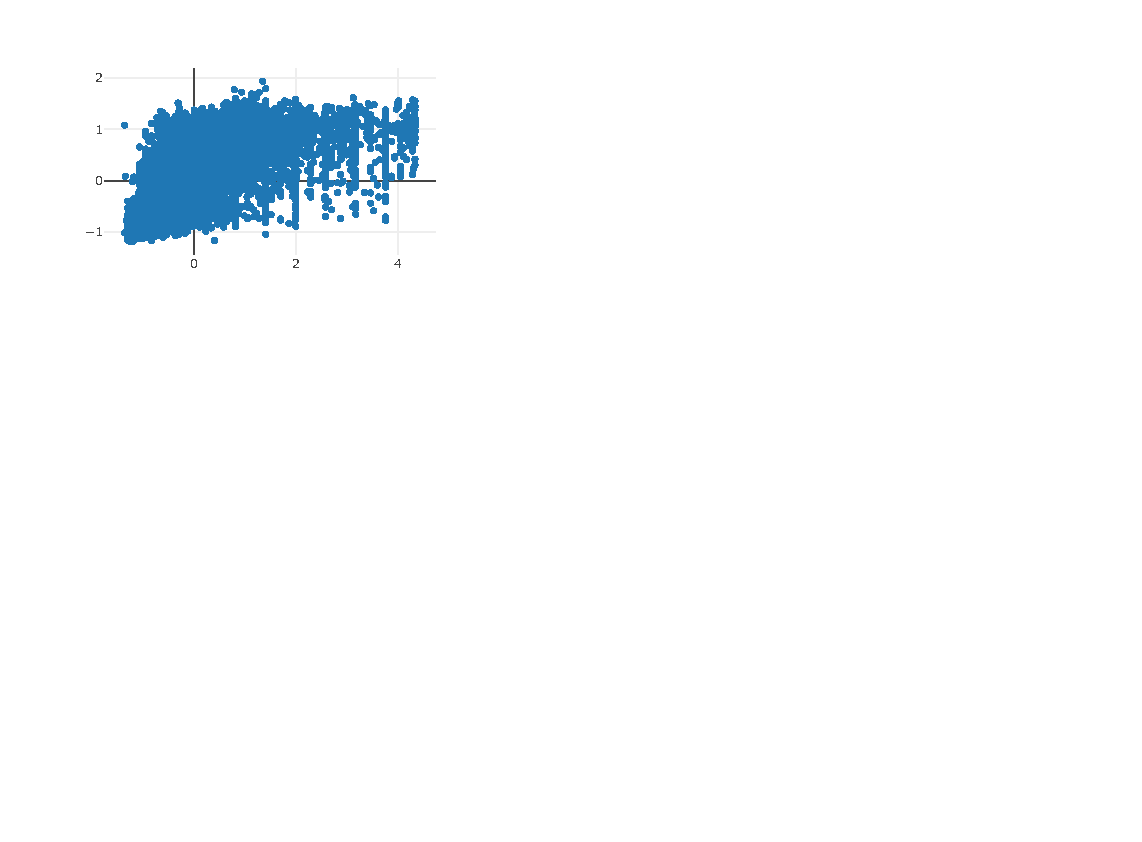
\includegraphics{project_files/figure-latex/unnamed-chunk-33-1.pdf}

\begin{Shaded}
\begin{Highlighting}[]
\KeywordTok{library}\NormalTok{(ranger)}
\KeywordTok{library}\NormalTok{(tuneRanger)}
\NormalTok{rangerReg <-}\StringTok{ }\KeywordTok{ranger}\NormalTok{( price}\OperatorTok{~}\StringTok{ }\NormalTok{., }\DataTypeTok{data =}\NormalTok{ train_neig, }\DataTypeTok{write.forest =} \OtherTok{TRUE}\NormalTok{, }\DataTypeTok{classification =}\NormalTok{ F)}
\NormalTok{rangerReg}
\end{Highlighting}
\end{Shaded}

\begin{verbatim}
## Ranger result
## 
## Call:
##  ranger(price ~ ., data = train_neig, write.forest = TRUE, classification = F) 
## 
## Type:                             Regression 
## Number of trees:                  500 
## Sample size:                      12447 
## Number of independent variables:  3 
## Mtry:                             1 
## Target node size:                 5 
## Variable importance mode:         none 
## Splitrule:                        variance 
## OOB prediction error (MSE):       0.7183535 
## R squared (OOB):                  0.3790942
\end{verbatim}

\begin{Shaded}
\begin{Highlighting}[]
\NormalTok{rangerReg_pred =}\StringTok{ }\KeywordTok{predict}\NormalTok{(rangerReg, }\DataTypeTok{data =}\NormalTok{ test_neig)}
\NormalTok{rangerReg_pred}
\end{Highlighting}
\end{Shaded}

\begin{verbatim}
## Ranger prediction
## 
## Type:                             Regression 
## Sample size:                      8298 
## Number of independent variables:  3
\end{verbatim}

\begin{Shaded}
\begin{Highlighting}[]
\KeywordTok{library}\NormalTok{(plotly)}
\KeywordTok{plot_ly}\NormalTok{(}\DataTypeTok{x =}\NormalTok{ test_neig}\OperatorTok{$}\NormalTok{price, }\DataTypeTok{y =} \KeywordTok{predictions}\NormalTok{(rangerReg_pred))}
\end{Highlighting}
\end{Shaded}

\begin{verbatim}
## No trace type specified:
##   Based on info supplied, a 'scatter' trace seems appropriate.
##   Read more about this trace type -> https://plot.ly/r/reference/#scatter
\end{verbatim}

\begin{verbatim}
## No scatter mode specifed:
##   Setting the mode to markers
##   Read more about this attribute -> https://plot.ly/r/reference/#scatter-mode
\end{verbatim}

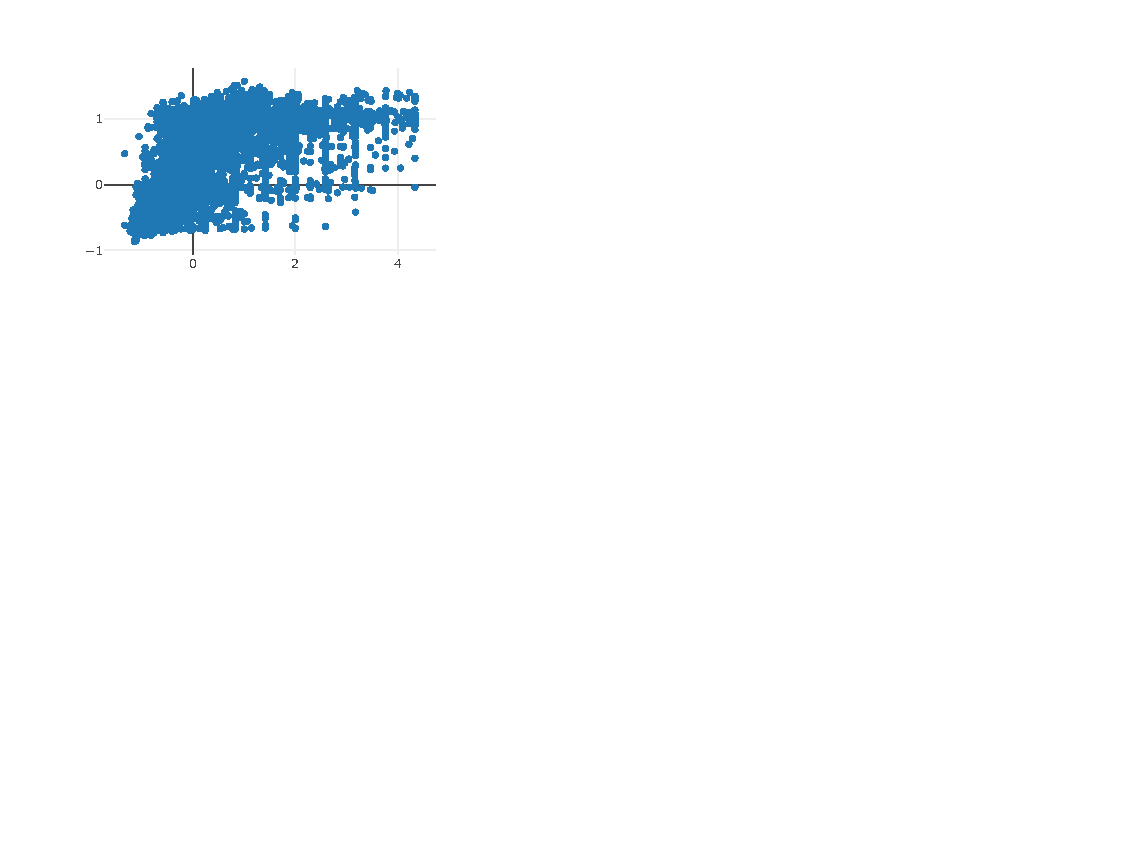
\includegraphics{project_files/figure-latex/unnamed-chunk-34-1.pdf}

\begin{Shaded}
\begin{Highlighting}[]
\NormalTok{rangerReg <-}\StringTok{ }\KeywordTok{ranger}\NormalTok{( price}\OperatorTok{~}\StringTok{ }\NormalTok{., }\DataTypeTok{data =}\NormalTok{ train_neig_room, }\DataTypeTok{write.forest =} \OtherTok{TRUE}\NormalTok{, }\DataTypeTok{classification =}\NormalTok{ F)}
\NormalTok{rangerReg}
\end{Highlighting}
\end{Shaded}

\begin{verbatim}
## Ranger result
## 
## Call:
##  ranger(price ~ ., data = train_neig_room, write.forest = TRUE,      classification = F) 
## 
## Type:                             Regression 
## Number of trees:                  500 
## Sample size:                      4717 
## Number of independent variables:  2 
## Mtry:                             1 
## Target node size:                 5 
## Variable importance mode:         none 
## Splitrule:                        variance 
## OOB prediction error (MSE):       0.3689844 
## R squared (OOB):                  0.26204
\end{verbatim}

\begin{Shaded}
\begin{Highlighting}[]
\NormalTok{rangerReg_pred =}\StringTok{ }\KeywordTok{predict}\NormalTok{(rangerReg, }\DataTypeTok{data =}\NormalTok{ test_neig_room)}
\NormalTok{rangerReg_pred}
\end{Highlighting}
\end{Shaded}

\begin{verbatim}
## Ranger prediction
## 
## Type:                             Regression 
## Sample size:                      3144 
## Number of independent variables:  2
\end{verbatim}

\begin{Shaded}
\begin{Highlighting}[]
\KeywordTok{library}\NormalTok{(plotly)}
\KeywordTok{plot_ly}\NormalTok{(}\DataTypeTok{x =}\NormalTok{ test_neig_room}\OperatorTok{$}\NormalTok{price, }\DataTypeTok{y =} \KeywordTok{predictions}\NormalTok{(rangerReg_pred))}
\end{Highlighting}
\end{Shaded}

\begin{verbatim}
## No trace type specified:
##   Based on info supplied, a 'scatter' trace seems appropriate.
##   Read more about this trace type -> https://plot.ly/r/reference/#scatter
\end{verbatim}

\begin{verbatim}
## No scatter mode specifed:
##   Setting the mode to markers
##   Read more about this attribute -> https://plot.ly/r/reference/#scatter-mode
\end{verbatim}

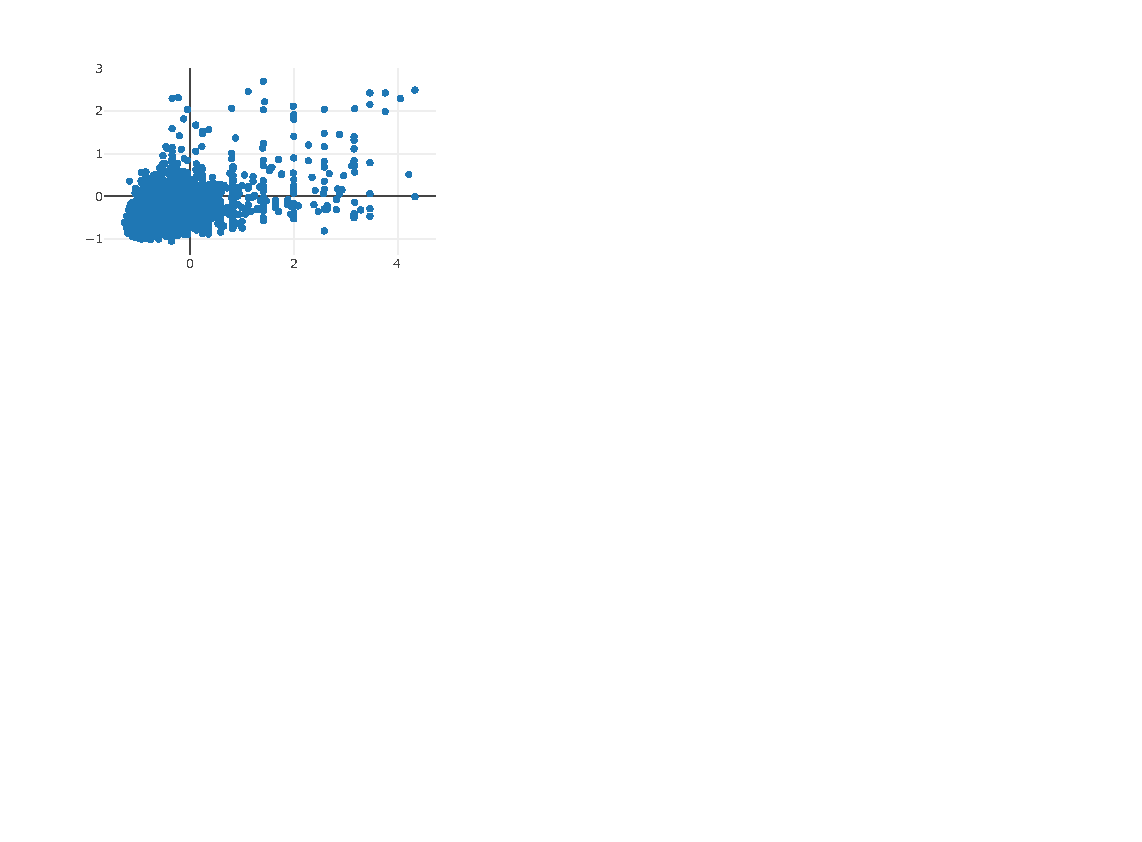
\includegraphics{project_files/figure-latex/unnamed-chunk-35-1.pdf}

\hypertarget{ranger-tuning}{%
\subsection{RANGER TUNING}\label{ranger-tuning}}

\begin{Shaded}
\begin{Highlighting}[]
\KeywordTok{library}\NormalTok{(tuneRanger)}

\CommentTok{# https://github.com/PhilippPro/tuneRanger}
\CommentTok{# https://mlr.mlr-org.com/articles/tutorial/measures.html}
\NormalTok{task =}\StringTok{ }\KeywordTok{makeRegrTask}\NormalTok{(}\DataTypeTok{data =}\NormalTok{ train, }\DataTypeTok{target =} \StringTok{"price"}\NormalTok{)}
\KeywordTok{estimateTimeTuneRanger}\NormalTok{(task, }\DataTypeTok{iters =} \DecValTok{20}\NormalTok{, }\DataTypeTok{num.threads =} \DecValTok{8}\NormalTok{, }\DataTypeTok{num.trees =} \DecValTok{1000}\NormalTok{)}
\end{Highlighting}
\end{Shaded}

\begin{verbatim}
## Approximated time for tuning: 3M 40S
\end{verbatim}

\begin{Shaded}
\begin{Highlighting}[]
\NormalTok{start.time <-}\StringTok{ }\KeywordTok{Sys.time}\NormalTok{()}

     
\NormalTok{res =}\StringTok{ }\KeywordTok{tuneRanger}\NormalTok{(task, }\DataTypeTok{measure =} \KeywordTok{list}\NormalTok{(mse), }\DataTypeTok{num.trees =} \DecValTok{1000}\NormalTok{, }
                 \DataTypeTok{num.threads =} \DecValTok{8}\NormalTok{, }\DataTypeTok{iters =} \DecValTok{20}\NormalTok{,  }\DataTypeTok{show.info =} \KeywordTok{getOption}\NormalTok{(}\StringTok{"mlrMBO.show.info"}\NormalTok{, }\OtherTok{TRUE}\NormalTok{))}
\end{Highlighting}
\end{Shaded}

\begin{verbatim}
## Computing y column(s) for design. Not provided.
\end{verbatim}

\begin{verbatim}
## [mbo] 0: mtry=4; min.node.size=224; sample.fraction=0.574 : y = 0.542 : 9.8 secs : initdesign
\end{verbatim}

\begin{verbatim}
## [mbo] 0: mtry=2; min.node.size=16; sample.fraction=0.386 : y = 0.537 : 6.3 secs : initdesign
\end{verbatim}

\begin{verbatim}
## [mbo] 0: mtry=2; min.node.size=160; sample.fraction=0.676 : y = 0.541 : 6.2 secs : initdesign
\end{verbatim}

\begin{verbatim}
## [mbo] 0: mtry=1; min.node.size=1.22e+03; sample.fraction=0.5 : y = 0.581 : 2.0 secs : initdesign
\end{verbatim}

\begin{verbatim}
## [mbo] 0: mtry=3; min.node.size=483; sample.fraction=0.797 : y = 0.545 : 7.1 secs : initdesign
\end{verbatim}

\begin{verbatim}
## [mbo] 0: mtry=3; min.node.size=7; sample.fraction=0.651 : y = 0.577 : 21.8 secs : initdesign
\end{verbatim}

\begin{verbatim}
## [mbo] 0: mtry=2; min.node.size=5; sample.fraction=0.778 : y = 0.54 : 10.2 secs : initdesign
\end{verbatim}

\begin{verbatim}
## [mbo] 0: mtry=4; min.node.size=80; sample.fraction=0.354 : y = 0.538 : 9.9 secs : initdesign
\end{verbatim}

\begin{verbatim}
## [mbo] 0: mtry=4; min.node.size=2.69e+03; sample.fraction=0.282 : y = 0.606 : 1.9 secs : initdesign
\end{verbatim}

\begin{verbatim}
## [mbo] 0: mtry=2; min.node.size=638; sample.fraction=0.43 : y = 0.552 : 3.1 secs : initdesign
\end{verbatim}

\begin{verbatim}
## [mbo] 0: mtry=1; min.node.size=3.26e+03; sample.fraction=0.548 : y = 0.603 : 1.6 secs : initdesign
\end{verbatim}

\begin{verbatim}
## [mbo] 0: mtry=1; min.node.size=6; sample.fraction=0.318 : y = 0.567 : 2.5 secs : initdesign
\end{verbatim}

\begin{verbatim}
## [mbo] 0: mtry=1; min.node.size=29; sample.fraction=0.701 : y = 0.567 : 2.7 secs : initdesign
\end{verbatim}

\begin{verbatim}
## [mbo] 0: mtry=3; min.node.size=74; sample.fraction=0.82 : y = 0.545 : 15.7 secs : initdesign
\end{verbatim}

\begin{verbatim}
## [mbo] 0: mtry=3; min.node.size=4.4e+03; sample.fraction=0.73 : y = 0.584 : 2.3 secs : initdesign
\end{verbatim}

\begin{verbatim}
## [mbo] 0: mtry=3; min.node.size=305; sample.fraction=0.245 : y = 0.547 : 3.9 secs : initdesign
\end{verbatim}

\begin{verbatim}
## [mbo] 0: mtry=4; min.node.size=32; sample.fraction=0.567 : y = 0.546 : 17.5 secs : initdesign
\end{verbatim}

\begin{verbatim}
## [mbo] 0: mtry=3; min.node.size=14; sample.fraction=0.304 : y = 0.54 : 10.2 secs : initdesign
\end{verbatim}

\begin{verbatim}
## [mbo] 0: mtry=4; min.node.size=3; sample.fraction=0.864 : y = 0.662 : 42.2 secs : initdesign
\end{verbatim}

\begin{verbatim}
## [mbo] 0: mtry=1; min.node.size=2; sample.fraction=0.636 : y = 0.567 : 2.8 secs : initdesign
\end{verbatim}

\begin{verbatim}
## [mbo] 0: mtry=2; min.node.size=382; sample.fraction=0.602 : y = 0.546 : 4.5 secs : initdesign
\end{verbatim}

\begin{verbatim}
## [mbo] 0: mtry=4; min.node.size=10; sample.fraction=0.401 : y = 0.551 : 16.9 secs : initdesign
\end{verbatim}

\begin{verbatim}
## [mbo] 0: mtry=4; min.node.size=45; sample.fraction=0.83 : y = 0.559 : 22.6 secs : initdesign
\end{verbatim}

\begin{verbatim}
## [mbo] 0: mtry=2; min.node.size=1.98e+03; sample.fraction=0.255 : y = 0.587 : 1.7 secs : initdesign
\end{verbatim}

\begin{verbatim}
## [mbo] 0: mtry=2; min.node.size=23; sample.fraction=0.477 : y = 0.537 : 6.6 secs : initdesign
\end{verbatim}

\begin{verbatim}
## [mbo] 0: mtry=1; min.node.size=102; sample.fraction=0.44 : y = 0.568 : 2.7 secs : initdesign
\end{verbatim}

\begin{verbatim}
## [mbo] 0: mtry=3; min.node.size=3; sample.fraction=0.752 : y = 0.612 : 28.5 secs : initdesign
\end{verbatim}

\begin{verbatim}
## [mbo] 0: mtry=1; min.node.size=884; sample.fraction=0.878 : y = 0.575 : 2.3 secs : initdesign
\end{verbatim}

\begin{verbatim}
## [mbo] 0: mtry=2; min.node.size=2; sample.fraction=0.218 : y = 0.537 : 5.5 secs : initdesign
\end{verbatim}

\begin{verbatim}
## [mbo] 0: mtry=4; min.node.size=1.6e+03; sample.fraction=0.524 : y = 0.564 : 3.3 secs : initdesign
\end{verbatim}

\begin{verbatim}
## [mbo] 1: mtry=2; min.node.size=5; sample.fraction=0.209 : y = 0.537 : 5.1 secs : infill_cb
\end{verbatim}

\begin{verbatim}
## [mbo] 2: mtry=2; min.node.size=19; sample.fraction=0.879 : y = 0.54 : 9.2 secs : infill_cb
\end{verbatim}

\begin{verbatim}
## [mbo] 3: mtry=3; min.node.size=77; sample.fraction=0.443 : y = 0.537 : 9.8 secs : infill_cb
\end{verbatim}

\begin{verbatim}
## [mbo] 4: mtry=4; min.node.size=20; sample.fraction=0.202 : y = 0.536 : 8.4 secs : infill_cb
\end{verbatim}

\begin{verbatim}
## [mbo] 5: mtry=2; min.node.size=7; sample.fraction=0.468 : y = 0.537 : 7.2 secs : infill_cb
\end{verbatim}

\begin{verbatim}
## [mbo] 6: mtry=3; min.node.size=37; sample.fraction=0.244 : y = 0.536 : 7.2 secs : infill_cb
\end{verbatim}

\begin{verbatim}
## [mbo] 7: mtry=2; min.node.size=44; sample.fraction=0.733 : y = 0.538 : 8.0 secs : infill_cb
\end{verbatim}

\begin{verbatim}
## [mbo] 8: mtry=4; min.node.size=32; sample.fraction=0.307 : y = 0.537 : 10.6 secs : infill_cb
\end{verbatim}

\begin{verbatim}
## [mbo] 9: mtry=3; min.node.size=25; sample.fraction=0.206 : y = 0.535 : 7.1 secs : infill_cb
\end{verbatim}

\begin{verbatim}
## [mbo] 10: mtry=2; min.node.size=12; sample.fraction=0.621 : y = 0.538 : 8.1 secs : infill_cb
\end{verbatim}

\begin{verbatim}
## [mbo] 11: mtry=2; min.node.size=4; sample.fraction=0.34 : y = 0.537 : 6.4 secs : infill_cb
\end{verbatim}

\begin{verbatim}
## [mbo] 12: mtry=3; min.node.size=60; sample.fraction=0.296 : y = 0.536 : 7.5 secs : infill_cb
\end{verbatim}

\begin{verbatim}
## [mbo] 13: mtry=2; min.node.size=8; sample.fraction=0.287 : y = 0.537 : 5.6 secs : infill_cb
\end{verbatim}

\begin{verbatim}
## [mbo] 14: mtry=3; min.node.size=22; sample.fraction=0.251 : y = 0.536 : 8.2 secs : infill_cb
\end{verbatim}

\begin{verbatim}
## [mbo] 15: mtry=4; min.node.size=56; sample.fraction=0.408 : y = 0.537 : 11.8 secs : infill_cb
\end{verbatim}

\begin{verbatim}
## [mbo] 16: mtry=3; min.node.size=38; sample.fraction=0.327 : y = 0.536 : 8.9 secs : infill_cb
\end{verbatim}

\begin{verbatim}
## [mbo] 17: mtry=3; min.node.size=30; sample.fraction=0.201 : y = 0.535 : 6.6 secs : infill_cb
\end{verbatim}

\begin{verbatim}
## [mbo] 18: mtry=2; min.node.size=64; sample.fraction=0.384 : y = 0.54 : 5.4 secs : infill_cb
\end{verbatim}

\begin{verbatim}
## [mbo] 19: mtry=2; min.node.size=97; sample.fraction=0.848 : y = 0.539 : 7.7 secs : infill_cb
\end{verbatim}

\begin{verbatim}
## [mbo] 20: mtry=4; min.node.size=24; sample.fraction=0.206 : y = 0.536 : 8.4 secs : infill_cb
\end{verbatim}

\begin{Shaded}
\begin{Highlighting}[]
\NormalTok{end.time <-}\StringTok{ }\KeywordTok{Sys.time}\NormalTok{()}
\NormalTok{time.taken <-}\StringTok{ }\NormalTok{end.time }\OperatorTok{-}\StringTok{ }\NormalTok{start.time}

\KeywordTok{print}\NormalTok{(}\StringTok{"-- Time: -- "}\NormalTok{)}
\end{Highlighting}
\end{Shaded}

\begin{verbatim}
## [1] "-- Time: -- "
\end{verbatim}

\begin{Shaded}
\begin{Highlighting}[]
\NormalTok{time.taken}
\end{Highlighting}
\end{Shaded}

\begin{verbatim}
## Time difference of 7.364678 mins
\end{verbatim}

\begin{Shaded}
\begin{Highlighting}[]
\KeywordTok{print}\NormalTok{(}\StringTok{""}\NormalTok{) }
\end{Highlighting}
\end{Shaded}

\begin{verbatim}
## [1] ""
\end{verbatim}

\begin{Shaded}
\begin{Highlighting}[]
\KeywordTok{library}\NormalTok{(tuneRanger)}

\KeywordTok{cat}\NormalTok{(}\StringTok{" === Random Forest selecting the Neighboorhood group === }\CharTok{\textbackslash{}n}\StringTok{"}\NormalTok{)}
\end{Highlighting}
\end{Shaded}

\begin{verbatim}
##  === Random Forest selecting the Neighboorhood group ===
\end{verbatim}

\begin{Shaded}
\begin{Highlighting}[]
\KeywordTok{cat}\NormalTok{(}\StringTok{"Neighboorhood group = Manhattan}\CharTok{\textbackslash{}n}\StringTok{ "}\NormalTok{)}
\end{Highlighting}
\end{Shaded}

\begin{verbatim}
## Neighboorhood group = Manhattan
## 
\end{verbatim}

\begin{Shaded}
\begin{Highlighting}[]
\NormalTok{task2 =}\StringTok{ }\KeywordTok{makeRegrTask}\NormalTok{(}\DataTypeTok{data =}\NormalTok{ train_neig, }\DataTypeTok{target =} \StringTok{"price"}\NormalTok{)}
\KeywordTok{estimateTimeTuneRanger}\NormalTok{(task2, }\DataTypeTok{iters =} \DecValTok{20}\NormalTok{, }\DataTypeTok{num.threads =} \DecValTok{8}\NormalTok{, }\DataTypeTok{num.trees =} \DecValTok{1000}\NormalTok{)}
\end{Highlighting}
\end{Shaded}

\begin{verbatim}
## Approximated time for tuning: 3M 13S
\end{verbatim}

\begin{Shaded}
\begin{Highlighting}[]
\NormalTok{start.time <-}\StringTok{ }\KeywordTok{Sys.time}\NormalTok{()}

     
\NormalTok{res2 =}\StringTok{ }\KeywordTok{tuneRanger}\NormalTok{(task2, }\DataTypeTok{measure =} \KeywordTok{list}\NormalTok{(mse), }\DataTypeTok{num.trees =} \DecValTok{1000}\NormalTok{, }
                 \DataTypeTok{num.threads =} \DecValTok{8}\NormalTok{, }\DataTypeTok{iters =} \DecValTok{20}\NormalTok{,  }\DataTypeTok{show.info =} \KeywordTok{getOption}\NormalTok{(}\StringTok{"mlrMBO.show.info"}\NormalTok{, }\OtherTok{TRUE}\NormalTok{))}
\end{Highlighting}
\end{Shaded}

\begin{verbatim}
## Computing y column(s) for design. Not provided.
\end{verbatim}

\begin{verbatim}
## [mbo] 0: mtry=1; min.node.size=216; sample.fraction=0.732 : y = 0.728 : 1.2 secs : initdesign
\end{verbatim}

\begin{verbatim}
## [mbo] 0: mtry=2; min.node.size=3; sample.fraction=0.44 : y = 0.728 : 6.0 secs : initdesign
\end{verbatim}

\begin{verbatim}
## [mbo] 0: mtry=2; min.node.size=7; sample.fraction=0.619 : y = 0.739 : 6.5 secs : initdesign
\end{verbatim}

\begin{verbatim}
## [mbo] 0: mtry=3; min.node.size=9; sample.fraction=0.349 : y = 0.708 : 5.0 secs : initdesign
\end{verbatim}

\begin{verbatim}
## [mbo] 0: mtry=1; min.node.size=49; sample.fraction=0.691 : y = 0.72 : 1.4 secs : initdesign
\end{verbatim}

\begin{verbatim}
## [mbo] 0: mtry=1; min.node.size=14; sample.fraction=0.249 : y = 0.72 : 1.1 secs : initdesign
\end{verbatim}

\begin{verbatim}
## [mbo] 0: mtry=3; min.node.size=919; sample.fraction=0.769 : y = 0.727 : 1.6 secs : initdesign
\end{verbatim}

\begin{verbatim}
## [mbo] 0: mtry=1; min.node.size=171; sample.fraction=0.52 : y = 0.728 : 1.1 secs : initdesign
\end{verbatim}

\begin{verbatim}
## [mbo] 0: mtry=2; min.node.size=89; sample.fraction=0.591 : y = 0.699 : 3.5 secs : initdesign
\end{verbatim}

\begin{verbatim}
## [mbo] 0: mtry=3; min.node.size=31; sample.fraction=0.305 : y = 0.695 : 3.5 secs : initdesign
\end{verbatim}

\begin{verbatim}
## [mbo] 0: mtry=2; min.node.size=3; sample.fraction=0.543 : y = 0.746 : 7.0 secs : initdesign
\end{verbatim}

\begin{verbatim}
## [mbo] 0: mtry=1; min.node.size=415; sample.fraction=0.633 : y = 0.732 : 1.0 secs : initdesign
\end{verbatim}

\begin{verbatim}
## [mbo] 0: mtry=2; min.node.size=377; sample.fraction=0.47 : y = 0.719 : 1.6 secs : initdesign
\end{verbatim}

\begin{verbatim}
## [mbo] 0: mtry=2; min.node.size=829; sample.fraction=0.287 : y = 0.747 : 0.9 secs : initdesign
\end{verbatim}

\begin{verbatim}
## [mbo] 0: mtry=3; min.node.size=3; sample.fraction=0.744 : y = 0.811 : 11.9 secs : initdesign
\end{verbatim}

\begin{verbatim}
## [mbo] 0: mtry=3; min.node.size=300; sample.fraction=0.572 : y = 0.715 : 2.5 secs : initdesign
\end{verbatim}

\begin{verbatim}
## [mbo] 0: mtry=3; min.node.size=2.06e+03; sample.fraction=0.407 : y = 0.779 : 0.8 secs : initdesign
\end{verbatim}

\begin{verbatim}
## [mbo] 0: mtry=1; min.node.size=5; sample.fraction=0.422 : y = 0.719 : 1.3 secs : initdesign
\end{verbatim}

\begin{verbatim}
## [mbo] 0: mtry=2; min.node.size=55; sample.fraction=0.329 : y = 0.696 : 2.6 secs : initdesign
\end{verbatim}

\begin{verbatim}
## [mbo] 0: mtry=1; min.node.size=13; sample.fraction=0.675 : y = 0.717 : 1.4 secs : initdesign
\end{verbatim}

\begin{verbatim}
## [mbo] 0: mtry=1; min.node.size=1.2e+03; sample.fraction=0.865 : y = 0.742 : 0.9 secs : initdesign
\end{verbatim}

\begin{verbatim}
## [mbo] 0: mtry=2; min.node.size=83; sample.fraction=0.814 : y = 0.704 : 4.2 secs : initdesign
\end{verbatim}

\begin{verbatim}
## [mbo] 0: mtry=2; min.node.size=2; sample.fraction=0.798 : y = 0.808 : 10.4 secs : initdesign
\end{verbatim}

\begin{verbatim}
## [mbo] 0: mtry=3; min.node.size=7; sample.fraction=0.503 : y = 0.733 : 7.3 secs : initdesign
\end{verbatim}

\begin{verbatim}
## [mbo] 0: mtry=3; min.node.size=1.5e+03; sample.fraction=0.658 : y = 0.745 : 1.2 secs : initdesign
\end{verbatim}

\begin{verbatim}
## [mbo] 0: mtry=3; min.node.size=111; sample.fraction=0.227 : y = 0.71 : 2.1 secs : initdesign
\end{verbatim}

\begin{verbatim}
## [mbo] 0: mtry=1; min.node.size=23; sample.fraction=0.883 : y = 0.718 : 1.4 secs : initdesign
\end{verbatim}

\begin{verbatim}
## [mbo] 0: mtry=2; min.node.size=2; sample.fraction=0.201 : y = 0.699 : 3.7 secs : initdesign
\end{verbatim}

\begin{verbatim}
## [mbo] 0: mtry=3; min.node.size=26; sample.fraction=0.853 : y = 0.747 : 8.5 secs : initdesign
\end{verbatim}

\begin{verbatim}
## [mbo] 0: mtry=1; min.node.size=629; sample.fraction=0.374 : y = 0.745 : 0.9 secs : initdesign
\end{verbatim}

\begin{verbatim}
## [mbo] 1: mtry=2; min.node.size=27; sample.fraction=0.414 : y = 0.696 : 3.5 secs : infill_cb
\end{verbatim}

\begin{verbatim}
## [mbo] 2: mtry=3; min.node.size=53; sample.fraction=0.406 : y = 0.697 : 3.8 secs : infill_cb
\end{verbatim}

\begin{verbatim}
## [mbo] 3: mtry=3; min.node.size=33; sample.fraction=0.204 : y = 0.696 : 2.7 secs : infill_cb
\end{verbatim}

\begin{verbatim}
## [mbo] 4: mtry=2; min.node.size=20; sample.fraction=0.278 : y = 0.693 : 2.9 secs : infill_cb
\end{verbatim}

\begin{verbatim}
## [mbo] 5: mtry=2; min.node.size=11; sample.fraction=0.2 : y = 0.694 : 2.7 secs : infill_cb
\end{verbatim}

\begin{verbatim}
## [mbo] 6: mtry=2; min.node.size=18; sample.fraction=0.2 : y = 0.693 : 2.5 secs : infill_cb
\end{verbatim}

\begin{verbatim}
## [mbo] 7: mtry=2; min.node.size=26; sample.fraction=0.251 : y = 0.694 : 2.6 secs : infill_cb
\end{verbatim}

\begin{verbatim}
## [mbo] 8: mtry=2; min.node.size=15; sample.fraction=0.232 : y = 0.694 : 2.7 secs : infill_cb
\end{verbatim}

\begin{verbatim}
## [mbo] 9: mtry=2; min.node.size=21; sample.fraction=0.324 : y = 0.694 : 3.2 secs : infill_cb
\end{verbatim}

\begin{verbatim}
## [mbo] 10: mtry=2; min.node.size=27; sample.fraction=0.287 : y = 0.693 : 2.8 secs : infill_cb
\end{verbatim}

\begin{verbatim}
## [mbo] 11: mtry=2; min.node.size=34; sample.fraction=0.288 : y = 0.695 : 2.6 secs : infill_cb
\end{verbatim}

\begin{verbatim}
## [mbo] 12: mtry=2; min.node.size=8; sample.fraction=0.205 : y = 0.694 : 2.9 secs : infill_cb
\end{verbatim}

\begin{verbatim}
## [mbo] 13: mtry=2; min.node.size=25; sample.fraction=0.302 : y = 0.693 : 3.0 secs : infill_cb
\end{verbatim}

\begin{verbatim}
## [mbo] 14: mtry=2; min.node.size=23; sample.fraction=0.287 : y = 0.694 : 2.9 secs : infill_cb
\end{verbatim}

\begin{verbatim}
## [mbo] 15: mtry=2; min.node.size=18; sample.fraction=0.268 : y = 0.694 : 2.9 secs : infill_cb
\end{verbatim}

\begin{verbatim}
## [mbo] 16: mtry=2; min.node.size=14; sample.fraction=0.206 : y = 0.693 : 2.6 secs : infill_cb
\end{verbatim}

\begin{verbatim}
## [mbo] 17: mtry=2; min.node.size=20; sample.fraction=0.208 : y = 0.693 : 2.4 secs : infill_cb
\end{verbatim}

\begin{verbatim}
## [mbo] 18: mtry=2; min.node.size=15; sample.fraction=0.203 : y = 0.693 : 2.6 secs : infill_cb
\end{verbatim}

\begin{verbatim}
## [mbo] 19: mtry=2; min.node.size=27; sample.fraction=0.313 : y = 0.694 : 3.0 secs : infill_cb
\end{verbatim}

\begin{verbatim}
## [mbo] 20: mtry=2; min.node.size=26; sample.fraction=0.283 : y = 0.693 : 2.8 secs : infill_cb
\end{verbatim}

\begin{Shaded}
\begin{Highlighting}[]
\NormalTok{end.time <-}\StringTok{ }\KeywordTok{Sys.time}\NormalTok{()}
\NormalTok{time.taken <-}\StringTok{ }\NormalTok{end.time }\OperatorTok{-}\StringTok{ }\NormalTok{start.time}

\KeywordTok{print}\NormalTok{(}\StringTok{"-- Time: -- "}\NormalTok{)}
\end{Highlighting}
\end{Shaded}

\begin{verbatim}
## [1] "-- Time: -- "
\end{verbatim}

\begin{Shaded}
\begin{Highlighting}[]
\NormalTok{time.taken}
\end{Highlighting}
\end{Shaded}

\begin{verbatim}
## Time difference of 2.755139 mins
\end{verbatim}

\begin{Shaded}
\begin{Highlighting}[]
\KeywordTok{print}\NormalTok{(}\StringTok{""}\NormalTok{)}
\end{Highlighting}
\end{Shaded}

\begin{verbatim}
## [1] ""
\end{verbatim}

\begin{Shaded}
\begin{Highlighting}[]
\KeywordTok{library}\NormalTok{(tuneRanger)}

\KeywordTok{cat}\NormalTok{(}\StringTok{" === Ranger Random Forest selecting the Neighboorhood group and room_type=== }\CharTok{\textbackslash{}n}\StringTok{"}\NormalTok{)}
\end{Highlighting}
\end{Shaded}

\begin{verbatim}
##  === Ranger Random Forest selecting the Neighboorhood group and room_type===
\end{verbatim}

\begin{Shaded}
\begin{Highlighting}[]
\KeywordTok{cat}\NormalTok{(}\StringTok{"Neighboorhood group = Manhattan and room_type=Entire-home/Apt}\CharTok{\textbackslash{}n}\StringTok{ "}\NormalTok{)}
\end{Highlighting}
\end{Shaded}

\begin{verbatim}
## Neighboorhood group = Manhattan and room_type=Entire-home/Apt
## 
\end{verbatim}

\begin{Shaded}
\begin{Highlighting}[]
\NormalTok{task3 =}\StringTok{ }\KeywordTok{makeRegrTask}\NormalTok{(}\DataTypeTok{data =}\NormalTok{ train_neig_room, }\DataTypeTok{target =} \StringTok{"price"}\NormalTok{)}
\KeywordTok{estimateTimeTuneRanger}\NormalTok{(task3, }\DataTypeTok{iters =} \DecValTok{20}\NormalTok{, }\DataTypeTok{num.threads =} \DecValTok{8}\NormalTok{, }\DataTypeTok{num.trees =} \DecValTok{1000}\NormalTok{)}
\end{Highlighting}
\end{Shaded}

\begin{verbatim}
## Approximated time for tuning: 1M 24S
\end{verbatim}

\begin{Shaded}
\begin{Highlighting}[]
\NormalTok{start.time <-}\StringTok{ }\KeywordTok{Sys.time}\NormalTok{()}

     
\NormalTok{res3 =}\StringTok{ }\KeywordTok{tuneRanger}\NormalTok{(task3, }\DataTypeTok{measure =} \KeywordTok{list}\NormalTok{(mse), }\DataTypeTok{num.trees =} \DecValTok{1000}\NormalTok{, }
                 \DataTypeTok{num.threads =} \DecValTok{8}\NormalTok{, }\DataTypeTok{iters =} \DecValTok{20}\NormalTok{,  }\DataTypeTok{show.info =} \KeywordTok{getOption}\NormalTok{(}\StringTok{"mlrMBO.show.info"}\NormalTok{, }\OtherTok{TRUE}\NormalTok{))}
\end{Highlighting}
\end{Shaded}

\begin{verbatim}
## Computing y column(s) for design. Not provided.
\end{verbatim}

\begin{verbatim}
## [mbo] 0: mtry=2; min.node.size=26; sample.fraction=0.799 : y = 0.365 : 2.3 secs : initdesign
\end{verbatim}

\begin{verbatim}
## [mbo] 0: mtry=2; min.node.size=3; sample.fraction=0.605 : y = 0.38 : 3.1 secs : initdesign
\end{verbatim}

\begin{verbatim}
## [mbo] 0: mtry=2; min.node.size=13; sample.fraction=0.487 : y = 0.357 : 1.9 secs : initdesign
\end{verbatim}

\begin{verbatim}
## [mbo] 0: mtry=1; min.node.size=85; sample.fraction=0.463 : y = 0.368 : 0.8 secs : initdesign
\end{verbatim}

\begin{verbatim}
## [mbo] 0: mtry=1; min.node.size=203; sample.fraction=0.682 : y = 0.378 : 0.7 secs : initdesign
\end{verbatim}

\begin{verbatim}
## [mbo] 0: mtry=1; min.node.size=7; sample.fraction=0.832 : y = 0.379 : 2.2 secs : initdesign
\end{verbatim}

\begin{verbatim}
## [mbo] 0: mtry=2; min.node.size=376; sample.fraction=0.663 : y = 0.386 : 0.7 secs : initdesign
\end{verbatim}

\begin{verbatim}
## [mbo] 0: mtry=1; min.node.size=14; sample.fraction=0.411 : y = 0.352 : 1.1 secs : initdesign
\end{verbatim}

\begin{verbatim}
## [mbo] 0: mtry=2; min.node.size=45; sample.fraction=0.626 : y = 0.355 : 1.6 secs : initdesign
\end{verbatim}

\begin{verbatim}
## [mbo] 0: mtry=1; min.node.size=258; sample.fraction=0.252 : y = 0.397 : 0.4 secs : initdesign
\end{verbatim}

\begin{verbatim}
## [mbo] 0: mtry=2; min.node.size=9; sample.fraction=0.303 : y = 0.353 : 1.5 secs : initdesign
\end{verbatim}

\begin{verbatim}
## [mbo] 0: mtry=2; min.node.size=662; sample.fraction=0.386 : y = 0.409 : 0.4 secs : initdesign
\end{verbatim}

\begin{verbatim}
## [mbo] 0: mtry=1; min.node.size=2; sample.fraction=0.327 : y = 0.355 : 1.5 secs : initdesign
\end{verbatim}

\begin{verbatim}
## [mbo] 0: mtry=1; min.node.size=21; sample.fraction=0.733 : y = 0.357 : 1.5 secs : initdesign
\end{verbatim}

\begin{verbatim}
## [mbo] 0: mtry=1; min.node.size=2; sample.fraction=0.819 : y = 0.396 : 3.0 secs : initdesign
\end{verbatim}

\begin{verbatim}
## [mbo] 0: mtry=2; min.node.size=110; sample.fraction=0.753 : y = 0.366 : 1.2 secs : initdesign
\end{verbatim}

\begin{verbatim}
## [mbo] 0: mtry=2; min.node.size=154; sample.fraction=0.433 : y = 0.377 : 0.8 secs : initdesign
\end{verbatim}

\begin{verbatim}
## [mbo] 0: mtry=2; min.node.size=6; sample.fraction=0.531 : y = 0.366 : 2.4 secs : initdesign
\end{verbatim}

\begin{verbatim}
## [mbo] 0: mtry=1; min.node.size=19; sample.fraction=0.241 : y = 0.356 : 0.8 secs : initdesign
\end{verbatim}

\begin{verbatim}
## [mbo] 0: mtry=1; min.node.size=32; sample.fraction=0.55 : y = 0.353 : 1.1 secs : initdesign
\end{verbatim}

\begin{verbatim}
## [mbo] 0: mtry=1; min.node.size=396; sample.fraction=0.574 : y = 0.388 : 0.5 secs : initdesign
\end{verbatim}

\begin{verbatim}
## [mbo] 0: mtry=1; min.node.size=75; sample.fraction=0.206 : y = 0.377 : 0.6 secs : initdesign
\end{verbatim}

\begin{verbatim}
## [mbo] 0: mtry=2; min.node.size=3; sample.fraction=0.77 : y = 0.404 : 3.8 secs : initdesign
\end{verbatim}

\begin{verbatim}
## [mbo] 0: mtry=2; min.node.size=51; sample.fraction=0.39 : y = 0.358 : 1.1 secs : initdesign
\end{verbatim}

\begin{verbatim}
## [mbo] 0: mtry=2; min.node.size=596; sample.fraction=0.882 : y = 0.393 : 0.6 secs : initdesign
\end{verbatim}

\begin{verbatim}
## [mbo] 0: mtry=2; min.node.size=5; sample.fraction=0.695 : y = 0.384 : 3.1 secs : initdesign
\end{verbatim}

\begin{verbatim}
## [mbo] 0: mtry=1; min.node.size=4; sample.fraction=0.522 : y = 0.364 : 1.7 secs : initdesign
\end{verbatim}

\begin{verbatim}
## [mbo] 0: mtry=1; min.node.size=887; sample.fraction=0.353 : y = 0.422 : 0.4 secs : initdesign
\end{verbatim}

\begin{verbatim}
## [mbo] 0: mtry=2; min.node.size=2; sample.fraction=0.283 : y = 0.356 : 1.9 secs : initdesign
\end{verbatim}

\begin{verbatim}
## [mbo] 0: mtry=1; min.node.size=148; sample.fraction=0.871 : y = 0.369 : 0.8 secs : initdesign
\end{verbatim}

\begin{verbatim}
## [mbo] 1: mtry=2; min.node.size=13; sample.fraction=0.226 : y = 0.353 : 1.2 secs : infill_cb
\end{verbatim}

\begin{verbatim}
## [mbo] 2: mtry=1; min.node.size=3; sample.fraction=0.2 : y = 0.352 : 1.0 secs : infill_cb
\end{verbatim}

\begin{verbatim}
## [mbo] 3: mtry=1; min.node.size=7; sample.fraction=0.265 : y = 0.352 : 1.0 secs : infill_cb
\end{verbatim}

\begin{verbatim}
## [mbo] 4: mtry=1; min.node.size=2; sample.fraction=0.203 : y = 0.352 : 1.1 secs : infill_cb
\end{verbatim}

\begin{verbatim}
## [mbo] 5: mtry=2; min.node.size=4; sample.fraction=0.203 : y = 0.352 : 1.3 secs : infill_cb
\end{verbatim}

\begin{verbatim}
## [mbo] 6: mtry=1; min.node.size=22; sample.fraction=0.574 : y = 0.353 : 1.2 secs : infill_cb
\end{verbatim}

\begin{verbatim}
## [mbo] 7: mtry=1; min.node.size=5; sample.fraction=0.21 : y = 0.352 : 1.0 secs : infill_cb
\end{verbatim}

\begin{verbatim}
## [mbo] 8: mtry=2; min.node.size=19; sample.fraction=0.343 : y = 0.351 : 1.4 secs : infill_cb
\end{verbatim}

\begin{verbatim}
## [mbo] 9: mtry=2; min.node.size=16; sample.fraction=0.298 : y = 0.351 : 1.3 secs : infill_cb
\end{verbatim}

\begin{verbatim}
## [mbo] 10: mtry=1; min.node.size=12; sample.fraction=0.32 : y = 0.352 : 1.1 secs : infill_cb
\end{verbatim}

\begin{verbatim}
## [mbo] 11: mtry=2; min.node.size=15; sample.fraction=0.342 : y = 0.351 : 1.6 secs : infill_cb
\end{verbatim}

\begin{verbatim}
## [mbo] 12: mtry=2; min.node.size=15; sample.fraction=0.327 : y = 0.351 : 1.5 secs : infill_cb
\end{verbatim}

\begin{verbatim}
## [mbo] 13: mtry=2; min.node.size=17; sample.fraction=0.367 : y = 0.352 : 1.5 secs : infill_cb
\end{verbatim}

\begin{verbatim}
## [mbo] 14: mtry=2; min.node.size=15; sample.fraction=0.315 : y = 0.351 : 1.5 secs : infill_cb
\end{verbatim}

\begin{verbatim}
## [mbo] 15: mtry=2; min.node.size=17; sample.fraction=0.335 : y = 0.352 : 1.4 secs : infill_cb
\end{verbatim}

\begin{verbatim}
## [mbo] 16: mtry=2; min.node.size=15; sample.fraction=0.308 : y = 0.352 : 1.4 secs : infill_cb
\end{verbatim}

\begin{verbatim}
## [mbo] 17: mtry=2; min.node.size=16; sample.fraction=0.339 : y = 0.351 : 1.5 secs : infill_cb
\end{verbatim}

\begin{verbatim}
## [mbo] 18: mtry=2; min.node.size=15; sample.fraction=0.327 : y = 0.351 : 1.4 secs : infill_cb
\end{verbatim}

\begin{verbatim}
## [mbo] 19: mtry=2; min.node.size=14; sample.fraction=0.324 : y = 0.352 : 1.4 secs : infill_cb
\end{verbatim}

\begin{verbatim}
## [mbo] 20: mtry=2; min.node.size=16; sample.fraction=0.328 : y = 0.351 : 1.4 secs : infill_cb
\end{verbatim}

\begin{Shaded}
\begin{Highlighting}[]
\NormalTok{end.time <-}\StringTok{ }\KeywordTok{Sys.time}\NormalTok{()}
\NormalTok{time.taken <-}\StringTok{ }\NormalTok{end.time }\OperatorTok{-}\StringTok{ }\NormalTok{start.time}

\KeywordTok{print}\NormalTok{(}\StringTok{"-- Time: -- "}\NormalTok{)}
\end{Highlighting}
\end{Shaded}

\begin{verbatim}
## [1] "-- Time: -- "
\end{verbatim}

\begin{Shaded}
\begin{Highlighting}[]
\NormalTok{time.taken}
\end{Highlighting}
\end{Shaded}

\begin{verbatim}
## Time difference of 1.256275 mins
\end{verbatim}

\begin{Shaded}
\begin{Highlighting}[]
\KeywordTok{print}\NormalTok{(}\StringTok{""}\NormalTok{)  }
\end{Highlighting}
\end{Shaded}

\begin{verbatim}
## [1] ""
\end{verbatim}

Mean of best 5 \% of the results

\begin{Shaded}
\begin{Highlighting}[]
\NormalTok{res}\OperatorTok{$}\NormalTok{model}
\end{Highlighting}
\end{Shaded}

\begin{verbatim}
## Model for learner.id=regr.ranger; learner.class=regr.ranger
## Trained on: task.id = train; obs = 28574; features = 4
## Hyperparameters: num.threads=8,verbose=FALSE,respect.unordered.factors=order,mtry=3,min.node.size=26,sample.fraction=0.204,num.trees=1e+03,replace=FALSE
\end{verbatim}

Recommended parameter settings: mtry min.node.size sample.fraction 1 2
55 0.2136541 Results: mse exec.time 1 0.933998 2.756667

Model with the new tuned hyperparameters

\begin{Shaded}
\begin{Highlighting}[]
\NormalTok{res2}\OperatorTok{$}\NormalTok{model}
\end{Highlighting}
\end{Shaded}

\begin{verbatim}
## Model for learner.id=regr.ranger; learner.class=regr.ranger
## Trained on: task.id = train_neig; obs = 12447; features = 3
## Hyperparameters: num.threads=8,verbose=FALSE,respect.unordered.factors=order,mtry=2,min.node.size=16,sample.fraction=0.206,num.trees=1e+03,replace=FALSE
\end{verbatim}

Model with the new tuned hyperparameters

\begin{Shaded}
\begin{Highlighting}[]
\NormalTok{res3}\OperatorTok{$}\NormalTok{model}
\end{Highlighting}
\end{Shaded}

\begin{verbatim}
## Model for learner.id=regr.ranger; learner.class=regr.ranger
## Trained on: task.id = train_neig_room; obs = 4717; features = 2
## Hyperparameters: num.threads=8,verbose=FALSE,respect.unordered.factors=order,mtry=2,min.node.size=15,sample.fraction=0.333,num.trees=1e+03,replace=FALSE
\end{verbatim}

\begin{Shaded}
\begin{Highlighting}[]
\NormalTok{tuned_rangerReg <-}\StringTok{ }\KeywordTok{ranger}\NormalTok{( price}\OperatorTok{~}\StringTok{ }\NormalTok{., }\DataTypeTok{data =}\NormalTok{ train, }\DataTypeTok{write.forest =} \OtherTok{TRUE}\NormalTok{, }\DataTypeTok{classification =}\NormalTok{ F, }\DataTypeTok{mtry=} \DecValTok{3}\NormalTok{, }
                           \DataTypeTok{min.node.size =} \DecValTok{35}\NormalTok{   , }\DataTypeTok{sample.fraction =} \FloatTok{0.326}\NormalTok{,}\DataTypeTok{num.trees =} \DecValTok{1000}\NormalTok{, }\DataTypeTok{replace=} \OtherTok{FALSE}\NormalTok{)}
\NormalTok{tuned_rangerReg}
\end{Highlighting}
\end{Shaded}

\begin{verbatim}
## Ranger result
## 
## Call:
##  ranger(price ~ ., data = train, write.forest = TRUE, classification = F,      mtry = 3, min.node.size = 35, sample.fraction = 0.326, num.trees = 1000,      replace = FALSE) 
## 
## Type:                             Regression 
## Number of trees:                  1000 
## Sample size:                      28574 
## Number of independent variables:  4 
## Mtry:                             3 
## Target node size:                 35 
## Variable importance mode:         none 
## Splitrule:                        variance 
## OOB prediction error (MSE):       0.5359859 
## R squared (OOB):                  0.466
\end{verbatim}

\begin{Shaded}
\begin{Highlighting}[]
\NormalTok{tuned_rangerReg_pred =}\StringTok{ }\KeywordTok{predict}\NormalTok{(tuned_rangerReg, }\DataTypeTok{data =}\NormalTok{ test)}
\NormalTok{tuned_rangerReg_pred}
\end{Highlighting}
\end{Shaded}

\begin{verbatim}
## Ranger prediction
## 
## Type:                             Regression 
## Sample size:                      19050 
## Number of independent variables:  4
\end{verbatim}

\begin{Shaded}
\begin{Highlighting}[]
\CommentTok{#Hyperparameters: num.threads=8,verbose=FALSE,respect.unordered.factors=order,}
\CommentTok{#mtry=2,min.node.size=22,sample.fraction=0.231,num.trees=1e+03,replace=FALSE}

\NormalTok{tuned_rangerReg2 <-}\StringTok{ }\KeywordTok{ranger}\NormalTok{( price}\OperatorTok{~}\StringTok{ }\NormalTok{., }\DataTypeTok{data =}\NormalTok{ train_neig, }\DataTypeTok{write.forest =} \OtherTok{TRUE}\NormalTok{, }\DataTypeTok{classification =}\NormalTok{ F, }\DataTypeTok{mtry=} \DecValTok{2}\NormalTok{, }
                           \DataTypeTok{min.node.size =} \DecValTok{22}\NormalTok{, }\DataTypeTok{sample.fraction =} \FloatTok{0.231}\NormalTok{,}\DataTypeTok{num.trees =} \DecValTok{1000}\NormalTok{, }\DataTypeTok{replace=} \OtherTok{FALSE}\NormalTok{)}
\NormalTok{tuned_rangerReg2}
\end{Highlighting}
\end{Shaded}

\begin{verbatim}
## Ranger result
## 
## Call:
##  ranger(price ~ ., data = train_neig, write.forest = TRUE, classification = F,      mtry = 2, min.node.size = 22, sample.fraction = 0.231, num.trees = 1000,      replace = FALSE) 
## 
## Type:                             Regression 
## Number of trees:                  1000 
## Sample size:                      12447 
## Number of independent variables:  3 
## Mtry:                             2 
## Target node size:                 22 
## Variable importance mode:         none 
## Splitrule:                        variance 
## OOB prediction error (MSE):       0.6927535 
## R squared (OOB):                  0.4012214
\end{verbatim}

\begin{Shaded}
\begin{Highlighting}[]
\NormalTok{tuned_rangerReg_pred2 =}\StringTok{ }\KeywordTok{predict}\NormalTok{(tuned_rangerReg2, }\DataTypeTok{data =}\NormalTok{ test_neig)}
\NormalTok{tuned_rangerReg_pred2}
\end{Highlighting}
\end{Shaded}

\begin{verbatim}
## Ranger prediction
## 
## Type:                             Regression 
## Sample size:                      8298 
## Number of independent variables:  3
\end{verbatim}

\begin{Shaded}
\begin{Highlighting}[]
\CommentTok{#Hyperparameters: num.threads=8,verbose=FALSE,respect.unordered.factors=order,mtry=1,min.node.size=5,sample.fraction=0.21,num.trees=1e+03,replace=FALSE}

\NormalTok{tuned_rangerReg3 <-}\StringTok{ }\KeywordTok{ranger}\NormalTok{( price}\OperatorTok{~}\StringTok{ }\NormalTok{., }\DataTypeTok{data =}\NormalTok{ train_neig_room, }\DataTypeTok{write.forest =} \OtherTok{TRUE}\NormalTok{, }\DataTypeTok{classification =}\NormalTok{ F, }\DataTypeTok{mtry=}\DecValTok{1}\NormalTok{, }
                           \DataTypeTok{min.node.size =} \DecValTok{5}\NormalTok{    , }\DataTypeTok{sample.fraction =} \FloatTok{0.21}\NormalTok{,}\DataTypeTok{num.trees =} \DecValTok{1000}\NormalTok{, }\DataTypeTok{replace=} \OtherTok{FALSE}\NormalTok{)}
\NormalTok{tuned_rangerReg3}
\end{Highlighting}
\end{Shaded}

\begin{verbatim}
## Ranger result
## 
## Call:
##  ranger(price ~ ., data = train_neig_room, write.forest = TRUE,      classification = F, mtry = 1, min.node.size = 5, sample.fraction = 0.21,      num.trees = 1000, replace = FALSE) 
## 
## Type:                             Regression 
## Number of trees:                  1000 
## Sample size:                      4717 
## Number of independent variables:  2 
## Mtry:                             1 
## Target node size:                 5 
## Variable importance mode:         none 
## Splitrule:                        variance 
## OOB prediction error (MSE):       0.3518077 
## R squared (OOB):                  0.2963931
\end{verbatim}

\begin{Shaded}
\begin{Highlighting}[]
\NormalTok{tuned_rangerReg_pred3 =}\StringTok{ }\KeywordTok{predict}\NormalTok{(tuned_rangerReg3, }\DataTypeTok{data =}\NormalTok{ test_neig_room)}
\NormalTok{tuned_rangerReg_pred3}
\end{Highlighting}
\end{Shaded}

\begin{verbatim}
## Ranger prediction
## 
## Type:                             Regression 
## Sample size:                      3144 
## Number of independent variables:  2
\end{verbatim}

\hypertarget{neural-networks}{%
\section{NEURAL NETWORKS}\label{neural-networks}}

\url{https://medium.com/@brscntyz/neural-network-in-r-e275302b6e44}
\url{https://datascienceplus.com/fitting-neural-network-in-r/}
\url{https://www.kdnuggets.com/2016/08/begineers-guide-neural-networks-r.html/2}

\begin{Shaded}
\begin{Highlighting}[]
\KeywordTok{library}\NormalTok{(ISLR)}
\KeywordTok{library}\NormalTok{(tidyverse)}
\KeywordTok{library}\NormalTok{(}\StringTok{"keras"}\NormalTok{)}
\end{Highlighting}
\end{Shaded}

\begin{verbatim}
## 
## Attaching package: 'keras'
\end{verbatim}

\begin{verbatim}
## The following object is masked _by_ '.GlobalEnv':
## 
##     normalize
\end{verbatim}

\begin{verbatim}
## The following object is masked from 'package:future':
## 
##     %<-%
\end{verbatim}

\begin{Shaded}
\begin{Highlighting}[]
\KeywordTok{library}\NormalTok{(neuralnet)}
\end{Highlighting}
\end{Shaded}

\begin{verbatim}
## 
## Attaching package: 'neuralnet'
\end{verbatim}

\begin{verbatim}
## The following object is masked from 'package:dplyr':
## 
##     compute
\end{verbatim}

\begin{Shaded}
\begin{Highlighting}[]
\KeywordTok{library}\NormalTok{(Hmisc)}
\end{Highlighting}
\end{Shaded}

\begin{verbatim}
## Loading required package: survival
\end{verbatim}

\begin{verbatim}
## 
## Attaching package: 'survival'
\end{verbatim}

\begin{verbatim}
## The following object is masked from 'package:future':
## 
##     cluster
\end{verbatim}

\begin{verbatim}
## The following object is masked from 'package:caret':
## 
##     cluster
\end{verbatim}

\begin{verbatim}
## Loading required package: Formula
\end{verbatim}

\begin{verbatim}
## 
## Attaching package: 'Hmisc'
\end{verbatim}

\begin{verbatim}
## The following object is masked from 'package:plotly':
## 
##     subplot
\end{verbatim}

\begin{verbatim}
## The following object is masked from 'package:mlr':
## 
##     impute
\end{verbatim}

\begin{verbatim}
## The following object is masked from 'package:e1071':
## 
##     impute
\end{verbatim}

\begin{verbatim}
## The following objects are masked from 'package:dplyr':
## 
##     src, summarize
\end{verbatim}

\begin{verbatim}
## The following objects are masked from 'package:base':
## 
##     format.pval, units
\end{verbatim}

\begin{Shaded}
\begin{Highlighting}[]
\NormalTok{m <-}\StringTok{ }\KeywordTok{model.matrix}\NormalTok{( }
  \OperatorTok{~}\NormalTok{price}\OperatorTok{+}\NormalTok{neighbourhood_group}\OperatorTok{+}\NormalTok{room_type}\OperatorTok{+}\NormalTok{longitude}\OperatorTok{+}\NormalTok{latitude,}
  \DataTypeTok{data =}\NormalTok{ train }
\NormalTok{)}

\NormalTok{m_test  <-}\StringTok{ }\KeywordTok{model.matrix}\NormalTok{( }
  \OperatorTok{~}\NormalTok{price}\OperatorTok{+}\NormalTok{neighbourhood_group}\OperatorTok{+}\NormalTok{room_type}\OperatorTok{+}\NormalTok{longitude}\OperatorTok{+}\NormalTok{latitude,}
  \DataTypeTok{data =}\NormalTok{ test }
\NormalTok{)}

\KeywordTok{head}\NormalTok{(m)}
\end{Highlighting}
\end{Shaded}

\begin{verbatim}
##    (Intercept)      price neighbourhood_group2 neighbourhood_group3
## 1            1  0.2216662                    0                    0
## 4            1 -0.4837781                    0                    0
## 5            1 -0.5895947                    1                    0
## 6            1  0.8212939                    1                    0
## 9            1 -0.6013521                    1                    0
## 10           1  0.2334236                    1                    0
##    neighbourhood_group4 neighbourhood_group5 room_type2 room_type3 longitude
## 1                     0                    0          0          0 -73.97237
## 4                     0                    0          1          0 -73.95976
## 5                     0                    0          1          0 -73.94399
## 6                     0                    0          1          0 -73.97500
## 9                     0                    0          0          0 -73.96723
## 10                    0                    0          1          0 -73.99037
##    latitude
## 1  40.64749
## 4  40.68514
## 5  40.79851
## 6  40.74767
## 9  40.80178
## 10 40.71344
\end{verbatim}

\begin{Shaded}
\begin{Highlighting}[]
\CommentTok{#nn=neuralnet(price~ neighbourhood_group2+ neighbourhood_group3 +neighbourhood_group4+ neighbourhood_group5+ room_type2+ room_type3+longitude+latitude,data=m, hidden=10,act.fct = "logistic",}
\CommentTok{#             linear.output = TRUE,stepmax=10^5,threshold = 0.01)}
\end{Highlighting}
\end{Shaded}

Also you can change your hidden layers by specifiying with numbers in
vector like this

\begin{Shaded}
\begin{Highlighting}[]
\CommentTok{#nn=neuralnet( price~ neighbourhood_group2+ neighbourhood_group3 +neighbourhood_group4+ neighbourhood_group5+ room_type2+ room_type3+longitude+latitude,data=m, hidden=c(7,6,5),act.fct = "logistic",}
\CommentTok{#           linear.output = TRUE,stepmax=10^5,threshold = 0.01)}

\CommentTok{#hidden=c(7,6,5)}
\end{Highlighting}
\end{Shaded}

Then, prediction and calculation of error comes. I calculate the error
with Root mean error method.

nn\_pred=compute(nn,test{[},1:13{]})
nn\_pred\(net.resultRMSE <- function(actual,predicted) {  return(sqrt(sum(actual^2-predicted^2)/length(actual))) } summary(nn_pred) nn_pred <- is.numeric(nn_pred) RMSE(test\)price,nn\_pred)

plot(test\(price,nn_pred\)net.result)

pr.nn\_ \textless-
nn\_pred\(net.result*(max(dataset\)price)-min(dataset\(price))+min(dataset\)price)

\hypertarget{neural-networks-with-keras}{%
\section{NEURAL NETWORKS WITH KERAS}\label{neural-networks-with-keras}}

!
\url{https://www.datatechnotes.com/2019/01/regression-example-with-keras-in-r.html}
\url{https://tensorflow.rstudio.com/tutorials/beginners/basic-ml/tutorial_basic_regression/}
!

For regression :
\url{https://keras.rstudio.com/articles/tutorial_basic_regression.html}

For classification: \url{https://keras.rstudio.com/}

\begin{Shaded}
\begin{Highlighting}[]
\KeywordTok{library}\NormalTok{(}\StringTok{"keras"}\NormalTok{)}
\KeywordTok{library}\NormalTok{(dplyr)}

\CommentTok{#needed: }
\CommentTok{# - tensorflow::install_tensorflow()}
\CommentTok{# - miniconda}

\NormalTok{nntrain =}\StringTok{ }\NormalTok{train}
\NormalTok{nntest =}\StringTok{ }\NormalTok{test}
\NormalTok{nntrain}\OperatorTok{$}\NormalTok{room_type =}\StringTok{ }\NormalTok{keras}\OperatorTok{::}\KeywordTok{to_categorical}\NormalTok{(nntrain}\OperatorTok{$}\NormalTok{room_type)}
\NormalTok{nntrain}\OperatorTok{$}\NormalTok{neighbourhood_group =}\StringTok{ }\NormalTok{keras}\OperatorTok{::}\KeywordTok{to_categorical}\NormalTok{(nntrain}\OperatorTok{$}\NormalTok{neighbourhood_group)}
\NormalTok{nntest}\OperatorTok{$}\NormalTok{room_type =}\StringTok{ }\NormalTok{keras}\OperatorTok{::}\KeywordTok{to_categorical}\NormalTok{(nntest}\OperatorTok{$}\NormalTok{room_type)}
\NormalTok{nntest}\OperatorTok{$}\NormalTok{neighbourhood_group =}\StringTok{ }\NormalTok{keras}\OperatorTok{::}\KeywordTok{to_categorical}\NormalTok{(nntest}\OperatorTok{$}\NormalTok{neighbourhood_group)}

\NormalTok{target =}\StringTok{ }\KeywordTok{as.vector}\NormalTok{(nntrain}\OperatorTok{$}\NormalTok{price)}
\NormalTok{feat =}\StringTok{ }\KeywordTok{as.matrix}\NormalTok{(}\KeywordTok{as_tibble}\NormalTok{(nntrain[}\OperatorTok{-}\DecValTok{5}\NormalTok{]))}
\NormalTok{target_test =}\KeywordTok{as.vector}\NormalTok{(nntest}\OperatorTok{$}\NormalTok{price)}
\NormalTok{feat_test =}\KeywordTok{as.matrix}\NormalTok{(}\KeywordTok{as_tibble}\NormalTok{(nntest[}\OperatorTok{-}\DecValTok{5}\NormalTok{]))}

\NormalTok{epochs <-}\StringTok{ }\DecValTok{300}
\end{Highlighting}
\end{Shaded}

\begin{Shaded}
\begin{Highlighting}[]
\NormalTok{build_model <-}\StringTok{ }\ControlFlowTok{function}\NormalTok{() \{}
  
\NormalTok{  model <-}\StringTok{ }\NormalTok{keras}\OperatorTok{::}\KeywordTok{keras_model_sequential}\NormalTok{() }\OperatorTok
\StringTok{    }\KeywordTok{layer_dense}\NormalTok{(}\DataTypeTok{units =} \DecValTok{64}\NormalTok{, }\DataTypeTok{activation =} \StringTok{"relu"}\NormalTok{,}
                \DataTypeTok{input_shape =} \DecValTok{12}\NormalTok{) }\OperatorTok
\StringTok{    }\KeywordTok{layer_dense}\NormalTok{(}\DataTypeTok{units =} \DecValTok{32}\NormalTok{, }\DataTypeTok{activation =} \StringTok{"relu"}\NormalTok{) }\OperatorTok
\StringTok{    }\KeywordTok{layer_dense}\NormalTok{(}\DataTypeTok{units =} \DecValTok{1}\NormalTok{,}\DataTypeTok{activation=}\StringTok{"linear"}\NormalTok{)}
  
\NormalTok{  model }\OperatorTok\StringTok{ }\KeywordTok{compile}\NormalTok{(}
    \DataTypeTok{loss =} \StringTok{"mse"}\NormalTok{,}
    \DataTypeTok{optimizer =} \KeywordTok{optimizer_rmsprop}\NormalTok{(),}
    \DataTypeTok{metrics =} \KeywordTok{list}\NormalTok{(}\StringTok{"mean_absolute_error"}\NormalTok{)}
\NormalTok{  )}
  
\NormalTok{  model}
\NormalTok{\}}

\NormalTok{model <-}\StringTok{ }\KeywordTok{build_model}\NormalTok{()}
\NormalTok{model }\OperatorTok\StringTok{ }\KeywordTok{summary}\NormalTok{()}
\end{Highlighting}
\end{Shaded}

\begin{verbatim}
## Model: "sequential"
## ________________________________________________________________________________
## Layer (type)                        Output Shape                    Param #     
## ================================================================================
## dense (Dense)                       (None, 64)                      832         
## ________________________________________________________________________________
## dense_1 (Dense)                     (None, 32)                      2080        
## ________________________________________________________________________________
## dense_2 (Dense)                     (None, 1)                       33          
## ================================================================================
## Total params: 2,945
## Trainable params: 2,945
## Non-trainable params: 0
## ________________________________________________________________________________
\end{verbatim}

\begin{Shaded}
\begin{Highlighting}[]
\NormalTok{print_dot_callback <-}\StringTok{ }\KeywordTok{callback_lambda}\NormalTok{(}
  \DataTypeTok{on_epoch_end =} \ControlFlowTok{function}\NormalTok{(epoch, logs) \{}
    \ControlFlowTok{if}\NormalTok{ (epoch }\OperatorTok\StringTok{ }\DecValTok{80} \OperatorTok{==}\StringTok{ }\DecValTok{0}\NormalTok{) }\KeywordTok{cat}\NormalTok{(}\StringTok{"}\CharTok{\textbackslash{}n}\StringTok{"}\NormalTok{)}
    \KeywordTok{cat}\NormalTok{(}\StringTok{"."}\NormalTok{)}
\NormalTok{  \}}
\NormalTok{)    }

\NormalTok{model <-}\StringTok{ }\KeywordTok{build_model}\NormalTok{()}

\NormalTok{history <-}\StringTok{ }\NormalTok{model }\OperatorTok\StringTok{ }\KeywordTok{fit}\NormalTok{(}
  \DataTypeTok{x =}\NormalTok{ feat,}
  \DataTypeTok{y =}\NormalTok{ target,}
  \DataTypeTok{epochs =}\NormalTok{ epochs,}
  \DataTypeTok{validation_split =} \FloatTok{0.2}\NormalTok{,}
  \DataTypeTok{verbose =} \DecValTok{0}\NormalTok{,}
  \DataTypeTok{callbacks =} \KeywordTok{list}\NormalTok{(print_dot_callback)}
\NormalTok{)}
\end{Highlighting}
\end{Shaded}

\begin{verbatim}
## 
## ................................................................................
## ................................................................................
## ................................................................................
## ............................................................
\end{verbatim}

\begin{Shaded}
\begin{Highlighting}[]
\KeywordTok{library}\NormalTok{(ggplot2)}
\KeywordTok{plot}\NormalTok{(history)}
\end{Highlighting}
\end{Shaded}

\begin{verbatim}
## `geom_smooth()` using formula 'y ~ x'
\end{verbatim}

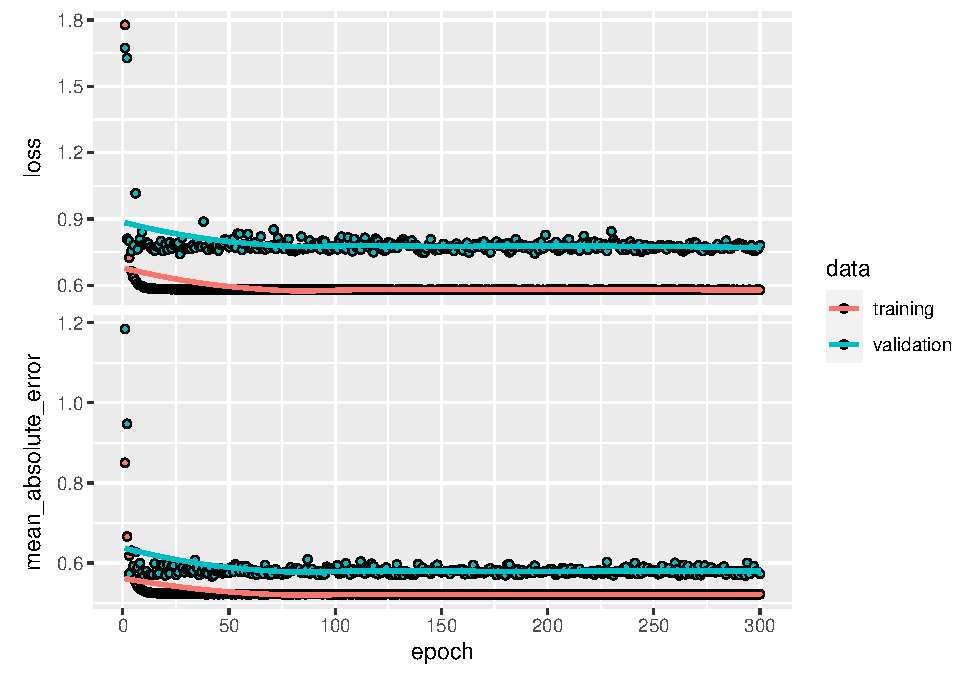
\includegraphics{project_files/figure-latex/unnamed-chunk-52-1.pdf}

\begin{Shaded}
\begin{Highlighting}[]
\KeywordTok{plot}\NormalTok{(history, }\DataTypeTok{metrics =} \StringTok{"mean_absolute_error"}\NormalTok{, }\DataTypeTok{smooth =}\NormalTok{ T) }\OperatorTok{+}
\StringTok{  }\KeywordTok{coord_cartesian}\NormalTok{(}\DataTypeTok{ylim =} \KeywordTok{c}\NormalTok{(}\DecValTok{0}\NormalTok{, }\DecValTok{5}\NormalTok{))}
\end{Highlighting}
\end{Shaded}

\begin{verbatim}
## `geom_smooth()` using formula 'y ~ x'
\end{verbatim}

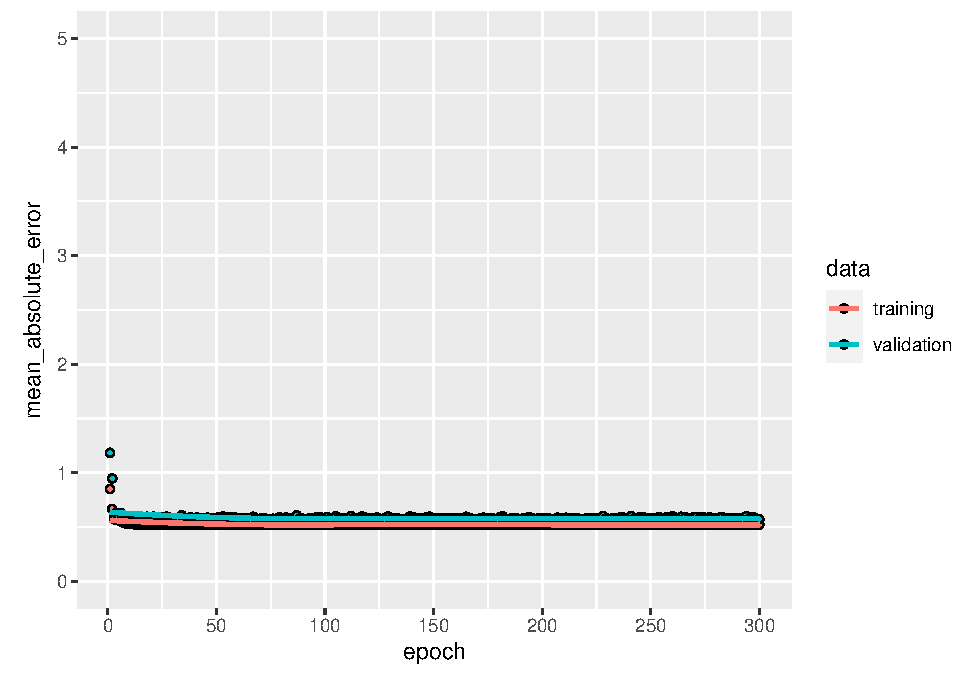
\includegraphics{project_files/figure-latex/unnamed-chunk-52-2.pdf}

\begin{Shaded}
\begin{Highlighting}[]
\NormalTok{eva =}\StringTok{ }\NormalTok{model }\OperatorTok\StringTok{ }\KeywordTok{evaluate}\NormalTok{(feat_test,target_test, }\DataTypeTok{verbose =} \DecValTok{0}\NormalTok{)}

\NormalTok{mae =}\StringTok{ }\NormalTok{eva[}\DecValTok{1}\NormalTok{]}
\NormalTok{loss =}\StringTok{ }\NormalTok{eva[}\DecValTok{2}\NormalTok{]}
\KeywordTok{paste0}\NormalTok{(}\StringTok{"Mean absolute error on test set: "}\NormalTok{, mae)}
\end{Highlighting}
\end{Shaded}

\begin{verbatim}
## [1] "Mean absolute error on test set: 0.60687667131424"
\end{verbatim}

\begin{Shaded}
\begin{Highlighting}[]
\KeywordTok{paste0}\NormalTok{(}\StringTok{"Loss: "}\NormalTok{, loss)}
\end{Highlighting}
\end{Shaded}

\begin{verbatim}
## [1] "Loss: 0.521420836448669"
\end{verbatim}

\begin{Shaded}
\begin{Highlighting}[]
\NormalTok{y_pred =}\StringTok{ }\NormalTok{model }\OperatorTok\StringTok{ }\KeywordTok{predict}\NormalTok{(feat_test)}

\NormalTok{x_axes =}\StringTok{ }\KeywordTok{seq}\NormalTok{(}\DecValTok{1}\OperatorTok{:}\KeywordTok{length}\NormalTok{(y_pred))}
\KeywordTok{plot}\NormalTok{(x_axes, target_test, }\DataTypeTok{type=}\StringTok{"l"}\NormalTok{, }\DataTypeTok{col=}\StringTok{"red"}\NormalTok{)}
\KeywordTok{lines}\NormalTok{(x_axes, y_pred, }\DataTypeTok{col=}\StringTok{"blue"}\NormalTok{)}
\KeywordTok{legend}\NormalTok{(}\StringTok{"topleft"}\NormalTok{, }\DataTypeTok{legend=}\KeywordTok{c}\NormalTok{(}\StringTok{"y-original"}\NormalTok{, }\StringTok{"y-predicted"}\NormalTok{),}
        \DataTypeTok{col=}\KeywordTok{c}\NormalTok{(}\StringTok{"red"}\NormalTok{, }\StringTok{"blue"}\NormalTok{), }\DataTypeTok{lty=}\DecValTok{1}\NormalTok{,}\DataTypeTok{cex=}\FloatTok{0.8}\NormalTok{)}
\end{Highlighting}
\end{Shaded}

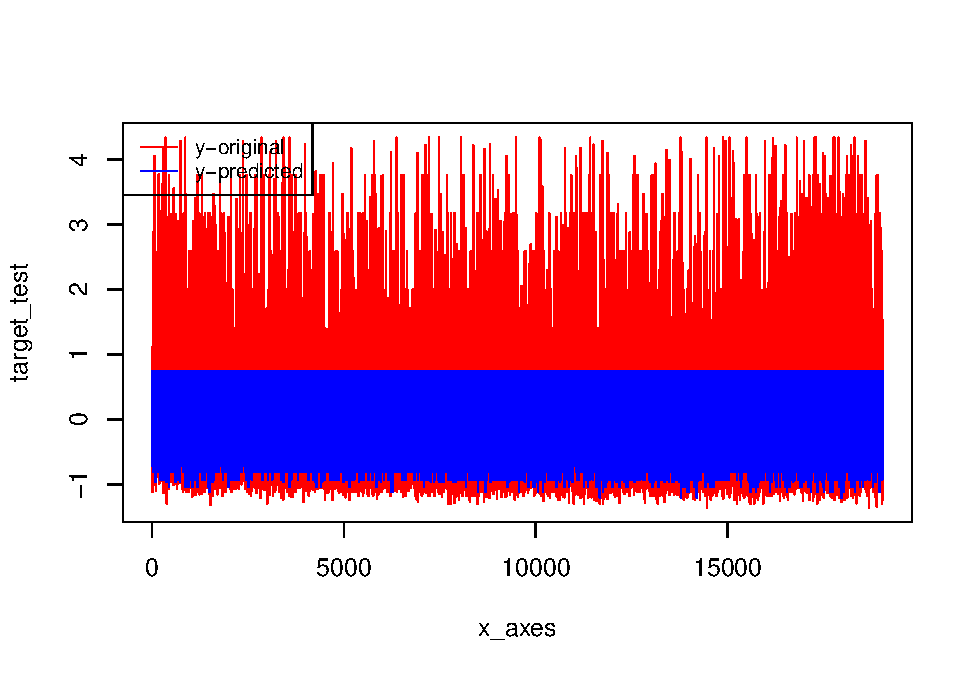
\includegraphics{project_files/figure-latex/unnamed-chunk-54-1.pdf}

\begin{Shaded}
\begin{Highlighting}[]
\NormalTok{MSE.nn =}\StringTok{ }\KeywordTok{mean}\NormalTok{((y_pred}\OperatorTok{-}\NormalTok{target_test)}\OperatorTok{^}\DecValTok{2}\NormalTok{)}
\NormalTok{MSE.nn}
\end{Highlighting}
\end{Shaded}

\begin{verbatim}
## [1] 0.6068767
\end{verbatim}

\begin{Shaded}
\begin{Highlighting}[]
\NormalTok{build_model <-}\StringTok{ }\ControlFlowTok{function}\NormalTok{() \{}
  
\NormalTok{  model <-}\StringTok{ }\KeywordTok{keras_model_sequential}\NormalTok{() }\OperatorTok
\StringTok{    }\KeywordTok{layer_dense}\NormalTok{(}\DataTypeTok{units =} \DecValTok{64}\NormalTok{, }\DataTypeTok{activation =} \StringTok{"relu"}\NormalTok{,}
                \DataTypeTok{input_shape =} \DecValTok{12}\NormalTok{) }\OperatorTok
\StringTok{    }\KeywordTok{layer_dense}\NormalTok{(}\DataTypeTok{units =} \DecValTok{64}\NormalTok{, }\DataTypeTok{activation =} \StringTok{"relu"}\NormalTok{) }\OperatorTok
\StringTok{    }\KeywordTok{layer_dense}\NormalTok{(}\DataTypeTok{units =} \DecValTok{1}\NormalTok{)}
  
\NormalTok{  model }\OperatorTok\StringTok{ }\KeywordTok{compile}\NormalTok{(}
    \DataTypeTok{loss =} \StringTok{"mse"}\NormalTok{,}
    \DataTypeTok{optimizer =} \KeywordTok{optimizer_rmsprop}\NormalTok{(),}
    \DataTypeTok{metrics =} \KeywordTok{list}\NormalTok{(}\StringTok{"mean_absolute_error"}\NormalTok{)}
\NormalTok{  )}
  
\NormalTok{  model}
\NormalTok{\}}

\NormalTok{model <-}\StringTok{ }\KeywordTok{build_model}\NormalTok{()}
\NormalTok{model }\OperatorTok\StringTok{ }\KeywordTok{summary}\NormalTok{()}
\end{Highlighting}
\end{Shaded}

\begin{verbatim}
## Model: "sequential_2"
## ________________________________________________________________________________
## Layer (type)                        Output Shape                    Param #     
## ================================================================================
## dense_6 (Dense)                     (None, 64)                      832         
## ________________________________________________________________________________
## dense_7 (Dense)                     (None, 64)                      4160        
## ________________________________________________________________________________
## dense_8 (Dense)                     (None, 1)                       65          
## ================================================================================
## Total params: 5,057
## Trainable params: 5,057
## Non-trainable params: 0
## ________________________________________________________________________________
\end{verbatim}

\begin{Shaded}
\begin{Highlighting}[]
\CommentTok{# Display training progress by printing a single dot for each completed epoch.}

\NormalTok{print_dot_callback <-}\StringTok{ }\KeywordTok{callback_lambda}\NormalTok{(}
  \DataTypeTok{on_epoch_end =} \ControlFlowTok{function}\NormalTok{(epoch, logs) \{}
    \ControlFlowTok{if}\NormalTok{ (epoch }\OperatorTok\StringTok{ }\DecValTok{80} \OperatorTok{==}\StringTok{ }\DecValTok{0}\NormalTok{) }\KeywordTok{cat}\NormalTok{(}\StringTok{"}\CharTok{\textbackslash{}n}\StringTok{"}\NormalTok{)}
    \KeywordTok{cat}\NormalTok{(}\StringTok{"."}\NormalTok{)}
\NormalTok{  \}}
\NormalTok{)    }

\NormalTok{start.time =}\StringTok{ }\KeywordTok{Sys.time}\NormalTok{()}

\CommentTok{# Fit the model and store training stats}
\NormalTok{history <-}\StringTok{ }\NormalTok{model }\OperatorTok\StringTok{ }\KeywordTok{fit}\NormalTok{(}
\NormalTok{  feat,}
\NormalTok{  target,}
  \DataTypeTok{epochs =}\NormalTok{ epochs,}
  \DataTypeTok{validation_split =} \FloatTok{0.2}\NormalTok{,}
  \DataTypeTok{verbose =} \DecValTok{0}\NormalTok{,}
  \DataTypeTok{callbacks =} \KeywordTok{list}\NormalTok{(print_dot_callback)}
\NormalTok{)}
\end{Highlighting}
\end{Shaded}

\begin{verbatim}
## 
## ................................................................................
## ................................................................................
## ................................................................................
## ............................................................
\end{verbatim}

\begin{Shaded}
\begin{Highlighting}[]
\NormalTok{end.time <-}\StringTok{ }\KeywordTok{Sys.time}\NormalTok{()}
\NormalTok{time.taken <-}\StringTok{ }\NormalTok{end.time }\OperatorTok{-}\StringTok{ }\NormalTok{start.time}

\KeywordTok{print}\NormalTok{(}\StringTok{"-- Time: -- "}\NormalTok{)}
\end{Highlighting}
\end{Shaded}

\begin{verbatim}
## [1] "-- Time: -- "
\end{verbatim}

\begin{Shaded}
\begin{Highlighting}[]
\NormalTok{time.taken}
\end{Highlighting}
\end{Shaded}

\begin{verbatim}
## Time difference of 5.788668 mins
\end{verbatim}

\begin{Shaded}
\begin{Highlighting}[]
\KeywordTok{print}\NormalTok{(}\StringTok{""}\NormalTok{)}
\end{Highlighting}
\end{Shaded}

\begin{verbatim}
## [1] ""
\end{verbatim}

\begin{Shaded}
\begin{Highlighting}[]
\CommentTok{# The patience parameter is the amount of epochs to check for improvement.}
\NormalTok{early_stop <-}\StringTok{ }\KeywordTok{callback_early_stopping}\NormalTok{(}\DataTypeTok{monitor =} \StringTok{"val_loss"}\NormalTok{, }\DataTypeTok{patience =} \DecValTok{20}\NormalTok{)}
\NormalTok{epochs <-}\StringTok{ }\DecValTok{500}

\NormalTok{start.time <-}\StringTok{ }\KeywordTok{Sys.time}\NormalTok{()}

\NormalTok{model <-}\StringTok{ }\KeywordTok{build_model}\NormalTok{()}
\NormalTok{history <-}\StringTok{ }\NormalTok{model }\OperatorTok\StringTok{ }\KeywordTok{fit}\NormalTok{(}
\NormalTok{  feat,}
\NormalTok{  target,}
  \DataTypeTok{epochs =}\NormalTok{ epochs,}
  \DataTypeTok{validation_split =} \FloatTok{0.2}\NormalTok{,}
  \DataTypeTok{verbose =} \DecValTok{0}\NormalTok{,}
  \DataTypeTok{callbacks =} \KeywordTok{list}\NormalTok{(early_stop, print_dot_callback)}
\NormalTok{)}
\end{Highlighting}
\end{Shaded}

\begin{verbatim}
## 
## .........................................
\end{verbatim}

\begin{Shaded}
\begin{Highlighting}[]
\NormalTok{end.time <-}\StringTok{ }\KeywordTok{Sys.time}\NormalTok{()}
\NormalTok{time.taken <-}\StringTok{ }\NormalTok{end.time }\OperatorTok{-}\StringTok{ }\NormalTok{start.time}

\KeywordTok{print}\NormalTok{(}\StringTok{"-- Time: -- "}\NormalTok{)}
\end{Highlighting}
\end{Shaded}

\begin{verbatim}
## [1] "-- Time: -- "
\end{verbatim}

\begin{Shaded}
\begin{Highlighting}[]
\NormalTok{time.taken}
\end{Highlighting}
\end{Shaded}

\begin{verbatim}
## Time difference of 47.9353 secs
\end{verbatim}

\begin{Shaded}
\begin{Highlighting}[]
\KeywordTok{print}\NormalTok{(}\StringTok{""}\NormalTok{)}
\end{Highlighting}
\end{Shaded}

\begin{verbatim}
## [1] ""
\end{verbatim}

\begin{Shaded}
\begin{Highlighting}[]
\NormalTok{history}\OperatorTok{$}\NormalTok{params}\OperatorTok{$}\NormalTok{epochs =}\KeywordTok{length}\NormalTok{(history}\OperatorTok{$}\NormalTok{metrics}\OperatorTok{$}\NormalTok{mean_absolute_error)}

\KeywordTok{plot}\NormalTok{(history, }\DataTypeTok{metrics =} \StringTok{"mean_absolute_error"}\NormalTok{, }\DataTypeTok{smooth =}\NormalTok{ T) }\OperatorTok{+}
\StringTok{  }\KeywordTok{coord_cartesian}\NormalTok{(}\DataTypeTok{xlim =} \KeywordTok{c}\NormalTok{(}\DecValTok{0}\NormalTok{, history}\OperatorTok{$}\NormalTok{params}\OperatorTok{$}\NormalTok{epochs}\OperatorTok{*}\FloatTok{1.2}\NormalTok{), }\DataTypeTok{ylim =} \KeywordTok{c}\NormalTok{(}\DecValTok{0}\NormalTok{, }\FloatTok{1.5}\NormalTok{))}
\end{Highlighting}
\end{Shaded}

\begin{verbatim}
## `geom_smooth()` using formula 'y ~ x'
\end{verbatim}

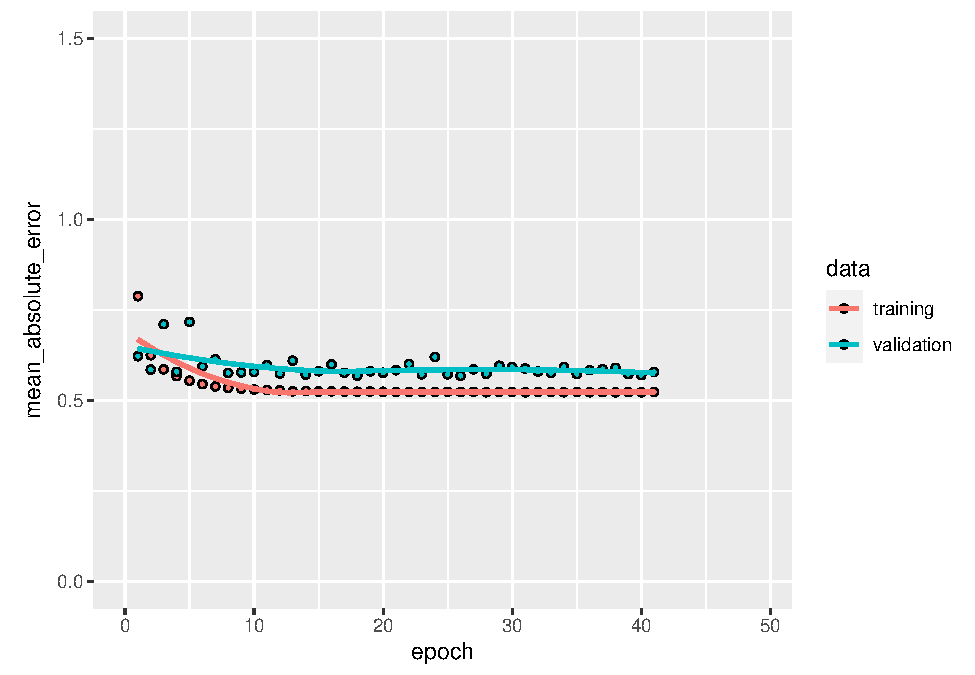
\includegraphics{project_files/figure-latex/unnamed-chunk-57-1.pdf}

\begin{Shaded}
\begin{Highlighting}[]
\NormalTok{eva =}\StringTok{ }\NormalTok{model }\OperatorTok\StringTok{ }\KeywordTok{evaluate}\NormalTok{(feat_test,target_test, }\DataTypeTok{verbose =} \DecValTok{0}\NormalTok{)}

\NormalTok{mae =}\StringTok{ }\NormalTok{eva[}\DecValTok{1}\NormalTok{]}
\NormalTok{loss =}\StringTok{ }\NormalTok{eva[}\DecValTok{2}\NormalTok{]}
\KeywordTok{paste0}\NormalTok{(}\StringTok{"Mean absolute error on test set: "}\NormalTok{, mae)}
\end{Highlighting}
\end{Shaded}

\begin{verbatim}
## [1] "Mean absolute error on test set: 0.613857984542847"
\end{verbatim}

\begin{Shaded}
\begin{Highlighting}[]
\KeywordTok{paste0}\NormalTok{(}\StringTok{"Loss: "}\NormalTok{, loss)}
\end{Highlighting}
\end{Shaded}

\begin{verbatim}
## [1] "Loss: 0.520670652389526"
\end{verbatim}

\begin{Shaded}
\begin{Highlighting}[]
\NormalTok{y_pred =}\StringTok{ }\NormalTok{model }\OperatorTok\StringTok{ }\KeywordTok{predict}\NormalTok{(feat_test)}

\NormalTok{x_axes =}\StringTok{ }\KeywordTok{seq}\NormalTok{(}\DecValTok{1}\OperatorTok{:}\KeywordTok{length}\NormalTok{(y_pred))}
\KeywordTok{plot}\NormalTok{(x_axes, target_test, }\DataTypeTok{type=}\StringTok{"l"}\NormalTok{, }\DataTypeTok{col=}\StringTok{"red"}\NormalTok{)}
\KeywordTok{lines}\NormalTok{(x_axes, y_pred, }\DataTypeTok{col=}\StringTok{"blue"}\NormalTok{)}
\KeywordTok{legend}\NormalTok{(}\StringTok{"topleft"}\NormalTok{, }\DataTypeTok{legend=}\KeywordTok{c}\NormalTok{(}\StringTok{"y-original"}\NormalTok{, }\StringTok{"y-predicted"}\NormalTok{),}
        \DataTypeTok{col=}\KeywordTok{c}\NormalTok{(}\StringTok{"red"}\NormalTok{, }\StringTok{"blue"}\NormalTok{), }\DataTypeTok{lty=}\DecValTok{1}\NormalTok{,}\DataTypeTok{cex=}\FloatTok{0.8}\NormalTok{)}
\end{Highlighting}
\end{Shaded}

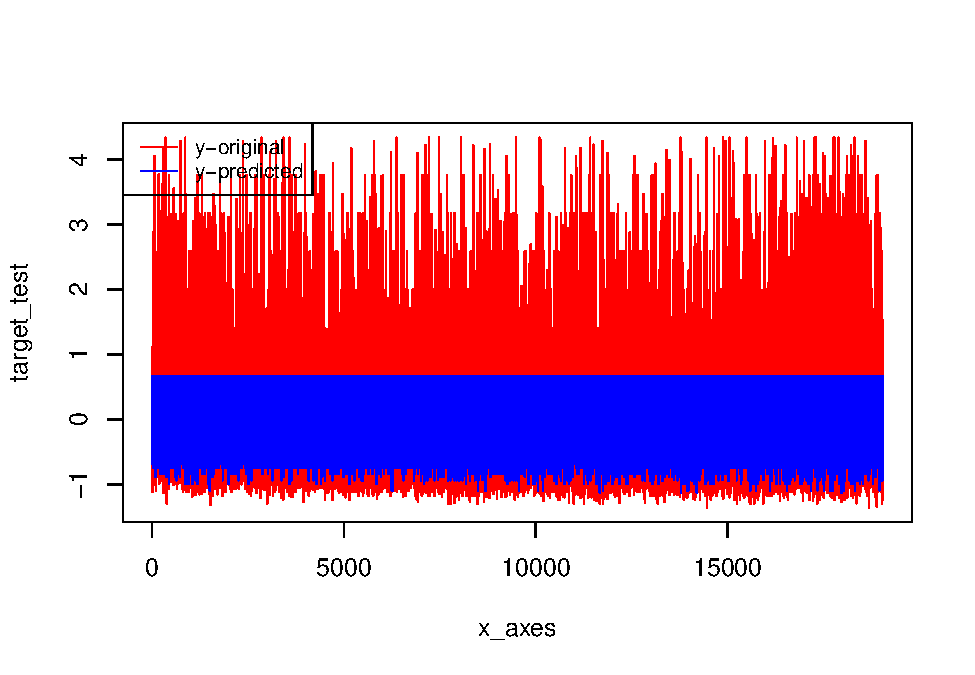
\includegraphics{project_files/figure-latex/unnamed-chunk-59-1.pdf}

\begin{Shaded}
\begin{Highlighting}[]
\NormalTok{MSE.nn =}\StringTok{ }\KeywordTok{mean}\NormalTok{((y_pred}\OperatorTok{-}\NormalTok{target_test)}\OperatorTok{^}\DecValTok{2}\NormalTok{)}
\NormalTok{MSE.nn}
\end{Highlighting}
\end{Shaded}

\begin{verbatim}
## [1] 0.6138579
\end{verbatim}

\begin{Shaded}
\begin{Highlighting}[]
\KeywordTok{library}\NormalTok{(ggplot2)}

\KeywordTok{plot}\NormalTok{(history)}
\end{Highlighting}
\end{Shaded}

\begin{verbatim}
## `geom_smooth()` using formula 'y ~ x'
\end{verbatim}

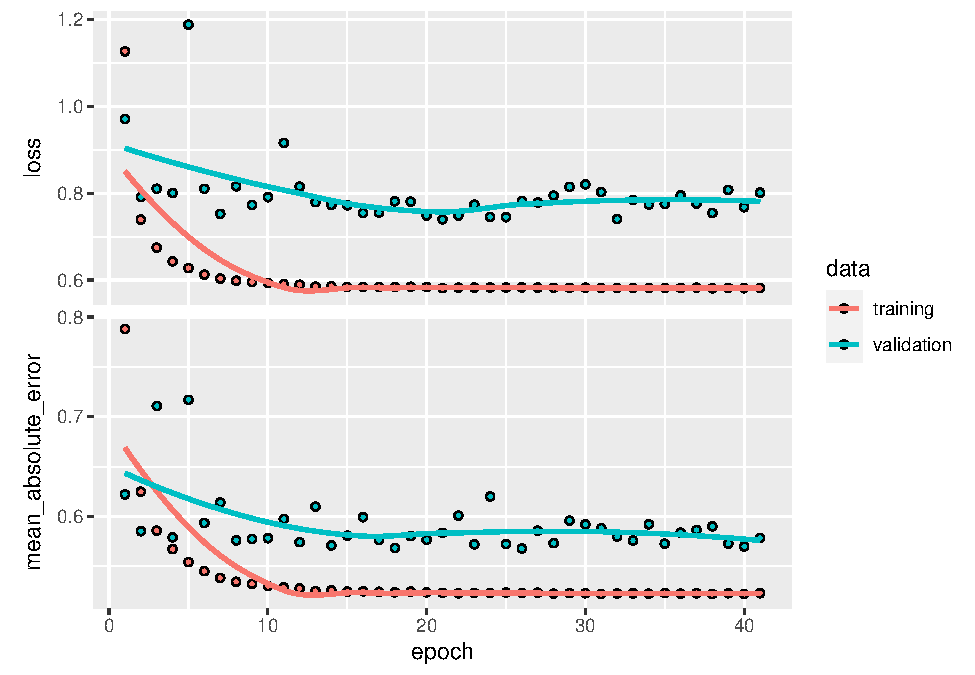
\includegraphics{project_files/figure-latex/unnamed-chunk-60-1.pdf}

\begin{Shaded}
\begin{Highlighting}[]
\KeywordTok{plot}\NormalTok{(history, }\DataTypeTok{metrics =} \StringTok{"mean_absolute_error"}\NormalTok{, }\DataTypeTok{smooth =}\NormalTok{ T) }\OperatorTok{+}
\StringTok{  }\KeywordTok{coord_cartesian}\NormalTok{(}\DataTypeTok{ylim =} \KeywordTok{c}\NormalTok{(}\DecValTok{0}\NormalTok{, }\DecValTok{5}\NormalTok{))}
\end{Highlighting}
\end{Shaded}

\begin{verbatim}
## `geom_smooth()` using formula 'y ~ x'
\end{verbatim}

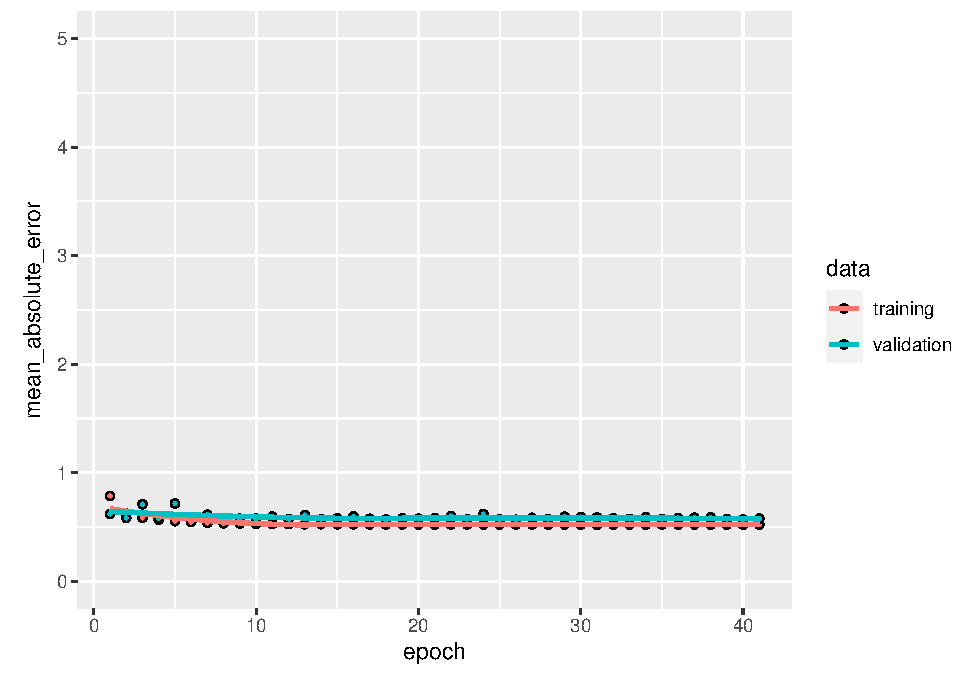
\includegraphics{project_files/figure-latex/unnamed-chunk-60-2.pdf}

\hypertarget{k-means}{%
\section{K-MEANS}\label{k-means}}

\textbf{x}: numeric matrix, numeric data frame or a numeric vector
\textbf{centers}: Possible values are the number of clusters (k) or a
set of initial (distinct) cluster centers. If a number, a random set of
(distinct) rows in x is chosen as the initial centers.
\textbf{iter.max}: The maximum number of iterations allowed. Default
value is 10. \textbf{nstart}: The number of random starting partitions
when centers is a number. Trying nstart \textgreater{} 1 is often
recommended.

\hypertarget{clust-mix-type}{%
\section{Clust miX type}\label{clust-mix-type}}

k-prototypes in RAn implementation of the k-prototypes algorithm is
given by the function

kproto(x, k, lambda = NULL, iter.max = 100, nstart = 1, na.rm = TRUE)

where •x is a data frame with both numeric and factor variables. As
opposed to other existing Rpackages, the factor variables do not need to
be preprocessed in advance and the order of thevariables does not
matter. •k is the number of clusters which has to be pre-specified.
Alternatively, it can also be a vectorof observation indices or a data
frame of prototypes with the same columns asx. If ever atthe
initialization or during the iteration process identical prototypes do
occur, the number ofclusters will be reduced accordingly.

•lambda\textgreater0 is a real valued parameter that controls the trade
off between Euclidean distancefor numeric variables and simple matching
distance for factor variables for cluster assignment.If noλis specified
the parameter is set automatically based on the data and a heuristic
usingthe functionlambdaest(). Alternatively, a vector of
lengthncol(x)can be passed tolambda(cf.Section on Extensions to the
original algorithm).

•iter.maxsets the maximum number of iterations, just as inkmeans(). The
algorithm may stopprior toiter.maxif no observations swap clusters.

•nstartmay be set to a value\textgreater1 to run k-prototypes multiple
times. Similar to k-means, theresult of k-prototypes depends on its
initialization. Ifnstart\textgreater1, the best solution (i.e.~the
onethat minimizesE) is returned.

•Generally, the algorithm can deal with missing data but as a defaultNAs
are removed byna.rm= TRUE

\begin{Shaded}
\begin{Highlighting}[]
\KeywordTok{library}\NormalTok{(clustMixType)}
\KeywordTok{library}\NormalTok{(png)}

\KeywordTok{library}\NormalTok{(ggpubr)}

\NormalTok{clust_num =}\StringTok{ }\DecValTok{5}

\NormalTok{get_clusters =}\StringTok{ }\ControlFlowTok{function}\NormalTok{(dts, num, }\DataTypeTok{factors=}\NormalTok{T)}
\NormalTok{\{}
\NormalTok{  l =}\StringTok{ }\KeywordTok{list}\NormalTok{()}
  \ControlFlowTok{if}\NormalTok{(}\KeywordTok{isFALSE}\NormalTok{(factors))}
\NormalTok{  \{}
\NormalTok{    l}\OperatorTok{$}\NormalTok{cl =}\StringTok{ }\KeywordTok{kmeans}\NormalTok{(dts,num)}
\NormalTok{  \}}
  \ControlFlowTok{else}
\NormalTok{  \{}
\NormalTok{      l}\OperatorTok{$}\NormalTok{cl =}\StringTok{ }\KeywordTok{kproto}\NormalTok{(dts,num)}

\NormalTok{  \}}
  
\NormalTok{  clust =}\StringTok{ }\KeywordTok{list}\NormalTok{()}
  
  \ControlFlowTok{for}\NormalTok{ (i }\ControlFlowTok{in} \DecValTok{1}\OperatorTok{:}\NormalTok{num)}
\NormalTok{  \{}
\NormalTok{    indexes =}\StringTok{ }\NormalTok{l}\OperatorTok{$}\NormalTok{cl}\OperatorTok{$}\NormalTok{cluster }\OperatorTok{==}\StringTok{ }\NormalTok{i}
\NormalTok{    clust[[i]] =}\StringTok{ }\NormalTok{dts[indexes,]}
\NormalTok{  \}}

\NormalTok{  myplot=}\StringTok{ }\KeywordTok{ggplot}\NormalTok{() }\OperatorTok{+}\KeywordTok{background_image}\NormalTok{(img)}\OperatorTok{+}\StringTok{  }\KeywordTok{xlab}\NormalTok{(}\StringTok{'data_date'}\NormalTok{) }\OperatorTok{+}\StringTok{  }\KeywordTok{ylab}\NormalTok{(}\StringTok{'percent.change'}\NormalTok{)}\OperatorTok{+}\StringTok{ }\KeywordTok{theme}\NormalTok{(}\DataTypeTok{plot.margin =} \KeywordTok{unit}\NormalTok{(}\KeywordTok{c}\NormalTok{(}\DecValTok{1}\NormalTok{,}\DecValTok{1}\NormalTok{,}\DecValTok{1}\NormalTok{,}\DecValTok{1}\NormalTok{),}\StringTok{"cm"}\NormalTok{),}\DataTypeTok{legend.title =} \KeywordTok{element_text}\NormalTok{(}\DataTypeTok{colour=}\StringTok{"blue"}\NormalTok{, }\DataTypeTok{size=}\DecValTok{10}\NormalTok{, }\DataTypeTok{face=}\StringTok{"bold"}\NormalTok{))}
\NormalTok{  count =}\StringTok{ }\DecValTok{1}
  \ControlFlowTok{for}\NormalTok{(el }\ControlFlowTok{in}\NormalTok{ clust)}
\NormalTok{  \{}
\NormalTok{    myplot =}\StringTok{ }\NormalTok{myplot}\OperatorTok{+}\KeywordTok{geom_point}\NormalTok{(}\DataTypeTok{data =}\NormalTok{ el, }\KeywordTok{aes}\NormalTok{(}\DataTypeTok{y =}\NormalTok{ latitude, }\DataTypeTok{x =}\NormalTok{ longitude),}\DataTypeTok{color=}\NormalTok{ count) }
    \KeywordTok{plot}\NormalTok{(}\KeywordTok{ggplot}\NormalTok{()}\OperatorTok{+}\KeywordTok{geom_point}\NormalTok{(}\DataTypeTok{data =}\NormalTok{ el, }\KeywordTok{aes}\NormalTok{(}\DataTypeTok{y =}\NormalTok{ latitude, }\DataTypeTok{x =}\NormalTok{ longitude),}\DataTypeTok{color=}\NormalTok{ count) )}
    \KeywordTok{print}\NormalTok{(}\KeywordTok{paste0}\NormalTok{(}\StringTok{"=== clust: "}\NormalTok{,count,}\StringTok{"==="}\NormalTok{))}
    \KeywordTok{print}\NormalTok{(}\KeywordTok{summary}\NormalTok{(el))}
    \KeywordTok{print}\NormalTok{(}\StringTok{"========="}\NormalTok{)}

\NormalTok{    count=}\StringTok{ }\NormalTok{count}\OperatorTok{+}\DecValTok{1}
\NormalTok{  \}}
\NormalTok{  l}\OperatorTok{$}\NormalTok{myplot =}\StringTok{ }\NormalTok{myplot}
  \KeywordTok{return}\NormalTok{(l)}
\NormalTok{\}}
\NormalTok{lis =}\StringTok{ }\KeywordTok{get_clusters}\NormalTok{(dataset, clust_num)}
\end{Highlighting}
\end{Shaded}

\begin{verbatim}
## # NAs in variables:
## neighbourhood_group            latitude           longitude           room_type 
##                   0                   0                   0                   0 
##               price 
##                   0 
## 0 observation(s) with NAs.
## 
## Estimated lambda: 0.5853531
\end{verbatim}

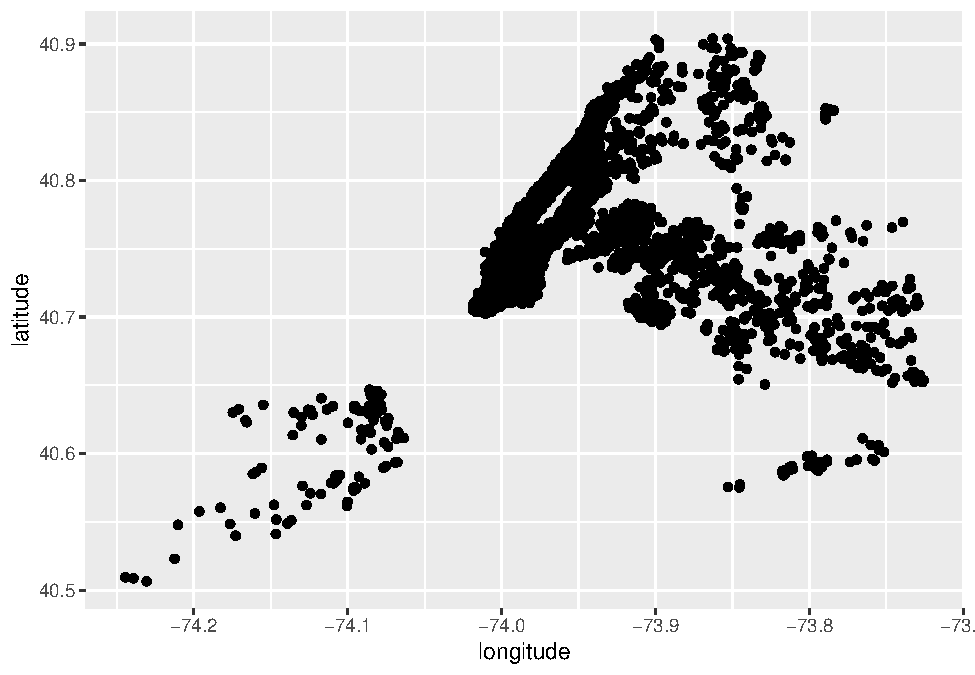
\includegraphics{project_files/figure-latex/unnamed-chunk-61-1.pdf}

\begin{verbatim}
## [1] "=== clust: 1==="
##  neighbourhood_group    latitude       longitude      room_type
##  1:   0              Min.   :40.51   Min.   :-74.24   1:3259   
##  2:8645              1st Qu.:40.73   1st Qu.:-73.99   2:6562   
##  3:1147              Median :40.76   Median :-73.97   3: 339   
##  4: 106              Mean   :40.76   Mean   :-73.96            
##  5: 262              3rd Qu.:40.79   3rd Qu.:-73.95            
##                      Max.   :40.90   Max.   :-73.73            
##      price        
##  Min.   :-1.3538  
##  1st Qu.:-0.3662  
##  Median :-0.1781  
##  Mean   :-0.1704  
##  3rd Qu.: 0.1158  
##  Max.   : 0.4215  
## [1] "========="
\end{verbatim}

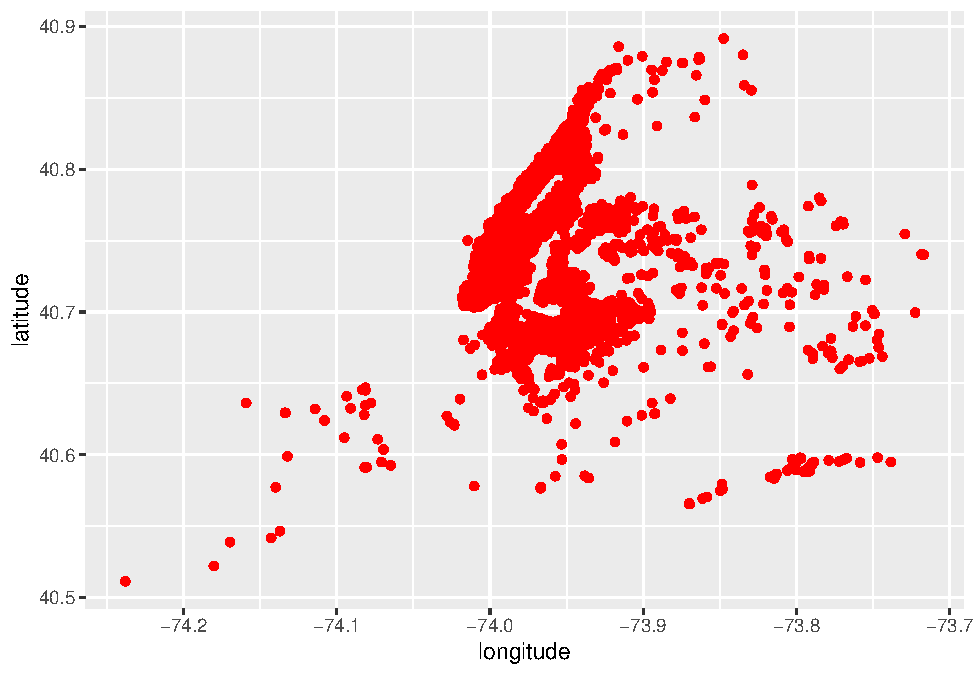
\includegraphics{project_files/figure-latex/unnamed-chunk-61-2.pdf}

\begin{verbatim}
## [1] "=== clust: 2==="
##  neighbourhood_group    latitude       longitude      room_type
##  1:1052              Min.   :40.51   Min.   :-74.24   1: 672   
##  2:5904              1st Qu.:40.72   1st Qu.:-73.99   2:6704   
##  3: 388              Median :40.74   Median :-73.98   3:  24   
##  4:  27              Mean   :40.74   Mean   :-73.97            
##  5:  29              3rd Qu.:40.76   3rd Qu.:-73.96            
##                      Max.   :40.89   Max.   :-73.72            
##      price       
##  Min.   :0.4333  
##  1st Qu.:0.7507  
##  Median :0.9859  
##  Mean   :1.0259  
##  3rd Qu.:1.4092  
##  Max.   :1.8207  
## [1] "========="
\end{verbatim}

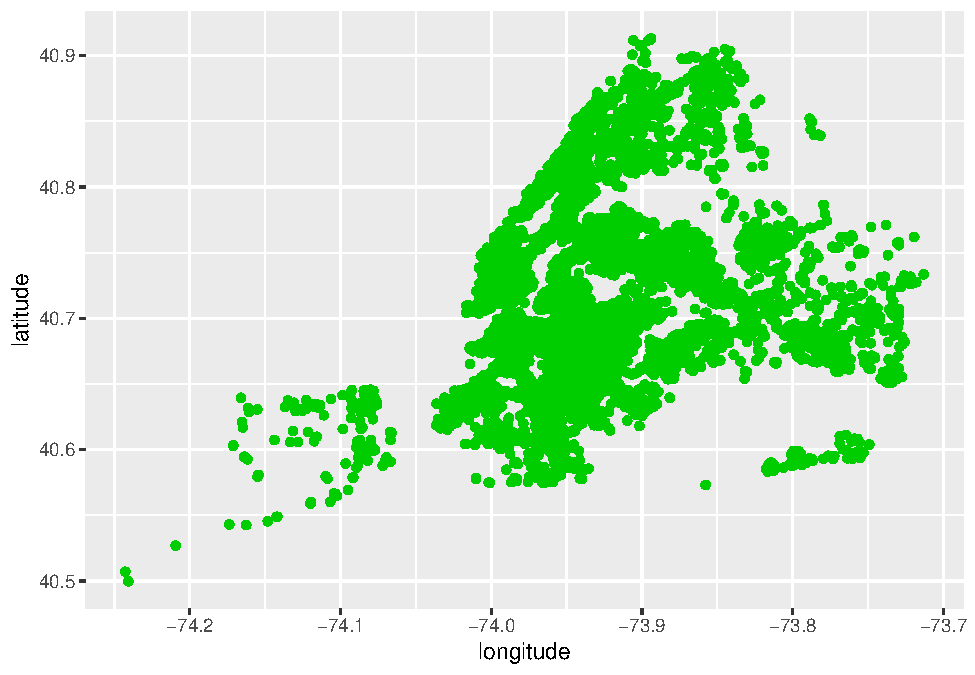
\includegraphics{project_files/figure-latex/unnamed-chunk-61-3.pdf}

\begin{verbatim}
## [1] "=== clust: 3==="
##  neighbourhood_group    latitude       longitude      room_type
##  1:10314             Min.   :40.50   Min.   :-74.24   1:17378  
##  2: 3952             1st Qu.:40.68   1st Qu.:-73.96   2:  456  
##  3: 3415             Median :40.71   Median :-73.94   3:  726  
##  4:  190             Mean   :40.72   Mean   :-73.93            
##  5:  689             3rd Qu.:40.76   3rd Qu.:-73.92            
##                      Max.   :40.91   Max.   :-73.71            
##      price         
##  Min.   :-1.35383  
##  1st Qu.:-0.95407  
##  Median :-0.82474  
##  Mean   :-0.79368  
##  3rd Qu.:-0.64838  
##  Max.   :-0.02524  
## [1] "========="
\end{verbatim}

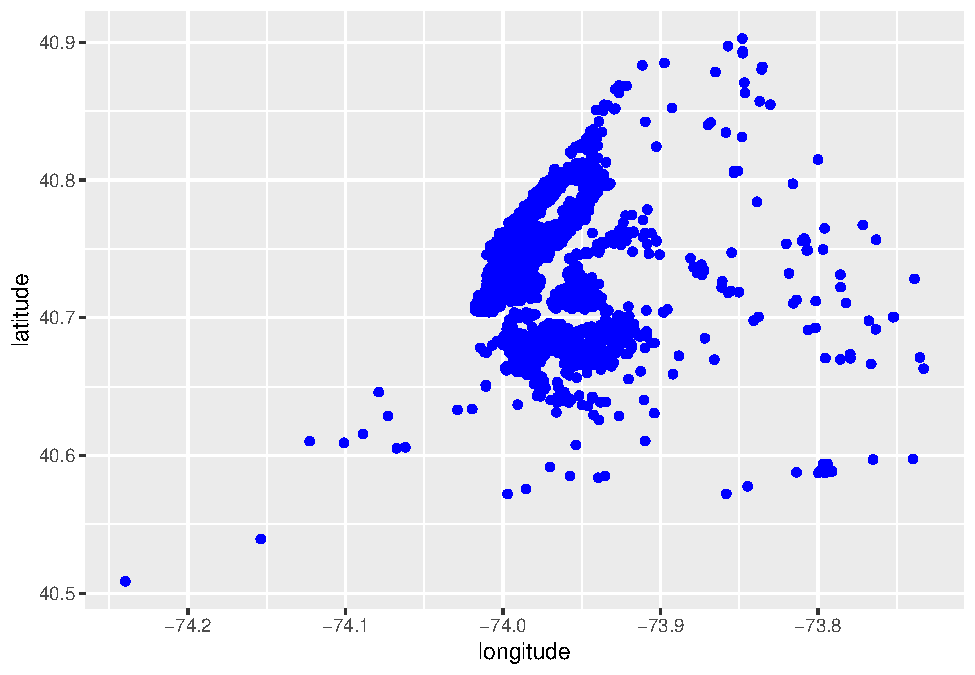
\includegraphics{project_files/figure-latex/unnamed-chunk-61-4.pdf}

\begin{verbatim}
## [1] "=== clust: 4==="
##  neighbourhood_group    latitude       longitude      room_type     price      
##  1: 717              Min.   :40.51   Min.   :-74.24   1: 268    Min.   :1.844  
##  2:2244              1st Qu.:40.72   1st Qu.:-73.99   2:2824    1st Qu.:1.997  
##  3: 116              Median :40.74   Median :-73.98   3:  18    Median :2.585  
##  4:   9              Mean   :40.74   Mean   :-73.97             Mean   :2.652  
##  5:  24              3rd Qu.:40.76   3rd Qu.:-73.96             3rd Qu.:3.161  
##                      Max.   :40.90   Max.   :-73.73             Max.   :4.337  
## [1] "========="
\end{verbatim}

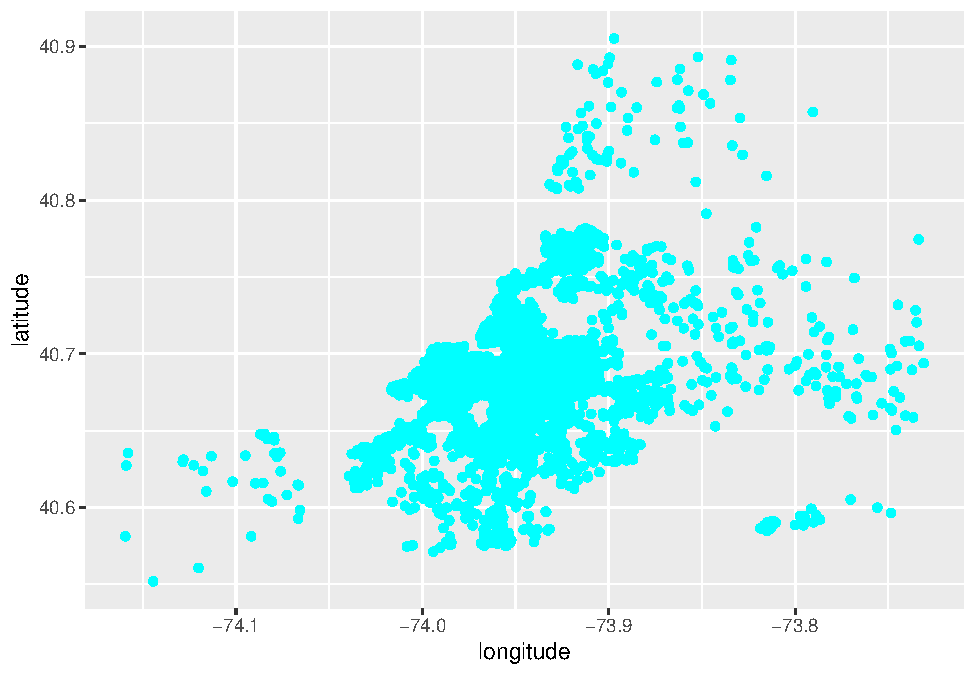
\includegraphics{project_files/figure-latex/unnamed-chunk-61-5.pdf}

\begin{verbatim}
## [1] "=== clust: 5==="
##  neighbourhood_group    latitude       longitude      room_type
##  1:7725              Min.   :40.55   Min.   :-74.16   1: 559   
##  2:   0              1st Qu.:40.67   1st Qu.:-73.97   2:7800   
##  3: 559              Median :40.69   Median :-73.95   3:  35   
##  4:  34              Mean   :40.69   Mean   :-73.95            
##  5:  76              3rd Qu.:40.71   3rd Qu.:-73.94            
##                      Max.   :40.91   Max.   :-73.73            
##      price         
##  Min.   :-0.69541  
##  1st Qu.:-0.26039  
##  Median : 0.05706  
##  Mean   : 0.07423  
##  3rd Qu.: 0.35100  
##  Max.   : 0.85657  
## [1] "========="
\end{verbatim}

\begin{Shaded}
\begin{Highlighting}[]
\NormalTok{lis}\OperatorTok{$}\NormalTok{myplot}
\end{Highlighting}
\end{Shaded}

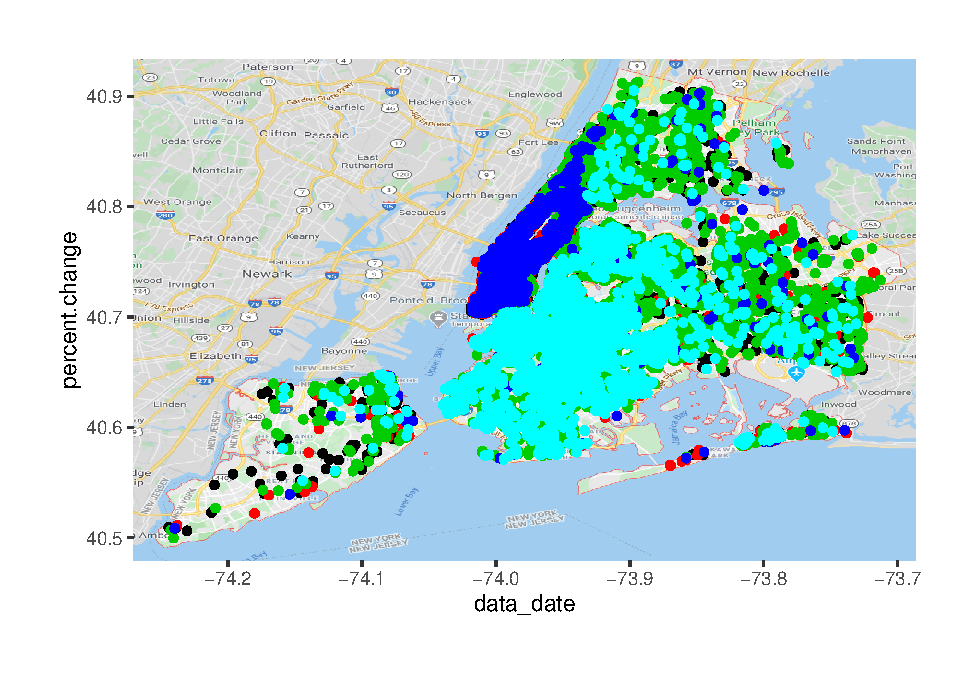
\includegraphics{project_files/figure-latex/unnamed-chunk-61-6.pdf}

\begin{Shaded}
\begin{Highlighting}[]
\NormalTok{lis2 =}\StringTok{ }\KeywordTok{get_clusters}\NormalTok{(ds_neig,}\DecValTok{5}\NormalTok{)}
\end{Highlighting}
\end{Shaded}

\begin{verbatim}
## # NAs in variables:
##  latitude longitude room_type     price 
##         0         0         0         0 
## 0 observation(s) with NAs.
## 
## Estimated lambda: 0.7760002
\end{verbatim}

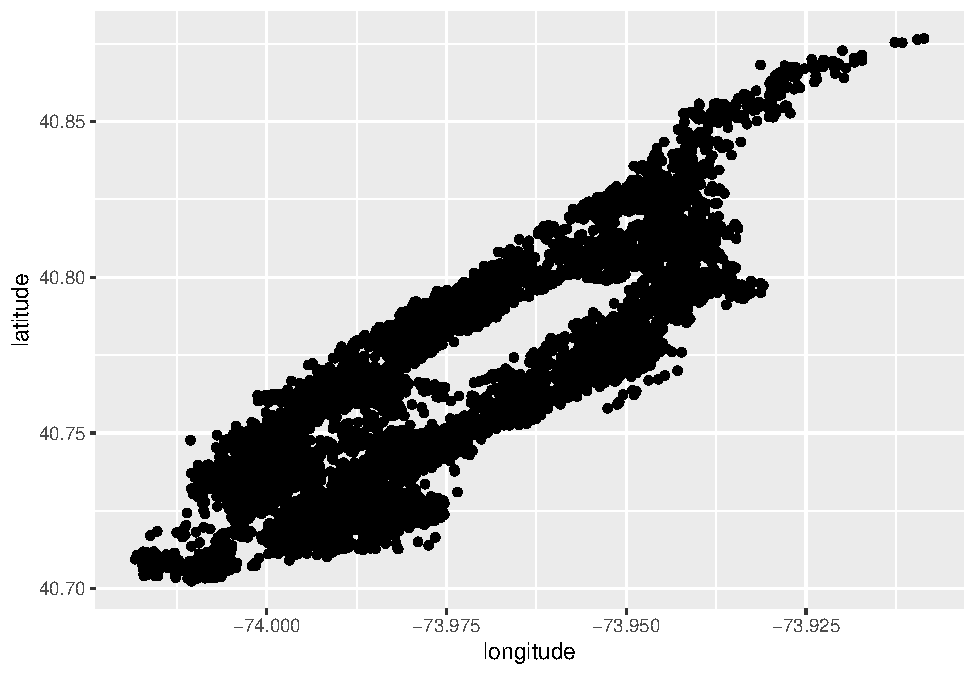
\includegraphics{project_files/figure-latex/unnamed-chunk-61-7.pdf}

\begin{verbatim}
## [1] "=== clust: 1==="
##     latitude       longitude      room_type     price          
##  Min.   :40.70   Min.   :-74.02   1:   0    Min.   :-0.519050  
##  1st Qu.:40.73   1st Qu.:-73.99   2:8648    1st Qu.:-0.001724  
##  Median :40.76   Median :-73.98   3:  13    Median : 0.350998  
##  Mean   :40.76   Mean   :-73.98             Mean   : 0.379158  
##  3rd Qu.:40.78   3rd Qu.:-73.96             3rd Qu.: 0.809536  
##  Max.   :40.88   Max.   :-73.91             Max.   : 1.291590  
## [1] "========="
\end{verbatim}

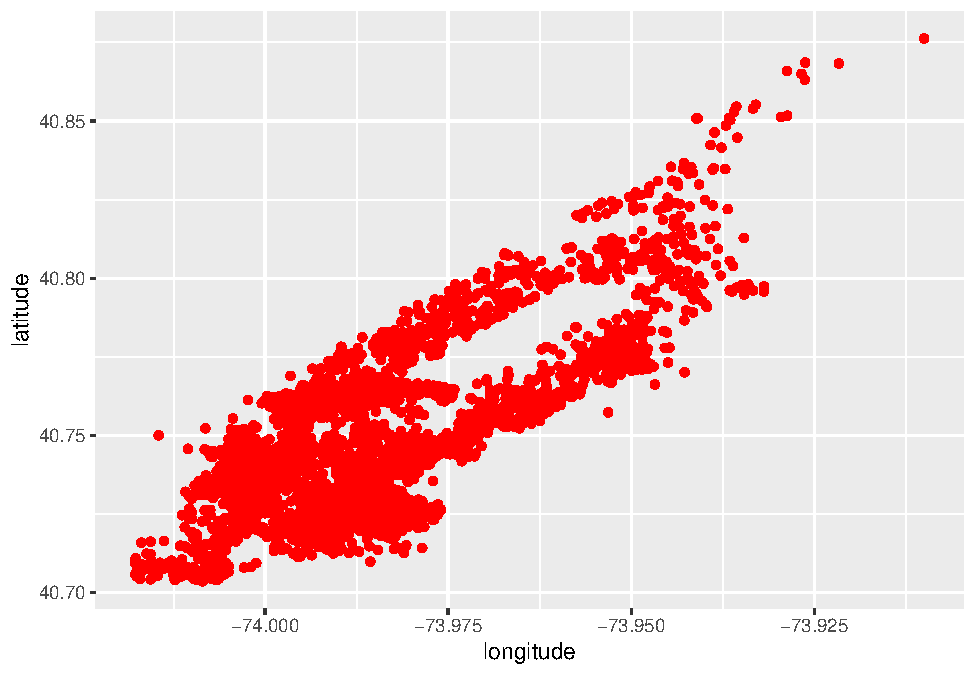
\includegraphics{project_files/figure-latex/unnamed-chunk-61-8.pdf}

\begin{verbatim}
## [1] "=== clust: 2==="
##     latitude       longitude      room_type     price      
##  Min.   :40.70   Min.   :-74.02   1: 229    Min.   :1.303  
##  1st Qu.:40.73   1st Qu.:-74.00   2:3355    1st Qu.:1.527  
##  Median :40.75   Median :-73.99   3:  19    Median :1.997  
##  Mean   :40.75   Mean   :-73.98             Mean   :2.223  
##  3rd Qu.:40.77   3rd Qu.:-73.98             3rd Qu.:2.585  
##  Max.   :40.88   Max.   :-73.91             Max.   :4.337  
## [1] "========="
\end{verbatim}

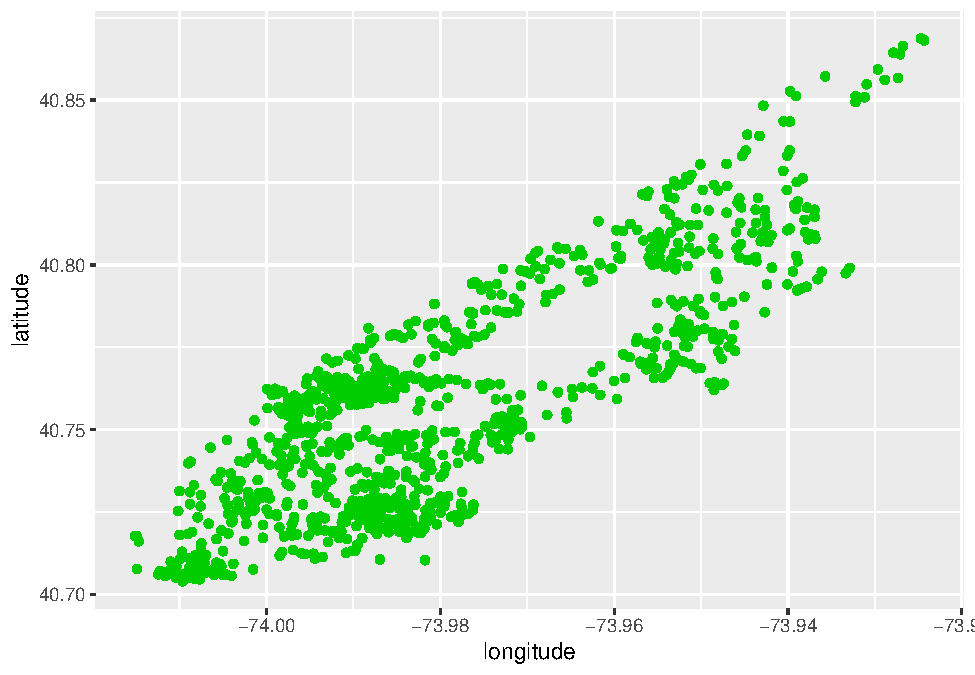
\includegraphics{project_files/figure-latex/unnamed-chunk-61-9.pdf}

\begin{verbatim}
## [1] "=== clust: 3==="
##     latitude       longitude      room_type     price       
##  Min.   :40.70   Min.   :-74.02   1:1069    Min.   :0.1158  
##  1st Qu.:40.73   1st Qu.:-73.99   2:   0    1st Qu.:0.2334  
##  Median :40.76   Median :-73.99   3:  14    Median :0.4568  
##  Mean   :40.76   Mean   :-73.98             Mean   :0.5483  
##  3rd Qu.:40.78   3rd Qu.:-73.97             3rd Qu.:0.8213  
##  Max.   :40.87   Max.   :-73.92             Max.   :1.5738  
## [1] "========="
\end{verbatim}

\includegraphics{project_files/figure-latex/unnamed-chunk-61-10.pdf}

\begin{verbatim}
## [1] "=== clust: 4==="
##     latitude       longitude      room_type     price        
##  Min.   :40.70   Min.   :-74.02   1:3132    Min.   :-0.5543  
##  1st Qu.:40.73   1st Qu.:-73.99   2:  68    1st Qu.:-0.4720  
##  Median :40.76   Median :-73.98   3:  87    Median :-0.3544  
##  Mean   :40.76   Mean   :-73.97             Mean   :-0.3191  
##  3rd Qu.:40.80   3rd Qu.:-73.95             3rd Qu.:-0.1898  
##  Max.   :40.88   Max.   :-73.91             Max.   : 0.1041  
## [1] "========="
\end{verbatim}

\includegraphics{project_files/figure-latex/unnamed-chunk-61-11.pdf}

\begin{verbatim}
## [1] "=== clust: 5==="
##     latitude       longitude      room_type     price        
##  Min.   :40.70   Min.   :-74.02   1:3431    Min.   :-1.3538  
##  1st Qu.:40.76   1st Qu.:-73.98   2: 340    1st Qu.:-0.9306  
##  Median :40.80   Median :-73.95   3: 340    Median :-0.7660  
##  Mean   :40.79   Mean   :-73.96             Mean   :-0.7952  
##  3rd Qu.:40.82   3rd Qu.:-73.94             3rd Qu.:-0.6484  
##  Max.   :40.88   Max.   :-73.91             Max.   :-0.5543  
## [1] "========="
\end{verbatim}

\begin{Shaded}
\begin{Highlighting}[]
\NormalTok{lis2}\OperatorTok{$}\NormalTok{myplot}
\end{Highlighting}
\end{Shaded}

\includegraphics{project_files/figure-latex/unnamed-chunk-61-12.pdf}

\begin{Shaded}
\begin{Highlighting}[]
\NormalTok{lis3 =}\StringTok{ }\KeywordTok{get_clusters}\NormalTok{(ds_neig_room,}\DecValTok{5}\NormalTok{,F)}
\end{Highlighting}
\end{Shaded}

\includegraphics{project_files/figure-latex/unnamed-chunk-61-13.pdf}

\begin{verbatim}
## [1] "=== clust: 1==="
##     latitude       longitude          price        
##  Min.   :40.70   Min.   :-74.02   Min.   :-0.7777  
##  1st Qu.:40.73   1st Qu.:-73.99   1st Qu.:-0.7072  
##  Median :40.79   Median :-73.96   Median :-0.6014  
##  Mean   :40.78   Mean   :-73.97   Mean   :-0.6122  
##  3rd Qu.:40.81   3rd Qu.:-73.95   3rd Qu.:-0.5308  
##  Max.   :40.88   Max.   :-73.91   Max.   :-0.4367  
## [1] "========="
\end{verbatim}

\includegraphics{project_files/figure-latex/unnamed-chunk-61-14.pdf}

\begin{verbatim}
## [1] "=== clust: 2==="
##     latitude       longitude          price        
##  Min.   :40.70   Min.   :-74.02   Min.   :-1.3421  
##  1st Qu.:40.80   1st Qu.:-73.96   1st Qu.:-1.0011  
##  Median :40.82   Median :-73.95   Median :-0.9423  
##  Mean   :40.81   Mean   :-73.95   Mean   :-0.9325  
##  3rd Qu.:40.83   3rd Qu.:-73.94   3rd Qu.:-0.8365  
##  Max.   :40.88   Max.   :-73.91   Max.   :-0.7660  
## [1] "========="
\end{verbatim}

\includegraphics{project_files/figure-latex/unnamed-chunk-61-15.pdf}

\begin{verbatim}
## [1] "=== clust: 3==="
##     latitude       longitude          price         
##  Min.   :40.70   Min.   :-74.02   Min.   :-0.42499  
##  1st Qu.:40.73   1st Qu.:-73.99   1st Qu.:-0.35445  
##  Median :40.76   Median :-73.98   Median :-0.29566  
##  Mean   :40.76   Mean   :-73.98   Mean   :-0.24938  
##  3rd Qu.:40.79   3rd Qu.:-73.96   3rd Qu.:-0.11930  
##  Max.   :40.87   Max.   :-73.92   Max.   : 0.09233  
## [1] "========="
\end{verbatim}

\includegraphics{project_files/figure-latex/unnamed-chunk-61-16.pdf}

\begin{verbatim}
## [1] "=== clust: 4==="
##     latitude       longitude          price       
##  Min.   :40.70   Min.   :-74.02   Min.   :0.1041  
##  1st Qu.:40.73   1st Qu.:-73.99   1st Qu.:0.2334  
##  Median :40.76   Median :-73.99   Median :0.3510  
##  Mean   :40.76   Mean   :-73.98   Mean   :0.4565  
##  3rd Qu.:40.78   3rd Qu.:-73.97   3rd Qu.:0.7037  
##  Max.   :40.87   Max.   :-73.92   Max.   :1.2916  
## [1] "========="
\end{verbatim}

\includegraphics{project_files/figure-latex/unnamed-chunk-61-17.pdf}

\begin{verbatim}
## [1] "=== clust: 5==="
##     latitude       longitude          price      
##  Min.   :40.71   Min.   :-74.01   Min.   :1.339  
##  1st Qu.:40.74   1st Qu.:-73.99   1st Qu.:1.450  
##  Median :40.76   Median :-73.98   Median :1.997  
##  Mean   :40.76   Mean   :-73.98   Mean   :2.219  
##  3rd Qu.:40.76   3rd Qu.:-73.97   3rd Qu.:2.661  
##  Max.   :40.88   Max.   :-73.91   Max.   :4.337  
## [1] "========="
\end{verbatim}

\begin{Shaded}
\begin{Highlighting}[]
\NormalTok{lis3}\OperatorTok{$}\NormalTok{myplot}
\end{Highlighting}
\end{Shaded}

\includegraphics{project_files/figure-latex/unnamed-chunk-61-18.pdf}

library(wesanderson) par(mfrow=c(2,2)) clprofiles(lis\$cl, dataset, col
= wes\_palette(``Royal1'',5, type = ``continuous''))

\begin{Shaded}
\begin{Highlighting}[]
\NormalTok{Es =}\StringTok{ }\KeywordTok{numeric}\NormalTok{(}\DecValTok{10}\NormalTok{)}
\ControlFlowTok{for}\NormalTok{(i }\ControlFlowTok{in} \DecValTok{1}\OperatorTok{:}\DecValTok{10}\NormalTok{)}
\NormalTok{  \{}
\NormalTok{    kpres <-}\StringTok{ }\KeywordTok{kproto}\NormalTok{(dataset, }\DataTypeTok{k =}\NormalTok{ i, }\DataTypeTok{nstart =} \DecValTok{5}\NormalTok{)}
\NormalTok{    Es[i] <-}\StringTok{ }\NormalTok{kpres}\OperatorTok{$}\NormalTok{tot.withinss}
\NormalTok{  \}}
\end{Highlighting}
\end{Shaded}

\begin{verbatim}
## # NAs in variables:
## neighbourhood_group            latitude           longitude           room_type 
##                   0                   0                   0                   0 
##               price 
##                   0 
## 0 observation(s) with NAs.
## 
## Estimated lambda: 0.5853531 
## 
## # NAs in variables:
## neighbourhood_group            latitude           longitude           room_type 
##                   0                   0                   0                   0 
##               price 
##                   0 
## 0 observation(s) with NAs.
## 
## # NAs in variables:
## neighbourhood_group            latitude           longitude           room_type 
##                   0                   0                   0                   0 
##               price 
##                   0 
## 0 observation(s) with NAs.
## 
## # NAs in variables:
## neighbourhood_group            latitude           longitude           room_type 
##                   0                   0                   0                   0 
##               price 
##                   0 
## 0 observation(s) with NAs.
## 
## # NAs in variables:
## neighbourhood_group            latitude           longitude           room_type 
##                   0                   0                   0                   0 
##               price 
##                   0 
## 0 observation(s) with NAs.
## 
## # NAs in variables:
## neighbourhood_group            latitude           longitude           room_type 
##                   0                   0                   0                   0 
##               price 
##                   0 
## 0 observation(s) with NAs.
## 
## Estimated lambda: 0.5853531 
## 
## # NAs in variables:
## neighbourhood_group            latitude           longitude           room_type 
##                   0                   0                   0                   0 
##               price 
##                   0 
## 0 observation(s) with NAs.
## 
## # NAs in variables:
## neighbourhood_group            latitude           longitude           room_type 
##                   0                   0                   0                   0 
##               price 
##                   0 
## 0 observation(s) with NAs.
## 
## # NAs in variables:
## neighbourhood_group            latitude           longitude           room_type 
##                   0                   0                   0                   0 
##               price 
##                   0 
## 0 observation(s) with NAs.
## 
## # NAs in variables:
## neighbourhood_group            latitude           longitude           room_type 
##                   0                   0                   0                   0 
##               price 
##                   0 
## 0 observation(s) with NAs.
## 
## # NAs in variables:
## neighbourhood_group            latitude           longitude           room_type 
##                   0                   0                   0                   0 
##               price 
##                   0 
## 0 observation(s) with NAs.
## 
## Estimated lambda: 0.5853531 
## 
## # NAs in variables:
## neighbourhood_group            latitude           longitude           room_type 
##                   0                   0                   0                   0 
##               price 
##                   0 
## 0 observation(s) with NAs.
## 
## # NAs in variables:
## neighbourhood_group            latitude           longitude           room_type 
##                   0                   0                   0                   0 
##               price 
##                   0 
## 0 observation(s) with NAs.
## 
## # NAs in variables:
## neighbourhood_group            latitude           longitude           room_type 
##                   0                   0                   0                   0 
##               price 
##                   0 
## 0 observation(s) with NAs.
## 
## # NAs in variables:
## neighbourhood_group            latitude           longitude           room_type 
##                   0                   0                   0                   0 
##               price 
##                   0 
## 0 observation(s) with NAs.
## 
## # NAs in variables:
## neighbourhood_group            latitude           longitude           room_type 
##                   0                   0                   0                   0 
##               price 
##                   0 
## 0 observation(s) with NAs.
## 
## Estimated lambda: 0.5853531 
## 
## # NAs in variables:
## neighbourhood_group            latitude           longitude           room_type 
##                   0                   0                   0                   0 
##               price 
##                   0 
## 0 observation(s) with NAs.
## 
## # NAs in variables:
## neighbourhood_group            latitude           longitude           room_type 
##                   0                   0                   0                   0 
##               price 
##                   0 
## 0 observation(s) with NAs.
## 
## # NAs in variables:
## neighbourhood_group            latitude           longitude           room_type 
##                   0                   0                   0                   0 
##               price 
##                   0 
## 0 observation(s) with NAs.
## 
## # NAs in variables:
## neighbourhood_group            latitude           longitude           room_type 
##                   0                   0                   0                   0 
##               price 
##                   0 
## 0 observation(s) with NAs.
## 
## # NAs in variables:
## neighbourhood_group            latitude           longitude           room_type 
##                   0                   0                   0                   0 
##               price 
##                   0 
## 0 observation(s) with NAs.
## 
## Estimated lambda: 0.5853531 
## 
## # NAs in variables:
## neighbourhood_group            latitude           longitude           room_type 
##                   0                   0                   0                   0 
##               price 
##                   0 
## 0 observation(s) with NAs.
## 
## # NAs in variables:
## neighbourhood_group            latitude           longitude           room_type 
##                   0                   0                   0                   0 
##               price 
##                   0 
## 0 observation(s) with NAs.
## 
## # NAs in variables:
## neighbourhood_group            latitude           longitude           room_type 
##                   0                   0                   0                   0 
##               price 
##                   0 
## 0 observation(s) with NAs.
## 
## # NAs in variables:
## neighbourhood_group            latitude           longitude           room_type 
##                   0                   0                   0                   0 
##               price 
##                   0 
## 0 observation(s) with NAs.
## 
## # NAs in variables:
## neighbourhood_group            latitude           longitude           room_type 
##                   0                   0                   0                   0 
##               price 
##                   0 
## 0 observation(s) with NAs.
## 
## Estimated lambda: 0.5853531 
## 
## # NAs in variables:
## neighbourhood_group            latitude           longitude           room_type 
##                   0                   0                   0                   0 
##               price 
##                   0 
## 0 observation(s) with NAs.
## 
## # NAs in variables:
## neighbourhood_group            latitude           longitude           room_type 
##                   0                   0                   0                   0 
##               price 
##                   0 
## 0 observation(s) with NAs.
## 
## # NAs in variables:
## neighbourhood_group            latitude           longitude           room_type 
##                   0                   0                   0                   0 
##               price 
##                   0 
## 0 observation(s) with NAs.
## 
## # NAs in variables:
## neighbourhood_group            latitude           longitude           room_type 
##                   0                   0                   0                   0 
##               price 
##                   0 
## 0 observation(s) with NAs.
## 
## # NAs in variables:
## neighbourhood_group            latitude           longitude           room_type 
##                   0                   0                   0                   0 
##               price 
##                   0 
## 0 observation(s) with NAs.
## 
## Estimated lambda: 0.5853531 
## 
## # NAs in variables:
## neighbourhood_group            latitude           longitude           room_type 
##                   0                   0                   0                   0 
##               price 
##                   0 
## 0 observation(s) with NAs.
## 
## # NAs in variables:
## neighbourhood_group            latitude           longitude           room_type 
##                   0                   0                   0                   0 
##               price 
##                   0 
## 0 observation(s) with NAs.
## 
## # NAs in variables:
## neighbourhood_group            latitude           longitude           room_type 
##                   0                   0                   0                   0 
##               price 
##                   0 
## 0 observation(s) with NAs.
## 
## # NAs in variables:
## neighbourhood_group            latitude           longitude           room_type 
##                   0                   0                   0                   0 
##               price 
##                   0 
## 0 observation(s) with NAs.
## 
## # NAs in variables:
## neighbourhood_group            latitude           longitude           room_type 
##                   0                   0                   0                   0 
##               price 
##                   0 
## 0 observation(s) with NAs.
## 
## Estimated lambda: 0.5853531 
## 
## # NAs in variables:
## neighbourhood_group            latitude           longitude           room_type 
##                   0                   0                   0                   0 
##               price 
##                   0 
## 0 observation(s) with NAs.
## 
## # NAs in variables:
## neighbourhood_group            latitude           longitude           room_type 
##                   0                   0                   0                   0 
##               price 
##                   0 
## 0 observation(s) with NAs.
## 
## # NAs in variables:
## neighbourhood_group            latitude           longitude           room_type 
##                   0                   0                   0                   0 
##               price 
##                   0 
## 0 observation(s) with NAs.
## 
## # NAs in variables:
## neighbourhood_group            latitude           longitude           room_type 
##                   0                   0                   0                   0 
##               price 
##                   0 
## 0 observation(s) with NAs.
## 
## # NAs in variables:
## neighbourhood_group            latitude           longitude           room_type 
##                   0                   0                   0                   0 
##               price 
##                   0 
## 0 observation(s) with NAs.
## 
## Estimated lambda: 0.5853531 
## 
## # NAs in variables:
## neighbourhood_group            latitude           longitude           room_type 
##                   0                   0                   0                   0 
##               price 
##                   0 
## 0 observation(s) with NAs.
## 
## # NAs in variables:
## neighbourhood_group            latitude           longitude           room_type 
##                   0                   0                   0                   0 
##               price 
##                   0 
## 0 observation(s) with NAs.
## 
## # NAs in variables:
## neighbourhood_group            latitude           longitude           room_type 
##                   0                   0                   0                   0 
##               price 
##                   0 
## 0 observation(s) with NAs.
## 
## # NAs in variables:
## neighbourhood_group            latitude           longitude           room_type 
##                   0                   0                   0                   0 
##               price 
##                   0 
## 0 observation(s) with NAs.
## 
## # NAs in variables:
## neighbourhood_group            latitude           longitude           room_type 
##                   0                   0                   0                   0 
##               price 
##                   0 
## 0 observation(s) with NAs.
## 
## Estimated lambda: 0.5853531 
## 
## # NAs in variables:
## neighbourhood_group            latitude           longitude           room_type 
##                   0                   0                   0                   0 
##               price 
##                   0 
## 0 observation(s) with NAs.
## 
## # NAs in variables:
## neighbourhood_group            latitude           longitude           room_type 
##                   0                   0                   0                   0 
##               price 
##                   0 
## 0 observation(s) with NAs.
## 
## # NAs in variables:
## neighbourhood_group            latitude           longitude           room_type 
##                   0                   0                   0                   0 
##               price 
##                   0 
## 0 observation(s) with NAs.
## 
## # NAs in variables:
## neighbourhood_group            latitude           longitude           room_type 
##                   0                   0                   0                   0 
##               price 
##                   0 
## 0 observation(s) with NAs.
\end{verbatim}

\begin{Shaded}
\begin{Highlighting}[]
\KeywordTok{plot}\NormalTok{(}\DecValTok{1}\OperatorTok{:}\DecValTok{10}\NormalTok{, Es, }\DataTypeTok{type =} \StringTok{"b"}\NormalTok{, }\DataTypeTok{ylab =} \StringTok{"Objective Function"}\NormalTok{, }\DataTypeTok{xlab =} \StringTok{"# Clusters"}\NormalTok{,}\DataTypeTok{main =} \StringTok{"Scree Plot"}\NormalTok{) }
\end{Highlighting}
\end{Shaded}

\includegraphics{project_files/figure-latex/unnamed-chunk-62-1.pdf}

d \textless- dist(dataset, method = ``euclidean'') \# distance matrix
fit \textless- hclust(d, method=``complete'') plot(fit) \# display
dendogram groups \textless- cutree(fit, k=5) \# cut tree into 5 clusters
\# draw dendogram with red borders around the 5 clusters
rect.hclust(fit, k=5, border=``red'')

\begin{Shaded}
\begin{Highlighting}[]
\NormalTok{km.res <-}\StringTok{ }\KeywordTok{kmeans}\NormalTok{(ds_neig_room, }\DecValTok{5}\NormalTok{)}

\CommentTok{# Cluster Plot against 1st 2 principal components}

\CommentTok{# vary parameters for most readable graph}
\KeywordTok{library}\NormalTok{(cluster)}
\KeywordTok{clusplot}\NormalTok{(ds_neig_room, km.res}\OperatorTok{$}\NormalTok{cluster, }\DataTypeTok{color=}\OtherTok{TRUE}\NormalTok{, }\DataTypeTok{shade=}\OtherTok{TRUE}\NormalTok{,}
   \DataTypeTok{labels=}\DecValTok{2}\NormalTok{, }\DataTypeTok{lines=}\DecValTok{0}\NormalTok{)}
\end{Highlighting}
\end{Shaded}

\includegraphics{project_files/figure-latex/unnamed-chunk-63-1.pdf}

\begin{Shaded}
\begin{Highlighting}[]
\CommentTok{# Centroid Plot against 1st 2 discriminant functions}
\KeywordTok{library}\NormalTok{(fpc)}
\KeywordTok{plotcluster}\NormalTok{(ds_neig_room, km.res}\OperatorTok{$}\NormalTok{cluster) }
\end{Highlighting}
\end{Shaded}

\includegraphics{project_files/figure-latex/unnamed-chunk-63-2.pdf}

To create a beautiful graph of the clusters generated with the kmeans()
function, will use the factoextra package.

\begin{Shaded}
\begin{Highlighting}[]
\KeywordTok{library}\NormalTok{(factoextra)}
\end{Highlighting}
\end{Shaded}

\begin{verbatim}
## Welcome! Want to learn more? See two factoextra-related books at https://goo.gl/ve3WBa
\end{verbatim}

Cluster number for each of the observations

\begin{Shaded}
\begin{Highlighting}[]
\KeywordTok{head}\NormalTok{(km.res}\OperatorTok{$}\NormalTok{cluster)}
\end{Highlighting}
\end{Shaded}

\begin{verbatim}
## [1] 2 5 5 5 5 2
\end{verbatim}

Cluster size

\begin{Shaded}
\begin{Highlighting}[]
\NormalTok{km.res}\OperatorTok{$}\NormalTok{size}
\end{Highlighting}
\end{Shaded}

\begin{verbatim}
## [1]  319 1001 1682 2264 2595
\end{verbatim}

Cluster means

\begin{Shaded}
\begin{Highlighting}[]
\NormalTok{km.res}\OperatorTok{$}\NormalTok{centers}
\end{Highlighting}
\end{Shaded}

\begin{verbatim}
##   latitude longitude      price
## 1 40.75528 -73.98149  2.2189140
## 2 40.75885 -73.97988  0.4564502
## 3 40.80836 -73.95218 -0.9324887
## 4 40.76045 -73.97685 -0.2493778
## 5 40.77862 -73.96534 -0.6121852
\end{verbatim}

fviz\_cluster(km.res, data = ds\_neig\_room, palette =
c(``\#00AFBB'',``\#2E9FDF'',``\#0000FF'', ``\#E7B800'', ``\#FC4E07''),
ggtheme = theme\_minimal(), main = ``Partitioning Clustering Plot'' )

res \textless- hcut(ds\_neig\_room, k = 5, stand = FALSE)
fviz\_dend(res, rect = TRUE, cex = 0.5, k\_colors =
c(``\#00AFBB'',``\#2E9FDF'', ``\#0000FF'',``\#E7B800'', ``\#FC4E07''))

\hypertarget{partitioning-around-medoids-pam-algorithm}{%
\section{Partitioning Around Medoids (PAM)
ALGORITHM}\label{partitioning-around-medoids-pam-algorithm}}

\url{https://dpmartin42.github.io/posts/r/cluster-mixed-types}

\url{https://towardsdatascience.com/clustering-on-mixed-type-data-8bbd0a2569c3}

\begin{Shaded}
\begin{Highlighting}[]
\KeywordTok{library}\NormalTok{(cluster)}
\KeywordTok{library}\NormalTok{(readr)}
\KeywordTok{library}\NormalTok{(Rtsne)}
\end{Highlighting}
\end{Shaded}

Compute Gower distance

\begin{Shaded}
\begin{Highlighting}[]
\NormalTok{reduced =}\StringTok{ }\NormalTok{ds_neig =}\StringTok{  }\NormalTok{dataset }\OperatorTok\StringTok{ }\KeywordTok{filter}\NormalTok{(neighbourhood_group }\OperatorTok{==}\StringTok{ }\DecValTok{3}\NormalTok{)}

\CommentTok{#reduced <- dataset[ sample(1:nrow(dataset), nrow(dataset)/5) , ]}

\CommentTok{#print(dim(reduced))}
\NormalTok{gower_dist <-}\StringTok{ }\KeywordTok{daisy}\NormalTok{(reduced, }\DataTypeTok{metric =} \StringTok{"gower"}\NormalTok{)}
\CommentTok{#proxy::simil(reduced, method = "gower")}
\CommentTok{#dim(gower_dist)}
\end{Highlighting}
\end{Shaded}

\begin{Shaded}
\begin{Highlighting}[]
\NormalTok{hc1 <-}\StringTok{ }\KeywordTok{hclust}\NormalTok{(gower_dist, }\DataTypeTok{method =} \StringTok{"complete"}\NormalTok{ )}
\NormalTok{hc1}
\end{Highlighting}
\end{Shaded}

\begin{verbatim}
## 
## Call:
## hclust(d = gower_dist, method = "complete")
## 
## Cluster method   : complete 
## Number of objects: 5625
\end{verbatim}

\begin{Shaded}
\begin{Highlighting}[]
\KeywordTok{plot}\NormalTok{(hc1, }\DataTypeTok{cex =} \FloatTok{0.6}\NormalTok{, }\DataTypeTok{hang =} \DecValTok{-1}\NormalTok{)}
\end{Highlighting}
\end{Shaded}

\includegraphics{project_files/figure-latex/unnamed-chunk-70-1.pdf}

start.time \textless- Sys.time() sil\_width \textless- c(NA) for(i in
2:8)\{\\
pam\_fit \textless- pam(gower\_dist, diss = TRUE, k = i)\\
sil\_width{[}i{]} \textless- pam\_fit\(silinfo\)avg.width\\
\}

end.time \textless- Sys.time() time.taken \textless- end.time -
start.time

print(``-- Time: --'') time.taken print("")

plot(1:8, sil\_width, xlab = ``Number of clusters'', ylab = ``Silhouette
Width'') lines(1:8, sil\_width)

\hypertarget{famd}{%
\section{FAMD}\label{famd}}

\url{http://www.sthda.com/english/articles/31-principal-component-methods-in-r-practical-guide/115-famd-factor-analysis-of-mixed-data-in-r-essentials/}
\url{https://nextjournal.com/pc-methods/calculate-pc-mixed-data}
\url{https://cran.r-project.org/web/packages/FactoMineR/index.html}
\url{https://stats.stackexchange.com/questions/5774/can-principal-component-analysis-be-applied-to-datasets-containing-a-mix-of-cont}

\begin{Shaded}
\begin{Highlighting}[]
\KeywordTok{library}\NormalTok{(}\StringTok{"FactoMineR"}\NormalTok{)}
\KeywordTok{library}\NormalTok{(}\StringTok{"factoextra"}\NormalTok{)}
\end{Highlighting}
\end{Shaded}

FAMD (base, ncp = 5, sup.var = NULL, ind.sup = NULL, graph = TRUE) -
base : a data frame with n rows (individuals) and p columns (variables).
- ncp: the number of dimensions kept in the results (by default 5) -
sup.var: a vector indicating the indexes of the supplementary variables.
- ind.sup: a vector indicating the indexes of the supplementary
individuals. - graph : a logical value. If TRUE a graph is displayed.

\begin{Shaded}
\begin{Highlighting}[]
\NormalTok{res.famd <-}\StringTok{ }\KeywordTok{FAMD}\NormalTok{(dataset, }\DataTypeTok{graph =} \OtherTok{FALSE}\NormalTok{, }\DataTypeTok{ncp =} \DecValTok{10}\NormalTok{)}
\KeywordTok{print}\NormalTok{(res.famd)}
\end{Highlighting}
\end{Shaded}

\begin{verbatim}
## *The results are available in the following objects:
## 
##   name          description                             
## 1 "$eig"        "eigenvalues and inertia"               
## 2 "$var"        "Results for the variables"             
## 3 "$ind"        "results for the individuals"           
## 4 "$quali.var"  "Results for the qualitative variables" 
## 5 "$quanti.var" "Results for the quantitative variables"
\end{verbatim}

\begin{Shaded}
\begin{Highlighting}[]
\NormalTok{eig.val <-}\StringTok{ }\KeywordTok{get_eigenvalue}\NormalTok{(res.famd)}
\KeywordTok{head}\NormalTok{(eig.val)}
\end{Highlighting}
\end{Shaded}

\begin{verbatim}
##       eigenvalue variance.percent cumulative.variance.percent
## Dim.1   2.137748         23.75276                    23.75276
## Dim.2   1.805218         20.05798                    43.81074
## Dim.3   1.249605         13.88450                    57.69523
## Dim.4   1.002652         11.14058                    68.83581
## Dim.5   0.997371         11.08190                    79.91771
## Dim.6   0.957535         10.63928                    90.55699
\end{verbatim}

\begin{Shaded}
\begin{Highlighting}[]
\KeywordTok{fviz_screeplot}\NormalTok{(res.famd)}
\end{Highlighting}
\end{Shaded}

\includegraphics{project_files/figure-latex/unnamed-chunk-73-1.pdf}

\begin{Shaded}
\begin{Highlighting}[]
\NormalTok{var <-}\StringTok{ }\KeywordTok{get_famd_var}\NormalTok{(res.famd)}
\NormalTok{var}
\end{Highlighting}
\end{Shaded}

\begin{verbatim}
## FAMD results for variables 
##  ===================================================
##   Name       Description                      
## 1 "$coord"   "Coordinates"                    
## 2 "$cos2"    "Cos2, quality of representation"
## 3 "$contrib" "Contributions"
\end{verbatim}

\begin{Shaded}
\begin{Highlighting}[]
\CommentTok{# Coordinates of variables}
\KeywordTok{head}\NormalTok{(var}\OperatorTok{$}\NormalTok{coord)}
\end{Highlighting}
\end{Shaded}

\begin{verbatim}
##                          Dim.1       Dim.2      Dim.3        Dim.4        Dim.5
## latitude            0.03817251 0.799942829 0.04979299 0.0016726106 0.0018443311
## longitude           0.57648482 0.126449540 0.16901466 0.0001286546 0.0001808065
## price               0.52646870 0.005289316 0.23304329 0.0004961812 0.0001797568
## neighbourhood_group 0.63434790 0.872021956 0.43570149 0.5311816705 0.4769063680
## room_type           0.36227432 0.001514403 0.36205230 0.4691726517 0.5182597446
##                           Dim.6        Dim.7        Dim.8        Dim.9
## latitude            0.003343990 0.0097573346 0.0382064302 5.726698e-02
## longitude           0.007696492 0.0002012975 0.0862969271 3.354680e-02
## price               0.017781932 0.2063906433 0.0098674271 4.827595e-04
## neighbourhood_group 0.821292614 0.0140794996 0.1289174174 8.555108e-02
## room_type           0.107419933 0.1782744198 0.0009683695 6.385971e-05
\end{verbatim}

\begin{Shaded}
\begin{Highlighting}[]
\CommentTok{# Cos2: quality of representation on the factore map}
\KeywordTok{head}\NormalTok{(var}\OperatorTok{$}\NormalTok{cos2)}
\end{Highlighting}
\end{Shaded}

\begin{verbatim}
##                          Dim.1        Dim.2       Dim.3        Dim.4
## latitude            0.00145714 6.399085e-01 0.002479342 2.797626e-06
## longitude           0.33233475 1.598949e-02 0.028565956 1.655201e-08
## price               0.27716929 2.797686e-05 0.054309174 2.461957e-07
## neighbourhood_group 0.10059931 1.901056e-01 0.047458948 7.053849e-02
## room_type           0.06562134 1.146708e-06 0.065540935 1.100615e-01
##                            Dim.5        Dim.6        Dim.7        Dim.8
## latitude            3.401557e-06 1.118227e-05 9.520558e-05 1.459731e-03
## longitude           3.269101e-08 5.923598e-05 4.052067e-08 7.447160e-03
## price               3.231249e-08 3.161971e-04 4.259710e-02 9.736612e-05
## neighbourhood_group 5.685992e-02 1.686304e-01 4.955808e-05 4.154925e-03
## room_type           1.342966e-01 5.769521e-03 1.589088e-02 4.688698e-07
##                            Dim.9
## latitude            3.279507e-03
## longitude           1.125388e-03
## price               2.330567e-07
## neighbourhood_group 1.829747e-03
## room_type           2.039031e-09
\end{verbatim}

\begin{Shaded}
\begin{Highlighting}[]
\CommentTok{# Contributions to the  dimensions}
\KeywordTok{head}\NormalTok{(var}\OperatorTok{$}\NormalTok{contrib)}
\end{Highlighting}
\end{Shaded}

\begin{verbatim}
##                         Dim.1      Dim.2     Dim.3       Dim.4       Dim.5
## latitude             1.785641 44.3128093  3.984699  0.16681869  0.18491926
## longitude           26.966918  7.0046685 13.525450  0.01283144  0.01812831
## price               24.627254  0.2930015 18.649360  0.04948689  0.01802306
## neighbourhood_group 29.673648 48.3056304 34.867145 52.97768250 47.81634564
## room_type           16.946538  0.0838903 28.973346 46.79318048 51.96258373
##                          Dim.6       Dim.7      Dim.8       Dim.9
## latitude             0.3492291  2.38738888 14.4580814 32.37041334
## longitude            0.8037818  0.04925273 32.6564924 18.96247665
## price                1.8570530 50.49890627  3.7340328  0.27288195
## neighbourhood_group 85.7715538  3.44492037 48.7849429 48.35813107
## room_type           11.2183823 43.61953175  0.3664505  0.03609699
\end{verbatim}

\begin{Shaded}
\begin{Highlighting}[]
\CommentTok{# Plot of variables}
\KeywordTok{fviz_famd_var}\NormalTok{(res.famd, }\DataTypeTok{repel =} \OtherTok{TRUE}\NormalTok{)}
\end{Highlighting}
\end{Shaded}

\includegraphics{project_files/figure-latex/unnamed-chunk-76-1.pdf}

\begin{Shaded}
\begin{Highlighting}[]
\CommentTok{# Contribution to the first dimension}
\KeywordTok{fviz_contrib}\NormalTok{(res.famd, }\StringTok{"var"}\NormalTok{, }\DataTypeTok{axes =} \DecValTok{1}\NormalTok{)}
\end{Highlighting}
\end{Shaded}

\includegraphics{project_files/figure-latex/unnamed-chunk-76-2.pdf}

\begin{Shaded}
\begin{Highlighting}[]
\CommentTok{# Contribution to the second dimension}
\KeywordTok{fviz_contrib}\NormalTok{(res.famd, }\StringTok{"var"}\NormalTok{, }\DataTypeTok{axes =} \DecValTok{2}\NormalTok{)}
\end{Highlighting}
\end{Shaded}

\includegraphics{project_files/figure-latex/unnamed-chunk-76-3.pdf}

\begin{Shaded}
\begin{Highlighting}[]
\CommentTok{# Contribution to the third dimension}
\KeywordTok{fviz_contrib}\NormalTok{(res.famd, }\StringTok{"var"}\NormalTok{, }\DataTypeTok{axes =} \DecValTok{3}\NormalTok{)}
\end{Highlighting}
\end{Shaded}

\includegraphics{project_files/figure-latex/unnamed-chunk-76-4.pdf}

\begin{Shaded}
\begin{Highlighting}[]
\CommentTok{# Contribution to the forth dimension}
\KeywordTok{fviz_contrib}\NormalTok{(res.famd, }\StringTok{"var"}\NormalTok{, }\DataTypeTok{axes =} \DecValTok{4}\NormalTok{)}
\end{Highlighting}
\end{Shaded}

\includegraphics{project_files/figure-latex/unnamed-chunk-76-5.pdf}

\begin{Shaded}
\begin{Highlighting}[]
\CommentTok{# Contribution to the fifth dimension}
\KeywordTok{fviz_contrib}\NormalTok{(res.famd, }\StringTok{"var"}\NormalTok{, }\DataTypeTok{axes =} \DecValTok{5}\NormalTok{)}
\end{Highlighting}
\end{Shaded}

\includegraphics{project_files/figure-latex/unnamed-chunk-76-6.pdf}

\begin{Shaded}
\begin{Highlighting}[]
\CommentTok{# Contribution to the sixth dimension}
\KeywordTok{fviz_contrib}\NormalTok{(res.famd, }\StringTok{"var"}\NormalTok{, }\DataTypeTok{axes =} \DecValTok{6}\NormalTok{)}
\end{Highlighting}
\end{Shaded}

\includegraphics{project_files/figure-latex/unnamed-chunk-76-7.pdf}

\begin{Shaded}
\begin{Highlighting}[]
\CommentTok{# Contribution to the seventh dimension}
\KeywordTok{fviz_contrib}\NormalTok{(res.famd, }\StringTok{"var"}\NormalTok{, }\DataTypeTok{axes =} \DecValTok{7}\NormalTok{)}
\end{Highlighting}
\end{Shaded}

\includegraphics{project_files/figure-latex/unnamed-chunk-76-8.pdf}

\begin{Shaded}
\begin{Highlighting}[]
\CommentTok{# Contribution to the eighth dimension}
\KeywordTok{fviz_contrib}\NormalTok{(res.famd, }\StringTok{"var"}\NormalTok{, }\DataTypeTok{axes =} \DecValTok{8}\NormalTok{)}
\end{Highlighting}
\end{Shaded}

\includegraphics{project_files/figure-latex/unnamed-chunk-76-9.pdf}

\hypertarget{pcamixdata}{%
\section{PCAmixdata}\label{pcamixdata}}

\begin{Shaded}
\begin{Highlighting}[]
\CommentTok{## Import library}
\KeywordTok{library}\NormalTok{(PCAmixdata)}
\end{Highlighting}
\end{Shaded}

\begin{Shaded}
\begin{Highlighting}[]
\CommentTok{## Split mixed dataset into quantitative and qualitative variables}
\CommentTok{## For now excluding the target variable "Churn", which will be added later as a supplementary variable}
\CommentTok{#split <- splitmix(dataset[1:5])  }
\NormalTok{split =}\StringTok{ }\KeywordTok{splitmix}\NormalTok{(dataset)}
\CommentTok{## PCA}
\NormalTok{res.pcamix <-}\StringTok{ }\KeywordTok{PCAmix}\NormalTok{(}\DataTypeTok{X.quanti=}\NormalTok{split}\OperatorTok{$}\NormalTok{X.quanti,  }
                     \DataTypeTok{X.quali=}\NormalTok{split}\OperatorTok{$}\NormalTok{X.quali, }
                     \DataTypeTok{rename.level=}\OtherTok{TRUE}\NormalTok{, }
                     \DataTypeTok{graph=}\OtherTok{FALSE}\NormalTok{, }
                     \DataTypeTok{ndim=}\DecValTok{25}\NormalTok{)}

\NormalTok{res.pcamix}
\end{Highlighting}
\end{Shaded}

\begin{verbatim}
## 
## Call:
## PCAmix(X.quanti = split$X.quanti, X.quali = split$X.quali, ndim = 25,     rename.level = TRUE, graph = FALSE)
## 
## Method = Principal Component of mixed data (PCAmix)
## 
## 
## "name" "description"
## "$eig" "eigenvalues of the principal components (PC) "
## "$ind" "results for the individuals (coord,contrib,cos2)"
## "$quanti" "results for the quantitative variables (coord,contrib,cos2)"
## "$levels" "results for the levels of the qualitative variables (coord,contrib,cos2)"
## "$quali" "results for the qualitative variables (contrib,relative contrib)"
## "$sqload" "squared loadings"
## "$coef" "coef of the linear combinations defining the PC"
\end{verbatim}

\begin{Shaded}
\begin{Highlighting}[]
\CommentTok{## Inspect principal components}
\NormalTok{res.pcamix}\OperatorTok{$}\NormalTok{eig}
\end{Highlighting}
\end{Shaded}

\begin{verbatim}
##       Eigenvalue Proportion Cumulative
## dim 1  2.1377482  23.752758   23.75276
## dim 2  1.8052180  20.057978   43.81074
## dim 3  1.2496047  13.884497   57.69523
## dim 4  1.0026518  11.140575   68.83581
## dim 5  0.9973710  11.081900   79.91771
## dim 6  0.9575350  10.639277   90.55699
## dim 7  0.4087032   4.541147   95.09813
## dim 8  0.2642566   2.936184   98.03432
## dim 9  0.1769115   1.965683  100.00000
\end{verbatim}

\begin{Shaded}
\begin{Highlighting}[]
\CommentTok{# Use Scree Diagram to select the components:}
\KeywordTok{plot}\NormalTok{(res.pcamix}\OperatorTok{$}\NormalTok{eig, }\DataTypeTok{type=}\StringTok{"b"}\NormalTok{, }\DataTypeTok{main=}\StringTok{"Scree Diagram"}\NormalTok{, }\DataTypeTok{xlab=}\StringTok{"Number of Component"}\NormalTok{, }\DataTypeTok{ylab=}\StringTok{"Eigenvalues"}\NormalTok{)}
\KeywordTok{abline}\NormalTok{(}\DataTypeTok{h=}\DecValTok{1}\NormalTok{, }\DataTypeTok{lwd=}\DecValTok{3}\NormalTok{, }\DataTypeTok{col=}\StringTok{"red"}\NormalTok{)}
\end{Highlighting}
\end{Shaded}

\includegraphics{project_files/figure-latex/unnamed-chunk-80-1.pdf}

\hypertarget{hierarchical-cluster-analysis}{%
\section{Hierarchical Cluster
Analysis}\label{hierarchical-cluster-analysis}}

\begin{Shaded}
\begin{Highlighting}[]
\KeywordTok{library}\NormalTok{(cluster)    }\CommentTok{# clustering algorithms}
\KeywordTok{library}\NormalTok{(dendextend) }\CommentTok{# for comparing two dendrograms}
\end{Highlighting}
\end{Shaded}

\begin{verbatim}
## 
## ---------------------
## Welcome to dendextend version 1.13.4
## Type citation('dendextend') for how to cite the package.
## 
## Type browseVignettes(package = 'dendextend') for the package vignette.
## The github page is: https://github.com/talgalili/dendextend/
## 
## Suggestions and bug-reports can be submitted at: https://github.com/talgalili/dendextend/issues
## Or contact: <tal.galili@gmail.com>
## 
##  To suppress this message use:  suppressPackageStartupMessages(library(dendextend))
## ---------------------
\end{verbatim}

\begin{verbatim}
## 
## Attaching package: 'dendextend'
\end{verbatim}

\begin{verbatim}
## The following object is masked from 'package:ggpubr':
## 
##     rotate
\end{verbatim}

\begin{verbatim}
## The following object is masked from 'package:stats':
## 
##     cutree
\end{verbatim}

\#reduced \textless- dataset{[} sample(1:nrow(dataset), nrow(dataset)/10
) , {]} \#d \textless- dist(dataset, method = ``euclidean'')

\hypertarget{hierarchical-clustering-using-complete-linkage}{%
\section{Hierarchical clustering using Complete
Linkage}\label{hierarchical-clustering-using-complete-linkage}}

hc1 \textless- hclust(gower\_dist, method = ``complete'' )

\hypertarget{plot-the-obtained-dendrogram}{%
\section{Plot the obtained
dendrogram}\label{plot-the-obtained-dendrogram}}

plot(hc1, cex = 0.6, hang = -1) plot(cut(hc1, h=75)\$upper,
main=``Second branch of lower tree with cut at h=75'')

\begin{Shaded}
\begin{Highlighting}[]
\CommentTok{# methods to assess}
\CommentTok{#m <- c( "average", "single", "complete", "ward")}
\CommentTok{#names(m) <- c( "average", "single", "complete", "ward")}

\CommentTok{# function to compute coefficient}
\CommentTok{#ac <- function(x) \{}
\CommentTok{#  agnes(reduced, method = x)$ac}
\CommentTok{#\}}

\CommentTok{#library(purrr)}
\CommentTok{#map_dbl(m, ac)}
\end{Highlighting}
\end{Shaded}

hc3 \textless- agnes(ds\_neig\_room, method = ``ward'') pltree(hc3, cex
= 0.6, hang = -1, main = ``Dendrogram of agnes'')


\end{document}
